\documentclass[11pt]{article}
\usepackage[a4paper,margin=19mm]{geometry}
\usepackage[no-math]{fontspec}
\setmainfont{Latin Modern Roman}[SmallCapsFont=Latin Modern Roman Caps]
\usepackage{amsmath,amssymb,amsthm,mathtools,amscd,verbatim,xcolor,graphicx,hyperref}
\hypersetup{hidelinks}
\numberwithin{equation}{section}
\newtheorem{theorem}{Theorem}[section]
\newtheorem{lemma}[theorem]{Lemma}
\newtheorem{proposition}[theorem]{Proposition}
\newtheorem{corollary}[theorem]{Corollary}
\newtheorem{claim}[theorem]{Claim}
\newtheorem{fact}[theorem]{Fact}
\newtheorem{conjecture}[theorem]{Conjecture}
\theoremstyle{definition}
\newtheorem{definition}[theorem]{Definition}
\newtheorem{example}[theorem]{Example}
\newtheorem{remark}[theorem]{Remark}
\newtheorem{question}[theorem]{Question}
\theoremstyle{plain}
\newcommand{\C}{\mathbb C}
\newcommand{\R}{\mathbb R}
\newcommand{\Q}{\mathbb Q}
\newcommand{\Z}{\mathbb Z}
\newcommand{\N}{\mathbb N}
\newcommand{\eee}{\mathrm e}
\newcommand{\cclass}[1]{\textsf{#1}}
\newcommand{\cproblem}[1]{\textsc{#1}}
\newcommand{\ie}{i.\,e.}
\newcommand{\Ie}{I.\,e.}
\newcommand{\eg}{e.\,g.}
\newcommand{\Eg}{E.\,g.}
\newcommand{\phd}{Ph.\,D.}
\newcommand{\msc}{M.\,S.}
\newcommand{\bsc}{B.\,S.}
\newcommand{\expref}[2]{\hyperref[#2]{#1~\ref{#2}}}
\newcommand{\expeqref}[2]{\hyperref[#2]{#1~\eqref{#2}}}
\newcommand{\exprefsilent}[2]{\hyperref[#2]{#1}}
\newcommand{\epfmtdoi}[1]{\href{https://doi.org/#1}{doi:#1}}
\emergencystretch=3em
\usepackage{etoolbox,bm}
\newcommand{\epfmt}[2]{\begingroup\def\TocNativeBibResult{\PackageError{toc-native-compat}{Unsupported bibliography type/record #1/#2}{Only exact source-observed finite records are allowed.}}\TocNativeBibResult\endgroup}
\usepackage{ifthen}
%% Theory of Computing
%% File: v021a004.tex
%% Publication date: August 31, 2025
%% Authors: Yuval Filmus, Massimo Lauria, Mladen Miksa, Jakob Nordstrom, and Marc Vinyals

%
%
%

%
%

%
%
%
%

%
%
%
%
%
%
%
%
%
%
%
%
%
%
%
%
%
%
%
%
%
%

%



%
%
%
   %

    %
    %
    %
    %

%
%
   %

%
%
%
%
%
\usepackage{graphicx}   %

\makeatletter
\NeedsTeXFormat{LaTeX2e}


\RequirePackage{xspace}
\RequirePackage{subcaption}
\RequirePackage{varioref}
\RequirePackage[inline]{enumitem}

\RequirePackage{standalone}
\RequirePackage{tikz}
\usetikzlibrary{calc,positioning,backgrounds,matrix,graphs}
\usetikzlibrary{arrows.meta,shapes.geometric,shapes.callouts,shapes.misc}

\makeatother

%
%
%

\makeatletter
\NeedsTeXFormat{LaTeX2e}




\theoremstyle{plain}
\newtheorem{observation}[theorem]{Observation}
\newtheorem{openproblem}[theorem]{Open Problem}
%    \newtheorem{claim}[theorem]{Claim}
\newtheorem*{SubstitutionTheorem}{\Refth{thm:substitution} (restated)}

\theoremstyle{definition}
\newtheorem{property}[theorem]{Property}


% Referencing theorem-like structures using the ToC command \expref
%    \expref{Theorem}{thm:Markov}

\newcommand{\refth}[1]{\expref{Theorem}{#1}}
\newcommand{\reflem}[1]{\expref{Lemma}{#1}}
\newcommand{\refpr}[1]{\expref{Proposition}{#1}}
\newcommand{\refcor}[1]{\expref{Corollary}{#1}}
\newcommand{\refdef}[1]{\expref{Definition}{#1}}
\newcommand{\refrem}[1]{\expref{Remark}{#1}}
\newcommand{\refobs}[1]{\expref{Observation}{#1}}
\newcommand{\refconj}[1]{\expref{Conjecture}{#1}}
\newcommand{\refex}[1]{\expref{Example}{#1}}
\newcommand{\refproperty}[1]{\expref{Property}{#1}}


% REFERENCES AT START OF SENTENCE
\newcommand{\Refth}[1]{\expref{Theorem}{#1}}
\newcommand{\Reflem}[1]{\expref{Lemma}{#1}}
\newcommand{\Refpr}[1]{\expref{Proposition}{#1}}
\newcommand{\Refcor}[1]{\expref{Corollary}{#1}}
\newcommand{\Refdef}[1]{\expref{Definition}{#1}}
\newcommand{\Refrem}[1]{\expref{Remark}{#1}}
\newcommand{\Refobs}[1]{\expref{Observation}{#1}}
\newcommand{\Refconj}[1]{\expref{Conjecture}{#1}}
\newcommand{\Refex}[1]{\expref{Example}{#1}}

% REFERENCES WITH PAGE NUMBERS
\newcommand{\refthP}[1]{\expref{Theorem}{#1} on page~\pageref{#1}}
\newcommand{\reflemP}[1]{\expref{Lemma}{#1} on page~\pageref{#1}}
\newcommand{\refprP}[1]{\expref{Proposition}{#1} on page~\pageref{#1}}
\newcommand{\refcorP}[1]{\expref{Corollary}{#1} on page~\pageref{#1}}
\newcommand{\refdefP}[1]{\expref{Definition}{#1} on page~\pageref{#1}}
\newcommand{\refremP}[1]{\expref{Remark}{#1} on page~\pageref{#1}}
\newcommand{\refobsP}[1]{\expref{Observation}{#1} on page~\pageref{#1}}
\newcommand{\refconjP}[1]{\expref{Conjecture}{#1} on page~\pageref{#1}}
\newcommand{\refexP}[1]{\expref{Example}{#1} on page~\pageref{#1}}
\newcommand{\refpropertyP}[1]{\expref{Property}{#1} on page~\pageref{#1}}

% SECTIONS
\newcommand{\refsec}[1]{\expref{Section}{#1}}
\newcommand{\Refsec}[1]{\expref{Section}{#1}}

% APPENDICES
\newcommand{\refapp}[1]{\expref{Appendix}{#1}}
\newcommand{\Refapp}[1]{\expref{Appendix}{#1}}

% FIGURES
\newcommand{\reffig}[1]{\expref{Figure}{#1}}
\newcommand{\reffigP}[1]{\expref{Figure}{#1} on page~\pageref{#1}}
\newcommand{\Reffig}[1]{\expref{Figure}{#1}}
\newcommand{\ReffigP}[1]{\expref{Figure}{#1} on page~\pageref{#1}}




\DeclareMathAlphabet{\mathsfsl}{OT1}{cmss}{m}{sl}

\newcommand{\formatfunctiontoset}[1]{\mathit{#1}}

\newcommand{\formuladots}{\cdots}

\newcommand{\Bigoh}[1]{\mathrm{O} \bigl( #1 \bigr)}
\newcommand{\bigoh}[1]{\mathrm{O} ( #1 )}

\newcommand{\Littleoh}[1]{\mathrm{o} \bigl( #1 \bigr)}
\newcommand{\littleoh}[1]{\mathrm{o} ( #1 )}

\newcommand{\bigtheta}[1]{\Theta ( #1 )}

\newcommand{\Bigomega}[1]{\Omega \bigl( #1 \bigr)}
\newcommand{\bigomega}[1]{\Omega ( #1 )}

\DeclareMathOperator{\polylog}{polylog}

\newcommand{\Ceiling}[1]{\bigl \lceil #1 \bigr \rceil}

\newcommand{\minofexpr}[2][]{\min_{#1} \{ #2 \}}

\newcommand{\fieldstd}{\mathbb{F}}

\DeclareMathOperator{\Expop}{E}
\DeclareMathOperator{\Varianceop}{Var}

\newcommand{\PROB}[2][]{\Pr_{#1} \left[ #2 \right]}

\newcommand{\prob}[2][]{\Pr_{#1} [ #2 ]}

\newcommand{\expectation}[2][]{\Expop_{#1} [ #2 ]}

\newcommand{\Variance}[1]{\Varianceop \bigl( #1 \bigr)}
\newcommand{\variance}[1]{\Varianceop ( #1 )}

\newcommand{\twincommandJN}[6]{#1#2#3\vphantom{#2#5}\mspace{-2.05mu}#4.#5#6}

\newcommand{\condprob}[3][]{\prob[#1]{#2  \mid  #3}}

\newcommand{\funcdescr}[3]{\ensuremath{ #1 : #2 \to #3}}

\newcommand{\domainof}[1]{\ensuremath{\mathrm{dom} ( #1 )}}

\newcommand{\edges}[1]{E( #1 )}

\newcommand{\vertices}[1]{V( #1 )}

\newcommand{\set}[1]{\{ #1 \}}
\newcommand{\Set}[1]{\bigl\{ #1 \bigr\}}

\newcommand{\setdescr}[3][\mid]{\set{ #2 #1 #3 }}
\newcommand{\Setdescr}[3][|]{\ifthenelse{\equal{#1}{;}}{\Set{ #2 \,;\, #3 }}
     {\ifthenelse{\equal{#1}{:}}{\Set{ #2 \,:\, #3 }}
     {\twincommandJN{\bigl\{}{#2\,}{\bigl#1}{\bigr}{\,#3}{\bigr\}}}}}

\newcommand{\setsize}[1]{\lvert#1\rvert}

\newcommand{\intersection}{\cap}

\newcommand{\union}{\cup}
\newcommand{\Union}{\bigcup}

\newcommand{\Lor}{\bigvee}

\newcommand{\olnot}[1]{\overline{#1}}

\newcommand{\clwidth}{k}

\newcommand{\xcnf}[1]{\mbox{\ensuremath{#1}-CNF}\xspace}
\newcommand{\kcnf}{\xcnf{\clwidth}}
\newcommand{\xcnfform}[1]{\mbox{\ensuremath{#1}-CNF} formula\xspace}
\newcommand{\kcnfform}{\xcnfform{\clwidth}}
\newcommand{\xclause}[1]{\mbox{\ensuremath{#1}-clause}\xspace}

\newcommand{\complclassformat}[1]{\textrm{\upshape{\textsf{#1}}}\xspace}
\newcommand{\cocomplclass}[1]{\textrm{\upshape{\textsf{co#1}}}\xspace}

\newcommand{\Pclass}{\complclassformat{P}}
\newcommand{\NP}{\complclassformat{NP}}

\newcommand{\coNP}{\cocomplclass{NP}}

\newcommand{\introduceterm}[1]{{\emph{#1}}}

\newcommand{\eqperiod}{\enspace .}
\newcommand{\eqcomma}{\enspace ,}

\newcommand{\wrt}{with respect to\xspace}

\newcommand{\ieComma}{\ie,\ }
\newcommand{\egComma}{for instance,\ }

\newcommand{\etal}{et al.\@\xspace}



\newcommand{\proofsystemsubindexformat}[1]{\scriptscriptstyle{\mathcal{#1}}}

\newcommand{\resnot}{\proofsystemsubindexformat{R}}

\newcommand{\pcnot}{\proofsystemsubindexformat{PC}}
\newcommand{\pcrnot}{\proofsystemsubindexformat{PCR}}

\newcommand{\proofstd}{\pi}

\newcommand{\derives}{\vdash}
\newcommand{\derivof}[4][\derives]
        {{\ensuremath{{#2} : {#3} \, {#1}\, {#4}}}}
\newcommand{\refof}[2]{\derivof{#1}{#2}{\bot}}

\newcommand{\emptycl}{\bot}

\newcommand{\formf}{\ensuremath{F}}

\newcommand{\varx}{\ensuremath{x}}

 \newcommand{\varw}{\ensuremath{w}}

\newcommand{\lita}{\ensuremath{a}}

\newcommand{\cla}{\ensuremath{A}}

\newcommand{\clc}{\ensuremath{C}}
\newcommand{\cld}{\ensuremath{D}}

\newcommand{\clausesetformat}[1]{\ensuremath{\mathbb{#1}}}
\newcommand{\clsc}{\clausesetformat{C}}

\newcommand{\polynomialsetformat}[1]{\mathbb{#1}}
\newcommand{\pcsp}{\polynomialsetformat{P}}

\newcommand{\setsofvarsorlit}[2]{\mathit{#1}({#2})}
\newcommand{\Setsofvarsorlit}[2]{\mathit{#1}\bigl({#2}\bigr)}

\newcommand{\vars}[1]{\setsofvarsorlit{Vars}{#1}}
\newcommand{\lit}[1]{\setsofvarsorlit{Lit}{#1}}

\newcommand{\Lit}[1]{\Setsofvarsorlit{Lit}{#1}}

\newcommand{\restr}{\rho}

\newcommand{\restrict}[2]{{{#1}\!\!\upharpoonright_{#2}}}

\newcommand{\derivabbrev}[2]{\bigl( #1 \vdash #2 \bigr)}
\newcommand{\derivabbrevsmall}[2]{( #1 \vdash #2 )}

\newcommand{\refutabbrev}[1]{\derivabbrev{#1}{\!\bot}}
\newcommand{\refutabbrevsmall}[1]{\derivabbrevsmall{#1}{\!\bot}}

\newcommand{\genericform}[2]{\mathit{#1}\bigl( #2 \bigr)}
\newcommand{\genericformsmall}[2]{\mathit{#1}( #2 )}

\newcommand{\genericref}[3]{{\mathit{#1}}_{#2}\refutabbrev{#3}}
\newcommand{\genericrefsmall}[3]{{\mathit{#1}}_{#2}\refutabbrevsmall{#3}}

\newcommand{\size}[1]{\genericformsmall{S}{#1}}

\newcommand{\sizeofarg}[1]{\genericformsmall{S}{#1}}

\newcommand{\sizeref}[2][]{\genericrefsmall{S}{#1}{#2}}

\newcommand{\length}[1]{\genericformsmall{L}{#1}}

\newcommand{\lengthref}[2][]{\genericrefsmall{L}{#1}{#2}}

\newcommand{\width}[2][]{\genericformsmall{W_{#1}}{#2}}

\newcommand{\widthref}[2][]{\genericrefsmall{W}{#1}{#2}}

\newcommand{\clspaceref}[2][]{\genericrefsmall{Sp}{#1}{#2}}

\newcommand{\mspaceof}[2][]{\genericformsmall{Sp_{#1}}{#2}}

\newcommand{\mspaceref}[2][]{\genericrefsmall{Sp}{#1}{#2}}

\newcommand{\mdegreeof}[2][]{\genericformsmall{Deg_{#1}}{#2}}

\newcommand{\mdegreeref}[2][]{\genericrefsmall{Deg}{#1}{#2}}

\newcommand{\pcconf}{\clausesetformat{P}}

\newcommand{\formulaformat}[1]{\mathit{#1}}

\newcommand{\extendedversion}[1]{\widetilde{#1}}

\newcommand{\pebdeg}{\ensuremath{d}}

\newcommand{\tseitinnot}[2]{\formulaformat{Ts}({#1,#2})}
\newcommand{\tseitinparity}[2]{\ensuremath{\formulaformat{PARITY}_{#1,#2}}}

\newcommand{\fphpnot}[2]{\formulaformat{FPHP}^{#1}_{#2}}
\newcommand{\efphpnot}[2]{\vphantom{\extendedversion{\formulaformat{FPHP}}}
      {\smash{\extendedversion{\formulaformat{FPHP}}}
        \vphantom{\formulaformat{FPHP}}}^{#1}_{#2}}

 \newcommand{\substform}[2]{{#1}[{#2}]}
\newcommand{\xor}{\oplus}
\newcommand{\fstd}{\formf}
\newcommand{\numset}[1]{[#1]}
\newcommand{\stoptime}{\tau}
\newcommand{\farity}{d}
\newcommand{\ntuple}[1]{\bigl( #1 \bigr)}
\newcommand{\predname}{\formatfunctiontoset{pred}}
\newcommand{\prednode}[2][]{\predname_{#1}(#2)}
\newcommand{\tends}{\longrightarrow}
\newcommand{\probspace}{\mathcal}
\newcommand{\psReg}{\probspace{D}}
\newcommand{\psHam}{\probspace{H}}
\newcommand{\eqdef}{\triangleq}

\newcommand{\fcnot}{\proofsystemsubindexformat{FC}}
\newcommand{\BGmodels}[2]{\models_{(#1,#2)}}
\newcommand{\partialmodels}{\BGmodels{\partitionnot}{\assignmentsetnot}}
\newcommand{\partialmodelsprime}{\BGmodels{\partitionnot'}{\assignmentsetnot'}}
\newcommand{\BGpart}[1]{\partitionnot[#1]}
\newcommand{\definingsetofmonomials}{defining set of monomials\xspace}
\newcommand{\satwitness}[1][]{(F';\partitionnot #1, \assignmentsetnot #1, M #1)}
\DeclareMathOperator{\spanset}{Span}
\newcommand{\Span}[1]{\spanset\left({#1}\right)}

\newcommand{\connectivityexpansionnot}{c}
\newcommand{\cyclelengthnot}{b}
\newcommand{\extraedgesnot}{t}
\newcommand{\oppositeassignment}[1]{\overline{#1}}
\newcommand{\chargedgraph}{charged graph\xspace}
\newcommand{\chargedgraphs}{charged graphs\xspace}
\newcommand{\inducedgraph}[1]{\chargedgraph induced by #1\xspace}
\newcommand{\inducedgraphs}[1]{\chargedgraphs induced by #1\xspace}
\newcommand{\nonsplitting}{non-splitting\xspace}
\newcommand{\nonsplittingassignment}{\nonsplitting assignment\xspace}
\newcommand{\Gnonsplittingnot}{non-splitting\xspace}
\newcommand{\Gnonsplitting}{\Gnonsplittingnot}
\newcommand{\flippedassignments}{flipped assignments\xspace}
\newcommand{\Flippedassignments}{Flipped assignments\xspace}
\newcommand{\flip}[2]{\mathit{Flip}(#1,#2)}
\newcommand{\emptyassignment}{\emptyset}
\newcommand{\edgeboundary}[1]{\partial_e(#1)}
 \newcommand{\flippable}{flippable\xspace}

\newcommand{\kextendiblenot}{r}
\newcommand{\kextendible}{\mbox{$\kextendiblenot$-ex}\-tend\-ible\xspace}
\newcommand{\akextendible}{an \mbox{$\kextendiblenot$-ex}\-tend\-ible\xspace}
\newcommand{\kextendibleNok}{extendible\xspace}
\newcommand{\KextendibleNok}{Extendible\xspace}

\newcommand{\partitionnot}{\mathcal{Q}}
\newcommand{\assignmentsetnot}{\mathcal{H}}
\newcommand{\structuredassignmentsnot}[1][]{(\partitionnot #1,\assignmentsetnot #1)}

\newcommand{\kextendfamily}{\ensuremath{\mathcal{F}}\xspace}

\newcommand{\respectfulness}{respectfulness\xspace}
\newcommand{\Respectfulness}{Respectfulness\xspace}

\newcommand{\restrictionproperty}{restriction property\xspace}

\newcommand{\extensionproperty}{extension property\xspace}

\newcommand{\Restrictionpropname}{Restrictability\xspace}
\newcommand{\extensionpropname}{extendibility\xspace}
\newcommand{\Extensionpropname}{Extendibility\xspace}

\newcommand{\formulakwidth}{k}
\newcommand{\fkwidth}{\formulakwidth}

\newcommand{\adpebblenumber}{\ell}
\newcommand{\adduplicatorfamily}{\mathcal{D}}

\newcommand{\nonauthor}{non-author\-i\-tar\-ian\xspace}
\newcommand{\Nonauthor}{Non-authoritarian\xspace}

\newcommand{\setsofvarsorlitsup}[3]{\mathit{#1}^{#2}({#3})}
\newcommand{\variablecopies}[1]{\setsofvarsorlitsup{Vars}{\pebdeg}{#1}}

\newcommand{\varweightconstrained}{totally weight constrained\xspace}

\newcommand{\varneighborhoodclause}[1]{$#1$-neighborhood clause}

\newcommand{\varneighbors}[1]{N(#1)}
\newcommand{\booleanaxiompartial}{B}
\newcommand{\complementarityiter}[1]{T(#1)}
\newcommand{\negativeaxiomiter}[1]{A(#1)}
\newcommand{\remainingpoly}[1]{R(#1)}

  \newenvironment{ourproof}[1][]{\ifthenelse{\equal{#1}{}}{\begin{proof}}
    {\begin{proof}[Proof~{#1}]}
  }
  {\end{proof}}

\newcommand{\tseitinmodpnot}[2]{\formulaformat{Ts}^{p}({#1,#2})}
\newcommand{\tseitinmodpflow}[2]{\ensuremath{\formulaformat{Mod}^{p}_{#1,#2}}}

\newcommand{\tseitincharge}{\chi}

\newcommand{\theauthorYF}{the first author\xspace}

  \newcommand{\mysubsection}[1]{\subsection{#1}}

  \newcommand{\refsecapp}[1]{Section~\ref{#1}}

\makeatother


\begin{document}
\begin{center}{\Large Stable item 742: Constant-factor equivalence of PC and PCR monomial space for totally weight-constrained formulas}\end{center}
\paragraph{Source and attribution.}
Yuval Filmus, Massimo Lauria, Mladen Mikša, Jakob Nordström, and Marc Vinyals, \emph{Towards an Understanding of Polynomial Calculus: New Separations and Lower Bounds}. Theory of Computing 21 (2025), Article 4, publisher source publication August 31, 2025; DOI 10.4086/toc.2025.v021a004. \href{https://theoryofcomputing.org/articles/v021a004/}{Publisher article}. Original human statement/proof/context: \href{https://creativecommons.org/licenses/by/3.0/}{CC BY3.0}.
\paragraph{Selected problem and source scope.}
Prove only the authors' Theorem 8.4 for totally weight-constrained CNF formulas with a constant number of negative literals per clause. The complete neighborhood-monomial replacement and staged Boolean, complementarity and negative-clause axiom derivations, including all intermediate space bounds, are retained. This is a distinct simulation obligation from the substitution lower bound. No unrestricted PC/PCR equivalence is selected; other results are unselected conservative context and supporting claims are uncounted.
\paragraph{Literal source scope and wording.}
The separate modified-framework Appendix A retains the unresolved axiom-download old/new-space inference at native 3818–3824 as literal contextual material. It is neither repaired nor a selected premise of this independent totally-weight-constrained simulation. Other lower-bound branches with documented source questions remain unselected.
\paragraph{Difficulty (editorial): H2.}
The theorem requires a uniform monomial-space simulation despite a negative literal ordinarily expanding into exponentially many PC monomials. The author replaces each formal complement by a neighborhood monomial and supplies staged derivations for Boolean, complementarity, and negative clause axioms while bounding the live intermediate configurations. This source-local simulation is a distinct substantive obligation from the substitution lower bound; the constant-negative-literal hypothesis is essential and retained.
\paragraph{Editorial source boundary.}
Author mathematical TeX and ordering are unchanged. Only journal front matter is replaced by this wrapper; exact authored macros are flattened and separately preserved, and finite source-observed display aliases are defined in the standalone preamble. Original source figure PDFs remain byte-identical, with the documented extensionless logical aliases and their compiler-resolved PDF names representing one figure each; only necessary relative paths change. No generated proof, mathematical repair or independent mathematical refereeing is supplied. 
\clearpage

%
%
%

%
\section{Introduction}
\label{sec:introduction}

Proof complexity studies how hard it is to provide succinct
certificates of unsatisfiability for formulas in propositional logic---\ieComma
proofs that formulas always evaluate to false under any truth value
assignment, where these proofs are verifiable in time polynomial in
their size.
%
It is widely believed that there is no proof system where such
efficiently verifiable proofs can always be  of size at most
polynomial in the size of the formula.
%
Showing this would establish $\NP \neq \coNP$, and hence
$\Pclass \neq \NP$, and the study of proof complexity was initiated by
Cook and Reckhow~\cite{CR79Relative} as an approach towards this
(still very distant) goal.

A second prominent motivation for proof complexity is the connection
to applied SAT solving. 
%
Any algorithm for solving SAT defines a proof system in the
sense that the execution trace of the algorithm constitutes a
polynomial-time verifiable witness of unsatisfiability. %
(Such a witness
is often referred to as a \introduceterm{refutation} rather than a
\introduceterm{proof}, and we will use the two terms interchangeably in
this paper.) %
In the other direction, most modern SAT solvers can in
fact be seen to search for proofs in systems studied in proof
complexity, and upper and lower bounds for these proof systems hence
give information about the potential and limitations of 
such SAT solvers.

In addition to running time, a major concern in SAT solving is memory
consumption. 
In proof complexity, these two resources are modelled by
\introduceterm{proof size/length}
and
\introduceterm{proof space}.
%
It is thus interesting to understand these
complexity measures and how they are related to each other, and such a
study reveals intriguing connections that are also of intrinsic
interest to proof complexity. In this context, it is natural to focus
on proof systems at comparatively low levels in the proof complexity
hierarchy that are, or could plausibly be, used as a basis for SAT
solvers. Such proof systems include resolution and polynomial
calculus. This paper takes as its starting point the former system but
focuses on the latter.

\mysubsection{Previous work}

The \introduceterm{resolution} proof system was introduced
in~\cite{Blake37Thesis}, and is at the foundation
of state-of-the-art SAT solvers based on so-called conflict-driven
clause learning~(CDCL)~%
\cite{BS97UsingCSP,MS99Grasp,MMZZM01Engineering}.
%
In resolution, one derives new disjunctive clauses 
from the clauses of the original CNF formula until 
contradiction is reached.
One of the early breakthroughs in proof complexity was the
%
%
%
moderately exponential %
%
%
%
%
%
%
$\exp(\bigomega{n^{1/3}})$   %
lower bound on proof length 
(measured as the number of clauses in a proof)
obtained by Haken~\cite{Haken85Intractability}.
%
Simply   %
exponential lower bounds---\ieComma
bounds $\exp(\bigomega{n})$
in the size~$n$ of the formula---were 
later  established in~%
\cite{CS88ManyHard,Urquhart87HardExamples}
and other papers.


Ben-Sasson and Wigderson~\cite{BW01ShortProofs}
identified \introduceterm{width}
as a crucial resource, where the width is the
size of a largest clause in a resolution proof.
They proved that strong lower bounds on width imply strong lower
bounds on length, and used this to rederive essentially all known
length lower bounds in terms of width.

The study of space in resolution was initiated by Esteban and Tor\'an~%
\cite{ET01SpaceBounds}, measuring the space of a proof (informally) as
the maximum number of clauses needed to be kept in memory during proof
verification. Alekhnovich \etal~\cite{ABRW02SpaceComplexity}
later extended the concept of space to a more general setting,
including other proof systems.
The (clause) space measure can be shown to be at most linear in the
formula size, and matching lower bounds were proven in
\cite{ABRW02SpaceComplexity,
  BG03SpaceComplexity,
  ET01SpaceBounds}.

Atserias and Dalmau~%
\cite{AD08CombinatoricalCharacterization}
established that %
width
is in fact
%
%
%
a lower bound on space, %
which made it possible
to rederive all hitherto known space lower bounds as corollaries of
width lower bounds.
%
A strong separation of the two measures
%
was obtained in~%
\cite{BN08ShortProofs}
(building on earlier 
work~\cite{Nordstrom09NarrowProofsSICOMP,NH13TowardsOptimalSeparation}),
exhibiting a formula family
with constant width complexity but almost
linear space complexity. 
%
Also, dramatic space-width trade-offs have been shown
in~\cite{Ben-Sasson09SizeSpaceTradeoffs}, 
with formulas refutable in constant width and
also in  %
constant space
%
where optimizing one of the
measures causes essentially worst-case behaviour of the 
other.
%

Regarding the connections between length and space,
it follows from
\cite{AD08CombinatoricalCharacterization}
that formulas of low space complexity also have short proofs.
For the subsystem of \introduceterm{tree-like resolution},
where each line in the proof can only be used once,
\cite{ET01SpaceBounds}~showed 
%
that length upper bounds also imply space upper bounds,
but for general resolution
\cite{BN08ShortProofs} established that this is false in the
strongest possible sense. 
%
Strong trade-offs between length and space were proven in
\cite{BN11UnderstandingSpace,BBI16TimeSpace}.

This paper focuses on the more powerful
%
\introduceterm{polynomial calculus (PC)}%
\footnote{Strictly speaking, to get a stronger proof system than
  resolution we need to look at the generalization
%
%
  \introduceterm{polynomial calculus resolution (PCR)} 
  as defined in
  \cite{ABRW02SpaceComplexity},
%
%
  but in the interest of simplicity of exposition we will not really
  distinguish between PC and PCR in this introduction.
}
proof system introduced by Clegg \etal~\cite{CEI96Groebner},
which is not at all as well understood.
In a PC proof, clauses are interpreted as multilinear polynomials
(expanded out to sums of monomials),
and one derives contradiction by showing that these polynomials have
no common root. 
%
Intriguingly, while proof complexity-theoretic results seem to hold
out the promise that SAT solvers based on 
%
%
polynomial calculus could be orders of
magnitude faster than~CDCL, such algebraic solvers 
%
(such as~\cite{BD09Polybori})
have so far failed to be truly competitive.

Proof size%
\footnote{The \introduceterm{length} of a proof is the
  number of lines, whereas \introduceterm{size} also   considers 
  the size of lines. In resolution the two measures are
  essentially equivalent. In PC, %
  size and length can be
  very different, however, and so size is the right measure to study.}
in 
%
polynomial calculus   
is measured as the total number of monomials in a proof
and the analogue of resolution space is the number of monomials needed 
%
simultaneously in memory during
proof verification. Clause width in resolution
translates into polynomial degree in PC.
While length, space and width in resolution are fairly well
understood as surveyed above,
our understanding of the corresponding
complexity measures in 
%
polynomial calculus is much more limited.

Impagliazzo \etal~\cite{IPS99LowerBounds}
showed that strong degree lower bounds imply strong size lower bounds.
This is a parallel to the length-width relation 
%
in~%
\cite{BW01ShortProofs},
and in fact the latter paper can be seen as a 
translation of   the bound in~%
\cite{IPS99LowerBounds} from
PC 
%
to resolution.
This size-degree relation has been used to prove exponential lower
bounds on  size in a number of papers, with
%
\cite{AR03LowerBounds,MN15GeneralizedMethodDegree}
%
providing the most general setting.

The first lower bounds on space were reported in
\cite{ABRW02SpaceComplexity},
but only sublinear bounds and only for
formulas of unbounded width. The first space lower bounds for
\mbox{$k$-CNF} formulas
%
%
for constant~$k$ were presented in~\cite{FLNRT15SpaceCplx},
and asymptotically optimal (linear) lower bounds
were finally proven by
Bonacina and Galesi~\cite{BG15Framework}.
However, there are several formula families with high resolution space complexity
for which the 
%
polynomial calculus   
space complexity has remained unknown,
%
\eg,     %
Tseitin formulas (encoding
%
that the sum of all vertex
degrees in an undirected graph must be even), 
ordering principle formulas
%
(saying that a finite ordered set has a minimal element),
and 
%
functional pigeonhole principle (FPHP) formulas.

Regarding the relation between space and degree, it is open whether
degree is a lower bound for space 
(which would be the analogue of what holds in resolution)
and also it has been unknown whether the two
measures can be separated in the sense that there are formulas of low
degree complexity requiring high space.
%
On the first question, the authors of \cite{BG15Framework} suggest
that their techniques might be a step towards understanding degree and
proving that degree %
is a lower bound on  %
space, similar to how this was done
for resolution width in~%
\cite{AD08CombinatoricalCharacterization}.
%
On the second, Beck \etal~\cite{BNT13SomeTradeoffs} proved a
space-degree trade-off analogous to the resolution space-width
trade-off in \cite{Ben-Sasson09SizeSpaceTradeoffs} (in fact for the
very same formulas).  This
%
could be interpreted as indicating that there should be a space-degree
separation analogous to the space-width separation in resolution.


As to size versus space in 
%
polynomial calculus,   
essentially nothing has been known.
It 
%
has been 
open whether small space complexity implies small size
complexity and/or the other way around.
Some size-space trade-offs 
%
%
have been
reported in~\cite{BNT13SomeTradeoffs,HN12VirtueSuccinctProofs},
but these trade-offs are weaker than the corresponding results for
resolution. 

\mysubsection{Our results}
\label{sec:intro-our-results}

We study the relation of size, space, and degree in PC (and the 
stronger system PCR) and present
a number of new results as 
briefly described below.
%
\begin{enumerate}
  \item We prove that if the resolution width of refuting a CNF
  formula $F$ is~$w$, then by substituting each variable by an
  exclusive or of two new variables and expanding out we get a new CNF
  formula~$\substform{F}{\xor}$ requiring PCR space $\bigomega{w}$.
  In one sense, this is stronger than claiming that degree is a lower
  bound for space, since high width complexity is a necessary but not
  sufficient condition for high degree complexity. In another sense,
  however, this is (much) weaker, in that XOR substitution can amplify
  the hardness of formulas substantially. Nevertheless, to the best of
  our knowledge this is the first result making any connection between
  width/degree and space for polynomial calculus.%

\item
  More importantly, this result yields essentially optimal
  separations between size and degree on the one hand and space on
  the other. Namely, taking expander graphs and making
  double copies of all edges, we show that Tseitin formulas
  over such graphs
  have proofs in size $\bigoh{n \log n }$ and
  \mbox{degree $\bigoh{1}$} in PC but require
  space $\bigtheta{n}$ in PCR.
  (Furthermore, since these small-size proofs are tree-like, this
  shows that there is no tight correlation between size and space in
  tree-like PC/PCR in contrast to
  resolution.)

\item
  Using related ideas, we also prove strong PCR space
  lower bounds for Tseitin formulas over 
  (simple or \mbox{multi-)graphs}
%
  where the edge set can be partitioned into %
  short  %
  cycles.
  (The two copies of every edge in the multi-graph above form such
  cycles, but this works in greater generality.)
  In particular, for Tseitin formulas over random $d$-regular graphs
  for $d \geq 4$ we establish that \mbox{an $\bigomega{\sqrt{n}}$} PCR
  space lower bound holds asymptotically almost surely.%

\item
  On the negative side, we show that the
  techniques in
  \cite{BG15Framework}
  cannot prove any non-constant PCR space lower bounds for
  functional pigeonhole principle (FPHP) formulas.
  That is, although these formulas require high 
  degree~\cite{MN15GeneralizedMethodDegree},
  the machinery developed in~\cite{BG15Framework}
  provably cannot establish such degree lower bounds or convert them
  into space lower bounds.
  Unfortunately, this seems to indicate that we are further from
  characterizing degree in PC/PCR than previously hoped.
\end{enumerate}

\mysubsection{Subsequent developments}

Since the conference version of this paper 
appeared~\cite{conf-version}, %
there have been further developments for several of the problems
discussed above. 
%
Most significantly,
Galesi \etal~\cite{GKT19SpaceWidth} have shown that
the square root of the resolution width provides an asymptotic lower
bound for polynomial calculus space.
This is closely related to our first result, and significantly
improves on it in the sense that the bound in~\cite{GKT19SpaceWidth}
does not require any XOR substitution to convert width lower bounds to
space lower bounds. However, there is a square root loss in the lower
bound, whereas in our result the lower bound on PCR space is linear in
the resolution width.

As a corollary of this lower bound on polynomial calculus space in
terms of resolution width, one can also obtain
$\Bigomega{\sqrt{n}}$
space lower bounds for (appropriate versions of)
ordering principle formulas, 
functional PHP formulas, 
and
Tseitin formulas.
%
In particular, this simplifies and generalizes our third result, a
space lower bound for Tseitin formulas, to work for any graph with
good enough expansion, regardless of whether this graph has been
randomly sampled or not.
%
However, this
$\Bigomega{\sqrt{n}}$~lower bound is weaker than the optimal 
$\Bigomega{n}$~lower bound that we obtain for Tseitin formulas over
expander graphs with two copies of every edge. It seems plausible that 
the correct lower bond should be~$\Bigomega{n}$
for all of these formulas, but the square root loss seems hard to
avoid if one wants to use the approach in~\cite{GKT19SpaceWidth}.

For Tseitin formulas, Austrin and Risse~\cite{AR22PerfectMatching}
recently improved the polynomial calculus space lower bound to
$\bigomega{n/\log n}$,
but this lower bound only holds for graphs of very large (though
still constant) vertex degree. In particular, for any graphs of degree less
than~$6$, multi-graphs or not, the best lower bound is 
still~$\Bigomega{\sqrt{n}}$,
while for $6$-regular multi-graphs the current paper establishes  a
lower bound~$\bigomega{n}$.

Finally, we should mention that one question left open
in~\cite{BG15Framework} was to prove polynomial calculus space lower
bounds for random \mbox{$3$-CNF} formulas---the techniques 
in~\cite{BG15Framework} only apply %
to  %
\mbox{$k$-CNF} formulas with 
$k \geq 4$. This problem has been resolved by
Bennett \etal~\cite{BBGHMW17SpaceProofCplx},
and their result is the first polynomial calculus space lower bound for
any CNF formulas of width less than $4$.

%

\mysubsection{Organization of this paper}

  The rest of this paper is organized as follows.
  We briefly review preliminaries in
 \refsec{sec:preliminaries}.
  \Refsec{sec:overview-results} presents an overview of
  our results and provides some proof sketches outlining the main
  technical ideas that go into the proofs.
%

  In
 \refsec{sec:substitution},
  we prove that resolution width lower bounds plus substitutions with
  XOR or other suitable Boolean functions yield PCR space lower bounds.
  We use this in 
 \refsec{sec:tseitinseparation}
  to separate size and degree from space in PC and PCR.
  In
 \refsec{sec:small-cycles},
  we show PCR space lower bounds for Tseitin formulas over graphs
  with edge sets decomposable into partitions of %
  short  %
  cycles.
  The proof that random \mbox{$d$-regular} graphs for $d \geq 4$ (almost)
  decompose into cycles of length $\bigoh{\sqrt{n}}$ is given in
 \refsec{sec:cycle-partitions}.
  The fact that PCR space lower bounds cannot be obtained for the
  functional pigeonhole principle formulas with techniques from~\cite{BG15Framework} is
  proven in
 \refsec{sec:limitations},
  and in the same section 
  we show that a larger class of formulas containing FPHP formulas
  have essentially the same space complexity for PC and PCR
  (so that when proving lower bounds, one can without loss of
  generality ignore the complementary formal variables for negative literals
  in PCR and focus only on PC).
%
%
%
  We make some concluding remarks and discuss some of the
  (many) open questions remaining in 
  %
  %
 \refsec{sec:concluding-remarks}.  %
  For completeness, 
  in
 \refapp{sec:bg-framework}
  we provide a full description of our version of
  the techniques in~\cite{BG15Framework}
  and provide proofs that the same claims  still hold in this slightly
  different setting. 
 
%
\section{Preliminaries}
\label{sec:preliminaries}

Let us start by quickly reviewing some required background material. 
We refer the reader to, 
%
%
\eg,      %
\cite{BN21ProofCplxSAT,Krajicek19ProofComplexity}
for a more in-depth treatment of proof complexity.

A \introduceterm{literal} over a Boolean variable $\varx$ is either
the variable 
$\varx$ itself (a 
\introduceterm{positive  literal})
or its negation $\lnot \varx$ or~$\olnot{\varx}$ (a
\introduceterm{negative literal}). It will also be convenient to use
the alternative notation $\varx^0=\varx$, $\varx^1=\olnot{\varx}$,
where we identify $0$ with true and $1$ with false%
\footnote{Note that 
this notational convention is 
the opposite of what is found in many other papers, but as we will see
shortly it is the natural choice in the  context of polynomial
calculus.} 
(so that $\varx^b$ is true if $\varx = b$).
%
A \introduceterm{clause} $\clc = \lita_1 \lor \formuladots \lor
\lita_{\clwidth}$ is a disjunction of literals. We denote the empty
clause by~$\emptycl$.  A clause containing at most $\clwidth$~literals
is called a \introduceterm{$\clwidth$\nobreakdash-clause}. A
\introduceterm{CNF formula} $\fstd = \clc_1 \land \formuladots \land
\clc_m$ is a conjunction of clauses. A \introduceterm{\kcnfform{}} is
a CNF formula consisting of \xclause{\clwidth}{}s.
We think of clauses and CNF formulas as sets, %
so that order is irrelevant  and there %
are   %
no repetitions.

Let $\fieldstd$ be a 
%
field and consider the polynomial ring
$\fieldstd[x, \olnot{x}, y, \olnot{y}, \ldots]$,
%
where 
$x$
and
$\olnot{x}$
are viewed
as distinct formal 
variables. 
%
We employ the standard notation $\numset{n} =
\set{1,\ldots,n}$.

\begin{definition}[Polynomial calculus resolution (PCR)]
  \label{def:sequential-refutation}
  A \introduceterm{PCR con\-fig\-u\-ra\-tion}~$\pcconf$ is a set of
%
  polynomials 
  in
%
  $\fieldstd[x, \olnot{x}, y, \olnot{y}, \ldots]$.
  A 
  \introduceterm{PCR refutation} of a CNF formula~$F$
  is a
  sequence of configurations $\set{\pcconf_0, \ldots,
    \pcconf_\stoptime}$ such that $\pcconf_0 = \emptyset$, $1 \in
  \pcconf_{\stoptime}$, and
  for $t \in \numset{\stoptime}$
  we obtain
  $\pcconf_t$
  from $\pcconf_{t-1}$ by one of the following steps:
  \begin{description}
  \item[Axiom download] $\pcconf_t = \pcconf_{t-1} \union \set{p}$,
    where $p$ is either 
    a %
    monomial 
    $m = \prod_i x_i^b$
    encoding 
    a %
    clause
    $C=\bigvee_i x_i^b \in F$,
    or
    a \introduceterm{Boolean axiom} $x^2 - x$ 
    or
    %
    \introduceterm{complementarity axiom} $x + \olnot{x} - 1$
    for any variable~$x$ (or $\olnot{x})$.
  \item[Inference] $\pcconf_t = \pcconf_{t - 1} \union \set{p}$, where
    $p$ is 
%
%
%
%
%
%
%
%
%
    inferred by 
    \introduceterm{linear combination} $\frac{q \quad r}{\alpha q + \beta r}$
    or
    \introduceterm{multiplication} $\frac{q}{x q}$
    from  polynomials $q, r \in \pcconf_{t - 1}$ 
    for $\alpha, \beta \in \fieldstd$ and $x$ a variable.
  \item[Erasure] $\pcconf_t = \pcconf_{t - 1} \setminus \set{p}$,
    where $p$ is a polynomial in $\pcconf_{t - 1}$.
  \end{description}
  If we drop
  the  %
  %
  %
  complementarity axioms and encode each negative literal
  $\olnot{x}$ as the polynomial $(1 - x)$, the proof system is called
  \introduceterm{polynomial calculus (PC)}. 

  The \introduceterm{size} $\sizeofarg{\proofstd}$ of a
  PC/PCR refutation $\proofstd$ is the number of monomials (counted
  with repetitions) in all downloaded or derived polynomials in
  $\proofstd$, the \introduceterm{(monomial) space}
  $\mspaceof{\proofstd}$ is the maximal number of monomials (counted
  with repetitions)%
  \footnote{%
    We note that in
      \cite{ABRW02SpaceComplexity},
      space was defined \emph{without} counting repetitions of monomials. 
      All our lower bounds hold in this more stringent setting as well.}
  in any configuration in $\proofstd$, and the
  \introduceterm{degree} $\mdegreeof{\proofstd}$ is the maximal degree
  of any monomial appearing in $\proofstd$.  Taking the minimum over
  all PCR refutations of a formula~$F$, we define the size
  $\sizeref[\pcrnot]{F}$, space $\mspaceref[\pcrnot]{F}$, and degree
  $\mdegreeref[\pcrnot]{F}$ of refuting~$F$ in PCR
  (and analogously for PC).
\end{definition}

Since PC refutations are a subset of PCR refutations, the size, space
and degree of refuting~$F$ in PCR are always at most those of
refuting~$F$ in PC.\@ The degree always coincides, simply because the
%
%
transformation $\olnot{x} \mapsto (1-x)$ is affine, 
but the size and
monomial space may be exponentially larger; for instance when
a refutation needs to use the clause
$\olnot{x_1}\lor\cdots\lor\olnot{x_n}$ as an axiom, which is encoded
as a single monomial $\olnot{x_1}\cdots\olnot{x_n}$ in PCR but as
$2^n$ monomials $(1-x_1)\cdots(1-x_n)$ in PC.
%
Furthermore there are $\clwidth$-CNF formulas for which PCR is
exponentially stronger than PC, in the sense that such formulas have
polynomial size refutations in PCR but require exponential size in PC to be
%
refuted~\cite{dRLNS21Negative}.

We can also define \introduceterm{resolution} in this framework, 
where proof lines are always clauses (\ieComma single monomials)
and new clauses can be derived by the 
\introduceterm{resolution rule}
inferring
$\clc \lor \cld$
from
$\clc \lor x$
and
$\cld \lor \olnot{x}$.
The \introduceterm{length} of a resolution refutation~$\proofstd$ is the number
of downloaded and derived clauses, the \introduceterm{space} is the
maximal number of clauses in any configuration, and the  
\introduceterm{width} is the size of a largest clause appearing
in~$\proofstd$ (or equivalently the degree of such a monomial). 
Taking the minimum over all refutations as above we
get the measures
$\lengthref[\resnot]{F}$,
$\clspaceref[\resnot]{F}$,
and
$\widthref[\resnot]{F}$.
It is not hard to show that PCR can simulate resolution efficiently
\wrt all these measures.

We say that a refutation is \introduceterm{tree-like} if every line is
used at most once as  the premise of an inference rule before being
erased (though it can possibly be rederived later). All 
measures
discussed above can also be defined for restricted subsystems of
resolution, PC and PCR admitting only tree-like refutations.

Let us now
describe
%
the family of CNF formulas 
which will be the main focus
of our study.

\begin{definition}[Tseitin formula]
  \label{def:tseitinmod2}
  Let $G = (V,E)$ be an undirected graph and 
  $\funcdescr{\tseitincharge}{V}{\set{0,1}}$ 
  be a function. 
  Identify every edge $e \in E$ with a variable $x_e$
  and  let
  $\tseitinparity{v}{\tseitincharge}$
  denote the CNF encoding
%
  of the constraint
  that the number of true edges~$x_e$ incident to a vertex $v \in V$
  is equal to $\tseitincharge(v) \pmod{2}$.
%
%
%
  Then the \introduceterm{Tseitin formula} over~$G$ \wrt{}~$\tseitincharge$
  is $\tseitinnot{G}{\tseitincharge}=\bigwedge_{v\in V}\tseitinparity{v}{\tseitincharge}$.
\end{definition}


%
\begin{figure}[tp]
  \begin{subfigure}[b]{0.40\linewidth}
    \centering
    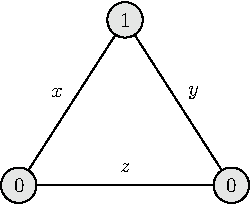
\includegraphics{../assets/742/triangle-1}%
    \caption{Labelled triangle graph.}
    \label{fig:tseitin-graph}
  \end{subfigure}
  \hfill
  \begin{subfigure}[b]{0.55\linewidth}
    \centering
    \begin{gather*}
      \begin{aligned}
	  & 
	  (x \lor y)
	  \\
	  \land \ 
	  &
	  (\olnot{x} \lor \olnot{y})
	  \\
	  \land \ 
	  &
	  (x \lor \olnot{z})
	  \\
	  \land \ 
	  &
	  (\olnot{x} \lor z)
	  \\
	  \land \ 
	  &
	  (y \lor \olnot{z})
	  \\
	  \land \ 
	  &
	  (\olnot{y} \lor z)
      \end{aligned}
    \end{gather*}
    \caption{Corresponding Tseitin formula.}
    \label{fig:tseitin-formula}
  \end{subfigure}
  \caption{Example Tseitin formula.}
  \label{fig:tseitin}
\end{figure}

 

When the maximal %
degree of $G$ is bounded by~$d$,
$\tseitinparity{v}{\tseitincharge}$ has
at most \mbox{$2^{d-1}$ clauses,}
all of width at most~$d$, and hence $\tseitinnot{G}{\tseitincharge}$ 
is a \mbox{$d$-CNF} formula with at most $2^{d-1} \setsize{V}$
clauses.
\Reffig{fig:tseitin-formula}
gives an example Tseitin formula generated from the graph in
\reffig{fig:tseitin-graph}.
%
We say that
%
a set~$U$ of vertices    %
has 
\introduceterm{odd (even) charge} if 
$\tseitincharge(U) = \sum_{u\in U} \tseitincharge(u)$ 
%
is odd (even, resp.).  %
By a simple counting argument one sees that
$\tseitinnot{G}{\tseitincharge}$ 
is unsatisfiable if
$\vertices{G}$
has odd charge.
%
Lower bounds on the hardness of
refuting such unsatisfiable formulas
$\tseitinnot{G}{\tseitincharge}$ 
%
can be proven in terms of the
connectivity  %
%
%
%
expansion of~$G$
as defined next.  

\begin{definition}[Connectivity expansion~\cite{ABRW02SpaceComplexity}]
  \label{def:connectivity-expansion}
  The \introduceterm{connectivity expansion} of $G=(V,E)$ is
  the largest $\connectivityexpansionnot$ such that for every
  $E'\subseteq E$, $\setsize{E'}\leq \connectivityexpansionnot$, the graph $G'=(V,E\setminus
  E')$ has a connected component of size strictly greater than
  $\setsize{V}/2$.
\end{definition}
%
%
%
%
%
%
%
%

%
%
%
%
%
%
%
%

\begin{definition}[Substituted formula]
  \label{def:substituted-formula}
If $F$ is a CNF formula over a set %
$X$ of variables  %
and
$\funcdescr{f}{\set{0, 1}^{\pebdeg}}{\set{0, 1}}$
is a Boolean function, then 
we can obtain a new CNF formula over a set
%
$X^{\pebdeg}$ of new variables  %
by
%
substituting $f(x_{i,1}, \ldots, x_{i,\pebdeg})$ for every variable~$x_i\in X$
%
%
%
%
and expanding out to conjunctive normal form. We write 
$\substform{F}{f}$   %
%
to denote the resulting \introduceterm{substituted formula}. %
\end{definition}
We will be
interested in substitutions with a
particular kind of functions defined as follows.

\begin{definition}[\Nonauthor{} function
  \cite{BN11UnderstandingSpace}]
  \label{def:nonauth-func}
  We say that
  a Boolean function $f(x_1, \ldots, x_{\pebdeg})$ is
  \introduceterm{\nonauthor{}} if for every
  variable~$x_i$ %
  and for every
  assignment $\alpha$ to
  $x_i$ there exist %
%
assignments  %
$\alpha_0, \alpha_1$
to $(x_1,\dots,x_{\pebdeg})$   %
%
%
%
%
extending $\alpha$ such that $f(\alpha_b) = b$ for $b \in \set{0, 1}$.
\end{definition}

By way of example, exclusive or (XOR), denoted~$\xor$, 
is clearly \nonauthor, since regardless of the
value of one variable, the other one can be flipped to make the
function true or false.  %
%
But standard (non-exclusive) or, $\lor$, is not non-authoritarian.  %
%
%
%
%

%
%
Let us finally give a brief overview of the framework developed
in~\cite{BG15Framework},
which we use to prove our PCR space lower bounds.%
%
%
%
%
%
%
\footnote{The definitions we use are equivalent in essence but not in detail to those in~\cite{BG15Framework}.
%
%
%
%
We prove that the same results still hold in
%
%
\refapp{sec:bg-framework}   %
    for completeness.}

A \introduceterm{partial partition}
$\partitionnot$ of a
%
set $V$ of variables  %
is a collection of disjoint %
subsets  %
$Q_i\subseteq V$. 
We use the notation $\Union \partitionnot =
%
%
\Union_{Q\in\partitionnot} Q$. %
For two sets of partial
assignments, $H$ and $H'$, %
to disjoint domains, we denote by $H \times H'$ the set of 
assignments %
%
%
%
defined by \[ H \times H' = \setdescr{\alpha \union
  \beta}{\alpha \in H \text{\ and\ } \beta \in H'} \eqperiod\] %
A set %
$H$ of partial assignments  %
to the %
%
set $Q$ of variables  %
is
\introduceterm{\flippable{}} on $Q$ if for each
variable $x \in Q$ and $b \in \set{0, 1}$ there exists an assignment
$\alpha_b \in H$ such that $\alpha_b(x) = b$. 
%
We say that
$H$ \introduceterm{satisfies} a formula $F$ if all 
$\alpha \in H$
%
satisfy $F$.

A \introduceterm{$\partitionnot$-structured assignment set} is a pair
$(\partitionnot, \assignmentsetnot)$ 
consisting of a partial partition $\partitionnot =
\set{Q_1, \ldots, Q_t}$ of $V$ and a set of 
partial assignments, %
$\assignmentsetnot = \prod_{i = 1}^t H_i$, where
%
%
$H_i$ is an assignment to $Q_i$ and is flippable on $Q_i$.  %
%
%
%
%
We write $(\partitionnot, \assignmentsetnot) \preccurlyeq
(\partitionnot', \assignmentsetnot')$ if $\partitionnot \subseteq \partitionnot'$
and $\restrict{\assignmentsetnot'}{\partitionnot} = \assignmentsetnot$, where
$\restrict{\assignmentsetnot'}{\partitionnot} = \prod_{Q_i \in \partitionnot} H'_i$. 
A structured assignment set $(\partitionnot, \assignmentsetnot)$
\introduceterm{respects} a CNF formula $F'$ if for every clause $C \in
F'$ either $\vars{C}\intersection \Union \partitionnot=\emptyset$ or
there is a set $Q \in \partitionnot$ such that $\vars{C}\subseteq Q$ and
$\assignmentsetnot$ satisfies $C$.

Expressed in this language, the key technical definition in 
\cite{BG15Framework}
is as follows.

\begin{definition}[\KextendibleNok family]
  \label{def:k-extendible}
  A non-empty family~$\kextendfamily$ of structured assignment sets
  $\structuredassignmentsnot$ is \introduceterm{\kextendible{}} for a CNF
  formula $F$ with respect 
  to a satisfiable $F' \subseteq F$ 
%
%
%
  if every $\structuredassignmentsnot \in \kextendfamily$
  satisfies the following conditions.
  \begin{description}
  \item[Size]%
%
    $\setsize{\partitionnot} \leq \kextendiblenot$.
  \item[\Respectfulness{}]
%
    $\structuredassignmentsnot$ respects $F'$.
  \item[\Restrictionpropname{}] 
%
    For every $\partitionnot' \subseteq \partitionnot$ the restriction
    $(\partitionnot', \restrict{\assignmentsetnot}{\partitionnot'})$ is in
    $\kextendfamily$.
  \item[\Extensionpropname{}]
%
    If $\setsize{\partitionnot} < \kextendiblenot$ then for every
    clause $C \in F\setminus F'$ there exists
    $\structuredassignmentsnot['] \in \kextendfamily$ such that 
    \begin{enumerate*}
    \item $\structuredassignmentsnot \preccurlyeq \structuredassignmentsnot[']$,
    \item $\assignmentsetnot'$ satisfies $C$, 
      and
    \item $\setsize{\partitionnot'} \leq \setsize{\partitionnot} + 1$.
    \end{enumerate*}
  \end{description}
%
  When $F' = \emptyset$, we simply say that $\kextendfamily$
    is \kextendible for~$F$.
%
%
%
%
%
%
%
%
%
%
%
%
%
%
%
%
%
%
%
%
%

\end{definition}

To prove PCR space lower bounds for a formula $F$, it is sufficient to
find an extendible family for~$F$.

\begin{theorem}[\cite{BG15Framework}]
  \label{th:space-lower-bound}
Suppose that $F$ is a CNF formula which has \akextendible
  family~$\kextendfamily$
  with respect to some $F'\subseteq F$. Then
  $\mspaceref[\pcrnot]{F}\geq \kextendiblenot/4$.
\end{theorem}

All space lower bounds presented in this paper are obtained in this
  manner, where in addition we always have
  $F' = \emptyset$.
 
%
\section{Overview of results and sketches of some proofs}
\label{sec:overview-results}

In this section, we give
%
a more detailed overview with formal statements of our
results, and also provide some proof sketches in order to convey the
main technical ideas.
As a general rule, the upper bounds we state are for polynomial
  calculus (PC) whereas the lower bounds hold for the stronger system
  polynomial calculus resolution (PCR).
  In fact, even more can be said: just as is the case in
  \cite{ABRW02SpaceComplexity,FLNRT15SpaceCplx,BG15Framework},
  %
  all our lower bounds
  hold also for
  \introduceterm{functional calculus},
  where proof lines are arbitrary Boolean functions over
  clauses/monomials and anything that follows semantically from the
  current configuration can be derived in a single step. We do not
  discuss this further below but instead refer to
 \refapp{sec:bg-framework}
  for the details.


\mysubsection{Relating PCR space and resolution width}
\label{sec:width-monomialspace}

The starting point of our work is the question of how space and degree
are related in polynomial calculus, and in particular whether it is
true that degree %
%
%
is a lower bound on space.  %
%
%
While an exact characterization remains
open, we make partial progress by showing that if the resolution width
of refuting a CNF formula~$F$ is large (which in particular must be
the case if $F$ requires high degree), then by making XOR
substitution we obtain a formula
$\substform{F}{\xor}$
that requires
large PCR space.
In fact, this works not only for exclusive or but for any
\nonauthor function
(as defined in \refdef{def:nonauth-func}).
The formal statement
%
is as follows.


\begin{theorem}
  \label{thm:substitution}
  Let $F$ be a $\fkwidth$-CNF formula
  and let $f$ be any
  \nonauthor{} function. 
  Then it  holds over any field that
  $\mspaceref[\pcrnot]{\substform{F}{f}}
  \geq
  (\widthref[\resnot]{F} -  \fkwidth  + 1) /  4$.

\end{theorem}

\begin{ourproof}[sketch]
  In one sentence, the proof of
 \refth{thm:substitution} 
  is by combining the concept of
  \kextendibleNok families in
 \refdef{def:k-extendible}
  with the combinatorial  characterization of resolution width in~%
  \cite{AD08CombinatoricalCharacterization}.
  We show that the  properties of~$F$ implied by the
  width lower bound  can be used to construct an \kextendibleNok family for~%
  $\substform{F}{f}$.
  To make this description easier to parse,
  let us start by describing in somewhat more detail the width
  characterization in~%
  \cite{AD08CombinatoricalCharacterization}.
  
  Consider the following game played on~$F$
  by two players, %
  \introduceterm{Spoiler} and \introduceterm{Duplicator}. 
  %
  Spoiler asks about values assigned to variables in~$F$ and
  Duplicator answers true or false. Spoiler can only remember 
  $\adpebblenumber$~values
  simultaneously, however, and has to forget some variable when this limit is 
  reached.
  If Duplicator is later asked about some forgotten variable,
  the new value needs not be consistent with the previous
  forgotten one. Spoiler wins the game by constructing a partial
  assignment that falsifies some clause in~$F$, and
  %
  %
  Duplicator wins 
  if %
  Duplicator has  %
  a strategy to keep playing forever without
  Spoiler ever reaching this goal. It was proven in
  \cite{AD08CombinatoricalCharacterization}
  that this game exactly captures resolution
  width in the sense that Duplicator has a winning strategy if and only if
  $\adpebblenumber \leq \widthref[\resnot]{F}$.

  %
  %
  %
  Continuing our proof sketch, let us fix
  $\kextendiblenot=\widthref[\resnot]{F} - \fkwidth + 1$
  and  use Duplicator's winning strategy for
  $\adpebblenumber = \widthref[\resnot]{F}$
  to build \akextendible family for~%
  %
 %
  $F[\xor]$.  (The proof  %
  for general \nonauthor{} functions is very similar and is given in
   \refsecapp{sec:substitution}.)   %
  Consider any assignment $\alpha$ reached during the
  game. We define a corresponding structured assignment set
  $\structuredassignmentsnot[_\alpha]$
  by adding a block
  $Q_{x}=\set{x_{1},x_{2}}$
  to~%
%
  $\partitionnot_\alpha$
  for every $x \in \domainof{\alpha}$,
  %
  and let $H_{x}$ 
  contain all assignments~$\alpha_x$ to
  $\set{x_{1},x_{2}}$
  such that
  $\alpha_x (x_1 \xor x_2)  =  \alpha(x)$.
  %

  In the end the \kextendible family for $F[\xor]$ is built as the set
  of all $\structuredassignmentsnot[_\alpha]$ corresponding to the partial
  assignments $\alpha$ reached during the game played on $F$.
  %
  It only remains to verify that this construction yields indeed an
  \kextendibleNok family as described in \refdef{def:k-extendible},
  and to apply \refth{th:space-lower-bound}.
\end{ourproof}

\mysubsection{Separation of size and degree from space}
\label{sec:overview-separation}

An almost immediate consequence of \refth{thm:substitution} is that
there are formulas which have small PC refutations in constant
degree but nevertheless require maximal space in PCR.

\begin{theorem}
  \label{thm:separation}
%
  For any field $\fieldstd$
  of characteristic~$p>0$
  there is a family of
  \mbox{$\fkwidth$-CNF} formulas
  $F_n$
  (where $\fkwidth$ depends on~$p$)
  of size $\bigoh{n}$
  for which
%
  $\mspaceref[\pcrnot]{F_{n}}=\bigomega{n}$
  %
  %
  over any field~$\fieldstd'$ %
  but  which have tree-like PC refutations
  $\refof{\proofstd_n}{\fstd_n}$ 
  over~$\fieldstd$
  of size
  $\sizeofarg{\proofstd_n}=\bigoh{n\log n}$
  and degree
  $\mdegreeof{\proofstd_n}=\bigoh{1}$.
\end{theorem}


\begin{ourproof}[sketch]
  Let us focus on 
  $p=2$, deferring the general proof to  
   \refsecapp{sec:tseitinseparation}.
  Consider a Tseitin formula $\tseitinnot{G}{\tseitincharge}$ 
  for any constant-degree graph~$G$ over $n$~vertices
  with connectivity expansion $\bigomega{n}$
  and any odd-charge function~$\tseitincharge$.
  
  From~\cite{BW01ShortProofs}
  we know that
  $\widthref[\resnot]{F}=\bigomega{n}$.
  It is not hard to see that XOR substitution yields
  another Tseitin formula
  $\tseitinnot{G'}{\tseitincharge}$ 
  for the multi-graph $G'$ obtained from $G$ 
  by adding double copies of all edges.
  This formula requires large PCR space (over any field)
  by \refth{thm:substitution}.
  The upper bound follows by observing that the CNF encodes a linear
  system of equations, which is easily shown inconsistent in PC by summing
  up all equations in a tree-like fashion.
\end{ourproof}

It follows from \refth{thm:separation} that
tree-like space in PC/PCR is not %
a lower bound on the logarithm of %
tree-like size, in contrast to resolution. 
This is the only example we are aware of where the relations between
size, degree, and space in PC/PCR differ from those between length,
width, and space in resolution, so let us state this as a formal
corollary.


\begin{corollary}
  \label{cor:no-space-leq-log-length-bounf}
  It is \emph{not true} in PC/PCR
  that tree-like space complexity is %
  a lower bound on 
  the logarithm of tree-like size complexity.
\end{corollary}

\mysubsection{Space complexity of Tseitin formulas} 
\label{sec:tseitin-overview}

A closer analysis of the proof of
\refth{thm:separation}
reveals that it partitions the edge set of~$G'$
into %
short  %
edge-disjoint cycles (namely, \mbox{length-$2$} cycles 
corresponding to the two copies of each original
edge) and uses partial assignments
%
that all maintain the same parities of the vertices on a given
cycle. It turns out that this approach can be made to work in
greater generality as stated next.

\begin{theorem}
  \label{th:tseitin-small-cycles-space-lower-bound}
  Let $G = (V,E)$ be a
  connected
  %
  graph of %
  maximal degree~$d$  %
  %
  %
  with connectivity expansion $\connectivityexpansionnot$ such that 
  the edge set~$E$ can be partitioned into
  %
  cycles of length at most~$\cyclelengthnot$.
  Then it holds over any field that
  $
  \mspaceref[\pcrnot]{\tseitinnot{G}{\tseitincharge}}\geq
  \connectivityexpansionnot/4\cyclelengthnot -d/8 
  $.
\end{theorem}

\begin{ourproof}[sketch]
%
%
  We build on the
  resolution space lower bound in~%
  \mbox{\cite{ABRW02SpaceComplexity,ET01SpaceBounds},}
  where the proof works by inductively constructing an assignment
  $\alpha_t$ for
  each derived configuration $\clsc_t$
  (which corresponds to removing edges 
  from~$G$
%
  and updating the vertex
  charges accordingly) such that
  (a)~$\alpha_t$ satisfies $\clsc_t$, and  
  (b)~$\alpha_t$~does not create any odd-charge component in~$G$ of 
  size less than~$n/2$.
  The inductive update 
  can be performed 
%
  as long as the space is not too large,
  which shows that contradiction cannot be derived in small space
  (since $\clsc_t$ is satisfiable).

  To lift this proof to PCR, however, 
%
  we must maintain not just one but an exponential number of such good
  assignments, and in general we do not know how to do this.
  Nevertheless, some more thought reveals that the only important
  aspect of our assignments are the resulting vertex parities.
  And if the edge set is partitioned into cycles, we can always shift
  edge charges along the cycles so that for all the exponentially many
  assignments,  
  the vertex parities
  are all the same (meaning 
  that on a higher level
  we only have to maintain one good assignment after  all). 
%
  The full proof is presented in \refsecapp{sec:small-cycles}.
\end{ourproof}

Some graphs, such as rectangular grids, can be partitioned into cycles
of size~$\bigoh{1}$, yielding tight bounds on space.
A bit more surprisingly, random \mbox{$d$-regular} graphs for $d \geq 4$ turn out to
(sort of)
admit partitions into cycles of %
length
$\bigoh{\sqrt{n}}$,
which yields the following theorem.

\begin{theorem}
  \label{thm:improved-general}
  Let $G$ be a random $d$-regular graph on $n$~vertices, where $d\geq 4$.
  Then over any field it holds almost surely that
  $\mspaceref[\pcrnot]{\tseitinnot{G}{\tseitincharge}} = \Bigomega{\sqrt{n}}$.
\end{theorem}

\begin{ourproof}[sketch]
  As long as we are interested in properties holding asymptotically
  almost surely, we can replace random $4$-regular graphs with unions
  of two random Hamiltonian cycles~\cite{KW}.
  We show that a graph distributed according to the latter
  model almost surely decomposes into cycles of length
  $\bigoh{\sqrt{n}}$, along with $\varepsilon n$ additional edges 
  (which are easily taken care of separately).
  Since random graphs are also excellent expanders, we can
  apply 
 \refth{th:tseitin-small-cycles-space-lower-bound}.
  The argument  
  extends straightforwardly
  to random $d$-regular graphs for any 
  $d  \geq 4$.
  The full proof, which contains a bit more by way of technical
  details, is  given in
 \refsecapp{sec:cycle-partitions}.
\end{ourproof}

%
We 
%
believe that the true space bound should actually be
$\bigtheta{n}$, just as for resolution, but such a result seems beyond
the reach of 
our current techniques.
%
Also, note that to make
\refth{th:tseitin-small-cycles-space-lower-bound}
go through we need graph expansion
\emph{plus}
partitions into %
short cycles.
%
It seems 
%
plausible that expansion alone should 
be enough to imply
linear PCR space lower bounds, as for resolution, but again
we are not able to prove this.
In a recent paper, Galesi \etal~\cite{GKT19SpaceWidth}
  prove a space lower bound just using graph expansion, with no need
  for a partition into %
  short cycles to exist, but interestingly they
  obtain a $\bigomega{\sqrt{n}}$ space lower bound as well.


%
\mysubsection{Limitations of the PCR space lower bound technique}
\label{sec:space-compl-funct}


The framework in~\cite{BG15Framework} can also be used to
rederive all PCR space lower bounds shown previously 
in~\cite{ABRW02SpaceComplexity,FLNRT15SpaceCplx}, and in this sense
\cite{BG15Framework} 
sums up what we knew about PCR space lower bounds up to that point.
There are also intriguing similarities between~%
\cite{BG15Framework} 
and the resolution width characterization 
  in~\cite{AD08CombinatoricalCharacterization}
(as partly hinted in the proof sketch for
\refth{thm:substitution}),
which raises the question whether
\kextendibleNok families 
could perhaps be a step towards
characterizing degree and showing that degree
%
%
is a lower bound on  %
%
%
space in PC/PCR.

Even more intriguingly, there are CNF formulas for which
\kextendibleNok families are hard but possible to construct, such as
random $3$-CNF formulas~\cite{BBGHMW17SpaceProofCplx}, and formulas
where \kextendibleNok families seem very hard to construct. Such
formulas include ordering principle formulas, for which PCR space
lower bounds are expected to hold, and functional pigeonhole principle
(FPHP) formulas, for which (possibly not tight) PCR space lower bounds
can be proven by other means~\cite{GKT19SpaceWidth}.

We show that the problems in applying~%
\cite{BG15Framework}
to the functional version of the pigeonhole principle are inherent, 
in that these techniques provably cannot establish
%
\emph{any} nontrivial
space lower bound.
%
We refer to
 \refsec{sec:limitations}
%
  for the formal description of the formulas
  and
%
%
%
  the proof of the 
  next theorem.

\begin{theorem}
  \label{th:no-kextendible}
  There is no \kextendible family for
  $\fphpnot{n+1}{n}$ 
%
  for
  $\kextendiblenot>1$. 
\end{theorem}
  
%
%
%
%
%
%
%
%
%
%
%
%
%
%
%
%
%
%
%
%
%
%
%
%
%
%
%
%
%
%
%

Since by~\cite{Razborov98LowerBound,MN15GeneralizedMethodDegree}
these formulas
require PC refutation
degree $\bigomega{n}$, one way of interpreting
\refth{th:no-kextendible} is that the concept of \kextendible families
is very far from providing the hoped-for characterization of degree.
%
That is a pity since in principle the framework
in~\cite{BG15Framework} allows to show space lower bounds up to linear
size, while the technique in~\cite{GKT19SpaceWidth} cannot.

One step towards proving linear space lower bounds for PCR could be to
obtain a weaker linear space lower bound for PC---as noted above in
the discussion of \mbox{$3$-CNF} formulas, this can sometimes
be easier.
%
For
$\fphpnot{n+1}{n}$,
%
however,
and for a slightly more general class of formulas
described in
 \refsec{sec:limitations},
%
%
%
%
it turns out that the monomial space is more or less the same
between PC and PCR.

%

\begin{theorem}\label
  {th:fphppcequalpcrspace}
  $\mspaceref[\pcrnot]{\fphpnot{n+1}{n}}
  =
  \bigtheta{\mspaceref[\pcnot]{\fphpnot{n+1}{n}}}$.
%
%
%
%
\end{theorem}


\begin{ourproof}[sketch]
  In
%
  $\fphpnot{n+1}{n}$
  we have variables
  $x_{i,j}$
  for
%
  $i \in \numset{n+1}$,
  $j \in \numset{n}$,
%
  encoding that pigeon $i$ goes into hole~$j$. The clauses of the
  formula require that every pigeon is mapped to some hole and that
  this mapping is one-to-one.
  Because of this, the negation of
  $x_{i,j}$
  is equivalent to 
  $\Lor_{j'\neq j} x_{i,j'}$
  and so the literal
  $\olnot{x}_{i,j}$
  can be encoded as the monomial
  $\prod_{j'\not=j} x_{i,j'}$
  in PC.
  Since this substitutes a monomial for a monomial the space does not
  increase. 
  Now we can take any PCR refutation of
  $\fphpnot{n+1}{n}$
%
  and apply such substitutions line by line.
  The inferences remain sound (with some local auxiliary steps added)
  and so this process gives a PC refutation of
  $\fphpnot{n+1}{n}$ 
%
  in roughly the same space.
%
%
%
%
%
%
%
%
%
\end{ourproof}

 
%
\section{PCR space lower bounds from resolution width}%
%
\label{sec:substitution}

In the rest of this paper, 
we give formal proofs of the results described in
\refsec{sec:overview-results}.
We start by considering  the question of relating space and degree
in PCR\@. Although we do not know how to prove (or rule out) an analogue
of the relation between space and width in resolution, 
we can use the combinatorial game from
\cite{AD08CombinatoricalCharacterization} 
to prove a weaker relation between PCR space and resolution width. Recall
from the informal description of the game in
\refsec{sec:width-monomialspace} that we have two players, Spoiler and
Duplicator, and that Duplicator needs to be able to provide an
answer to any of Spoiler's questions about assignments to some
bounded number of variables in order to win the game. Formally, a
winning strategy for Duplicator is defined as follows.

\begin{definition}[Duplicator's strategy
  \cite{AD08CombinatoricalCharacterization}]
  \label{def:AD-game}  
%
%
%
%
%
%
%
%
  A
  \introduceterm{Duplicator winning strategy}
  for the Boolean existential $\adpebblenumber$-pebble game on 
  a CNF formula~$F$ is a non-empty family $\adduplicatorfamily$ of
  partial truth value assignments 
%
  to $\vars{F}$
  such that every 
  $\alpha \in \adduplicatorfamily$ 
  satisfies the following conditions:
  \begin{enumerate}
  \item
    No clause $\clc \in F$ is falsified by~$\alpha$.
  \item
    The domain of $\alpha$ has size at most
    $\setsize{\domainof{\alpha}} \leq \adpebblenumber$.
  \item 
    For every 
    subassignment
    $\alpha' \subseteq \alpha$ 
    it holds that
    $\alpha' \in \adduplicatorfamily$.
%
%
%
%
  \item 
    If $\setsize{\domainof{\alpha}} < \adpebblenumber$, then for every
    variable $x$ there exists an $\alpha' \in \adduplicatorfamily$ 
    that assigns a value to~$x$
    and extends $\alpha$ 
    (\ieComma $\alpha' \supseteq \alpha$).
%
%
%
%
  \end{enumerate}
\end{definition}

In \cite{AD08CombinatoricalCharacterization}, Atserias and Dalmau
proved the following tight connection between Duplicator winning strategies 
and resolution refutation width.
%
%

\begin{theorem}[\cite{AD08CombinatoricalCharacterization}]
  \label{th:ADWidthCharacterization}
%
%
%
  The CNF formula~$F$ has a resolution refutation of width
  $\adpebblenumber$ if and only if Duplicator has no winning strategy
  for the Boolean existential $(\adpebblenumber + 1)$-pebble game on $F$.
\end{theorem}

%
%
%
%
%
%
%
%
%
%
%
%
%
%
%
%

The Duplicator strategy in \refdef{def:AD-game} has some similarities
with the \kextendibleNok{} family in \refdef{def:k-extendible}, which
can be taken to suggest that there might be a relation between
resolution width and PCR space. The main difference is that
\kextendibleNok families consist of sets of assignments in
which we must be able to flip every variable, while Duplicator's
strategy is built on fixed individual assignments. However,
if we substitute every variable in~$F$ with a \nonauthor{} function as
defined in \refdef{def:nonauth-func}, then it is straightforward to
make the transition from fixed assignments to sets of \flippable assignments.
%
%
%
%
%
%
%


\begin{lemma}
  \label{lem:substitution}
  Let $F$ be a $\formulakwidth$-CNF formula and let $f$ be a
  \nonauthor{} function.
  %
%
  If Duplicator wins the
  Boolean existential $\adpebblenumber$-pebble game on $F$, then there
  exists an $(\adpebblenumber - \formulakwidth + 1)$-\kextendibleNok{}
  family for 
%
  $\substform{F}{f}$.
%
%
%
\end{lemma}

\begin{proof}
  Let $\adduplicatorfamily$ be a winning Duplicator strategy for~$F$. 
  %
  We will use 
  $\adduplicatorfamily$
  to construct an 
  $(\adpebblenumber - \formulakwidth + 1)$-\kextendibleNok family 
  $\kextendfamily$ for the substituted formula
  $\substform{F}{f}$. 
  In what follows, let us denote by
  $\variablecopies{x}$ 
  the set of
  variables that we get when we substitute $x$ by 
  $f (x_1, \ldots, x_{\farity})$ in $F$ 
  for some \nonauthor function $f$ of arity~$\farity$.

%
%
%
%
%
%
%
%
%
%
%
%
%
%
%
%
%
%
%
%
%
%
%
%
%
%
%

  For $x \in \vars{F}$,
  define
  $Q_x = \variablecopies{x}$
  and let
  $H_{x,\alpha} = 
  \setdescr{\beta}{\domainof{\beta} = Q_x \text{ and } f(\beta) = \alpha(x)}
%
%
  $
  be the set of all assignments over
  $Q_x$ for which $f$ evaluates to the value that $\alpha$ assigns to $x$.
  For any partial assignment 
  $\alpha \in \adduplicatorfamily$
  we let the corresponding structured assignment set
  $\structuredassignmentsnot[_\alpha]$ be the pair 
  consisting
  of $\partitionnot_\alpha =
  \setdescr{Q_x}{x \in \domainof{\alpha}}$ 
  and 
  $\assignmentsetnot_\alpha = \prod_{x \in \domainof{\alpha}} H_{x,\alpha}$.
  We define $\kextendfamily$ to encompass all
  structured assignment sets 
  $\structuredassignmentsnot[_\alpha]$ 
  corresponding to partial assignments 
  $\alpha \in \adduplicatorfamily$
  with 
  $\setsize{\domainof{\alpha}} \leq \adpebblenumber - \formulakwidth + 1$.
  We need to prove that
  $\kextendfamily$ 
  constructed in this way is an 
  $(\adpebblenumber - \formulakwidth + 1)$-\kextendibleNok 
  family with respect to 
  $F' = \emptyset$. 
  
%
%
%
%
%
%
%
%
%
%
%
%
  By construction, for every
  $\structuredassignmentsnot[_\alpha] \in \kextendfamily$
  we have that 
  $\partitionnot_\alpha$ 
  is a partial partition and that the partial assignments
  $H_{x,\alpha} \in \assignmentsetnot_\alpha$ 
  assign to 
  $Q_x \in \partitionnot_\alpha$.
  Furthermore, 
  $H_{x,\alpha}$ is \flippable on $Q_x$.
  This is so since 
  $f$ is a \nonauthor{} function, which means that 
%
%
  for very variable in~$x_i \in Q_x$
  there exist assignments~$\beta_b$, $b \in \set{0,1}$,
  to~$Q_x$
  such that $\beta_b(x_i) = b$
  and
  $f(\beta_b) = \alpha(x)$.
  Hence, all  
  $\structuredassignmentsnot[_\alpha] \in \kextendfamily$
  are structured assignment sets.


  The size condition
  $\setsize{\partitionnot_\alpha} \leq  \adpebblenumber - \formulakwidth + 1$ 
  in
 \refdef{def:k-extendible}
  is clearly satisfied for all
  $\structuredassignmentsnot[_\alpha] \in \kextendfamily$, 
  and \respectfulness is vacuously true.
  To see that the \restrictionproperty{} also holds,
%
%
%
  consider any
  \mbox{$\structuredassignmentsnot[_\alpha] \in \kextendfamily$} 
  obtained from $\alpha \in \adduplicatorfamily$.
  For any subset 
  $\partitionnot' \subseteq \partitionnot_\alpha$, 
  let
  $\alpha'$
  be the subassignment of 
  $\alpha$
  restricted to 
  $\setdescr{x}{Q_x \in \partitionnot'}$
%
  and let
  $
  \assignmentsetnot' = 
  \prod_{Q_x \in \partitionnot'} H_{x,\alpha} =
  \prod_{x \in \domainof{\alpha'}} H_{x,\alpha'}
  $.
  Then since
  $\alpha' \in \adduplicatorfamily$
  by
 \refdef{def:AD-game},  
  it follows by the construction of~$\kextendfamily$
  that
  $
  (\partitionnot', \restrict{\assignmentsetnot}{\partitionnot'})
  =
  \structuredassignmentsnot[']
  \in
  \kextendfamily$
  as required.
%
%
%
%
%
%
%
%
%
%
%
%


  It 
%
  remains to prove that $\kextendfamily$ has the
  \extensionproperty{}. 
%
%
%
%
%
%
%
  Let $\structuredassignmentsnot[_\alpha] \in \kextendfamily$ be 
  such that
  $\setsize{\partitionnot_\alpha} < \adpebblenumber - \formulakwidth + 1$ 
  and
%
  let 
  $C$ be a clause in~$\substform{F}{f}$.
  We need to argue that 
  $\structuredassignmentsnot[_\alpha]$
  can be extended to satisfy~$C$.
%
  Let 
  $A \in F$
  be the clause such that
  $C \in \substform{A}{f}$,
  \ieComma $C$ is one of the clauses
  obtained when substituting
%
  $f$ in~$A$. 
  If
  $\alpha \in \adduplicatorfamily$ 
  satisfies~$A$, it follows by construction that 
  $\assignmentsetnot_\alpha$
  satisfies all of 
  $\substform{A}{f}$ 
  and hence, in particular,~$C$, and we are done.
  Otherwise, 
%
%
%
%
%
%
%
%
  it follows
  from the definition 
  of a winning Duplicator strategy and the
  fact that $\setsize{\alpha} \leq \adpebblenumber - \formulakwidth$
  that $\alpha$ can be extended to an assignment $\alpha'$
%
%
%
  that queries all of the (at most~$\formulakwidth$) variables in~$A$ 
  without falsifying the clause. Such an $\alpha'$ must satisfy~$A$.
  Fix some variable
  $x^* \in \domainof{\alpha'} \setminus \domainof{\alpha}$
  such that $\alpha'$ satisfies $A$ by assigning to $x^*$,
  and let
  $\alpha^*$ be the subassignment of $\alpha'$
  with domain
  $\domainof{\alpha} \union \set{x^*}$.
%
%
%
%
%
%
%
%
%
%
%
%
%
%
%
  This $\alpha'$ must be in $\adduplicatorfamily$ by
 \refdef{def:AD-game},  
  and analogously to what was argued above it must hold that
  $\assignmentsetnot_{\alpha^*}$
  satisfies~$C \in \substform{A}{f}$.
  It is clear that
  $\structuredassignmentsnot[_{\alpha}] 
  \preccurlyeq 
  \structuredassignmentsnot[_{\alpha^*}]$,
  and that
  $\setsize{\partitionnot_{\alpha^*}} \leq
  \setsize{\partitionnot_\alpha} + 1$.
  Hence, 
  $\kextendfamily$ satisfies
  \extensionpropname, and the lemma follows.
\end{proof}

Combining \reflem{lem:substitution}
with the combinatorial characterization of width in~%
\refth{th:ADWidthCharacterization} 
and the lower bound on space in terms of \kextendibleNok families in~%
\refth{th:space-lower-bound},
we obtain the first theorem claimed in 
\refsec{sec:overview-results}.


%
%
%
%
\begin{theorem}[restatement of \expref{Theorem}{thm:substitution}]
%
  Let $F$ be a $\formulakwidth$-CNF formula and let $f$ be any
  \nonauthor{} function. Then
  it holds over any field that %
  \begin{equation*}
    \mspaceref[\pcrnot]{\substform{F}{f}} 
    \geq 
    \frac{\widthref[\resnot]{F} - \formulakwidth + 1}{4} \eqperiod
  \end{equation*}
  %
%
\end{theorem}

While it can be argued that this theorem might be interpreted as an
indication that degree could be a lower bound for space in PCR, a more
immediate and concrete consequence is that 
it gives us a way to prove the existence of formulas which have very
small PCR refutations, but for which any refutation must
have essentially maximal space. 
%
For polynomial calculus over fields of characteristic~$2$, we already
have all the tools needed to argue this. In particular, 
the space lower bound needed
follows immediately from
\refth{thm:substitution}
as described next.

\begin{corollary}\label{cor:tseitin-double}
  Let $G$ be
%
%
  an expander graph of bounded maximal %
  degree over $n$~vertices,
  let
  $\tseitincharge$ be an odd-charge function on 
  $\vertices{G}$,
  and let $G'$ be 
  %
  the multi-graph obtained by adding two copies of each edge in~$G$.
  %
%
  Then
  \begin{equation*}
    \mspaceref[\pcrnot]{\tseitinnot{G'}{\tseitincharge}} =
    \bigomega{n}
    \eqperiod
  \end{equation*}
\end{corollary}
\begin{proof}
  As shown in~\cite{BW01ShortProofs},
  refuting Tseitin formulas over expander graphs requires linear width
  in resolution. It is not hard to see that substituting with XOR in a
  Tseitin formula over $G$ is the same as considering 
  the formula over the multi-graph with two copies of every edge.
  %
  Thus~$\tseitinnot{G'}{\tseitincharge}$ requires monomial space
  $\bigomega{n}$ 
  by
 \refth{thm:substitution},
  which is linear in the formula size if $G$ is a constant-degree expander.
\end{proof}

As briefly discussed in 
\refsec{sec:overview-separation}, 
it is not hard to show that Tseitin formulas have small 
refutations in PCR (and even PC) over fields of characteristic~$2$,
which yields
\refcor{cor:no-space-leq-log-length-bounf} 
for this characteristic. 
However, this upper bound does not hold for characteristics distinct
from~$2$. 
%
Therefore, we need to work with generalized version of Tseitin formulas
and prove our results for such formulas instead. We do so in the next section.
%

\section{Formulas with small proofs may require large space}
\label{sec:tseitinseparation}

In \expref{Section}{sec:preliminaries} we defined Tseitin formulas as the
CNF encoding of particular linear systems over $\fieldstd_{2}$.  Here we
consider a generalization over fields of any positive characteristic.
%
Any such formula essentially defines an unsatisfiable linear system over
$\fieldstd_{p}$ for some prime $p$. In order to efficiently encode this
linear system as a CNF it is important that each equation mentions a
small (\egComma constant) number of variables: any equation over $d$
variables can be encoded as a set of at most $2^{d}$ clauses with $d$
literals each.  In particular, Tseitin formulas are defined on
directed graph as follows.

\begin{definition}\label{def:tseitinmodp}
  Let $G = (V,E)$ be a directed graph and
  $\funcdescr{\tseitincharge}{V}{\fieldstd_p}$
  be a function.
  Identify every directed edge $(u,v) \in E$ with a variable $x_{(u,v)}$
  and  let
  $\tseitinmodpflow{v}{\tseitincharge}$
  denote the CNF encoding
  of the constraint
  that the number of \emph{incoming} edges~$x_{(u,v)}$ incident to a vertex $v \in V$ that are set to true, minus the number of \emph{outgoing} edges~$x_{(v,w)}$ set to true is equal to $\tseitincharge(v) \pmod{p}$.
  Then the \introduceterm{Tseitin formula} over~$G$ \wrt{}~$\tseitincharge$
  is $\tseitinmodpnot{G}{\tseitincharge}=
  \bigwedge_{v\in V}\tseitinmodpflow{v}{\tseitincharge}$.
\end{definition}

This formula is unsatisfiable when $\sum_{v}\tseitincharge(v)\not\equiv 0
\pmod{p}$. Compare \refdef{def:tseitinmod2} with
\refdef{def:tseitinmodp}: for $p=2$ the definitions
coincide because in such characteristic there is no difference
between the contribution of the incoming and the outgoing edges. For
$p=2$ it is natural to define the formula in terms of undirected
graphs, indeed.
%
Not surprisingly, polynomial calculus over a field of characteristic
$p$ efficiently refutes unsatisfiable Tseitin formulas defined on
sums modulo $p$.

\begin{lemma}\label{lmm:tseitinupperbound}
  Consider a directed graph $G=(V,E)$ with $n$ vertices and constant
  degree, and a function
  \mbox{$\funcdescr{\tseitincharge}{V}{\fieldstd_p}$}
  with
  $\sum_{v}\tseitincharge(v)\not\equiv 0 \pmod{p}$. The formula
  $\tseitinmodpnot{G}{\tseitincharge}$ has a tree-like polynomial calculus
  refutation of constant degree, size $\bigoh{n\log n}$, and monomial
  space $\bigoh{n}$.

  Furthermore, given any boolean function $f$ on a constant number of
  variables, the result holds for the substituted formula
  $\substform{\tseitinmodpnot{G}{\tseitincharge}}{f}$.
\end{lemma}

\begin{proof}
Let us first consider the case without substitution. Recall that true value is encoded as $0$ and false as 1. In this encoding formula $\tseitinmodpflow{v}{\tseitincharge}$ is equivalent to
  \begin{equation}\label{eq:tseitinequations}
    \sum_{u\colon(u,v)\in E} (1-x_{uv}) - \sum_{w\colon(v,w)\in E} (1-x_{vw})
    \equiv \tseitincharge(v) \pmod{p} \eqperiod
  \end{equation}

  The proof is based on the natural intuition that summing the
  equations~\eqref{eq:tseitinequations} for all vertices in the graph
  results in a contradiction, since in the sum each variable appears
  twice: once with positive and once with negative sign.
  %
  Fix an enumeration of $V=\{v_{1},\ldots
  v_{n}\}$, and fix the following notation for partial sums:
  \begin{equation}
    S_{a,b}:=
    \sum^{b}_{i=a}
    \left[\sum_{u:(u,v_{i})\in E} (1-x_{uv_{i}})
    -
    \sum_{w:(v_{i},w)\in E} (1-x_{v_{i}w})\right]
    \equiv
    \sum^{b}_{i=a} \tseitincharge(v_{i}) \pmod{p} \eqperiod
  \end{equation}
  
  %
  %
  
  We fix $t=2^{\lceil \log n \rceil} < 2n$ and consider $S_{i,i}$ to
  be the equation ``$0=0$'' for all $n < i \leq t$.
  %
  We set up a tree of height $\lceil \log n \rceil$, where leaves are
  labeled by equations $S_{i,i}$ and internal nodes are labeled by the
  sum of the two children labels (\ieComma a node at level $k$ is labeled
  by the equation $S_{i,i+2^{k}-1}$ for some $i$).

  Each equation $S_{i,i}$ is derived from the encoding of
  $\tseitinmodpflow{v_{i}}{\tseitincharge}$. This equation mentions only a constant
  number of variables, so by implicational completeness of polynomial
  calculus (see \expref{Lemma}{lmm:pccompleteness}) we have a derivation
  of constant space and size.

  Equations in internal nodes are derived by summing the
  equations of the children. We derive all the equations of the tree
  in a bottom-up fashion. This concludes the refutation since the
  equation $S_{1,t}$ at the root is
  \begin{align}
    \sum^{n}_{i=1}
    \left[
    \sum_{u:(u,v_{i})\in E} (1-x_{uv_{i}}) -\sum_{w:(v_{i},w)\in E} (1-x_{v_{i}w})
    \right]
    & \equiv \sum^{n}_{i=1} \tseitincharge(v_{i}) \pmod{p}
    \\
    \sum_{(u,v)\in E} (1-x_{uv}) -\sum_{(v,w)\in E} (1-x_{vw})
    & \equiv \sum^{n}_{i=1} \tseitincharge(v_{i}) \pmod{p}\\
    0 \equiv \sum^{n}_{i=1} \tseitincharge(v_{i}) \pmod{p}
  \end{align}
  Which is the end of the refutation, since $\sum^{n}_{i=1} \tseitincharge(v_{i})$
  is non-zero.

  The size of the proof accounts $\bigoh{1}$ for the deduction of each $S_{i,i}$, and $\bigoh{n}$ for the total number of monomials at each level of the tree: at level $k$ there are $\frac{t}{2^{k}}$ equations with at most  $\bigoh{2^{k}}$ monomials. So the total size is as claimed.

  Regarding the monomial space, notice that we need to keep simultaneously in memory only the equations of two adjacent levels, which have at most $\bigoh{n}$ monomials.

  The degree of the refutation is $\bigoh{1}$ for the inference of each equation $S_{i,i}$. The rest of the proof has degree $1$.

  The case with substitution is similar: consider a substituting
  function $f$ on a constant number of variables. There is a
  multilinear polynomial $p_{f}$ which evaluates exactly as $f$ on all
  $\{0,1\}$ inputs, and which mentions a constant number of monomials.

  The substituted linear forms $\substform{S_{i,i}}{f}$ are linear
  combinations of copies of $p_{f}$, so they have a constant
  number of variables each and their inference from
  $\substform{\tseitinmodpflow{v_{i}}{\tseitincharge}}{f}$ is doable in constant
  space, size and degree because of~\reflem{lmm:pccompleteness}.

  Once the equations $\substform{S_{i,i}}{f}$ are derived, the
  refutation goes exactly as shown for the case with no
  substitution. From this point on the original refutation is linear;
  applying the trivial substitution to these proof lines increases the
  space, degree and size only by constant factors.
\end{proof}

For the sake of self-containment, we give a proof of the
implicational completeness of polynomial calculus. This completes the proof
%
of \reflem{lmm:tseitinupperbound}.    %

\begin{lemma}\label{lmm:pccompleteness}
  Consider a polynomial implication $p_{1}, \ldots, p_{l}\models p$ which is valid over $\{0,1\}$ assignments. Assume all involved polynomials collectively mention $d$ variables and have degree $\bigoh{d}$; then there is a PC proof of this implication in degree $\bigoh{d}$, space $2^{\bigoh{d}}$, and size $2^{\bigoh{d}}$.
\end{lemma}
\begin{proof} Without loss of generality we assume that all
  polynomials are in multilinear form. This is because we can
  transform any polynomial of degree $\bigoh{d}$ between its original
  and multilinear version in size and space $2^{\bigoh{d}}$. So each
  of the polynomials has size at most $2^{d}$ and degree $d$.
  %
  Let $\alpha=\{x_{1}\mapsto v_{1}, \ldots, x_{d}\mapsto v_{d}\}$ be an assignment; we define $C_{\alpha}$ as $\prod_{i} (v_{i}x_{i} + (1-v_{i})(1-x_{i}))$, the polynomial which evaluates to 1 exactly on the assignment $\alpha$. We list some useful observations:

Observation (1) is that given the axioms $\{x_{i}=v_{i}\}_{i\in[d]}$
and any polynomial $q$ on variables $x_{1},\ldots,x_{d}$, it is
possible to efficiently infer $q-\alpha(q)=0$. We prove this by induction on the number of variables. If $d=0$ then $q=\alpha(q)$. Now assume that $q-\alpha(q)=s+xt-\alpha(q)$. If we have deduced $\restrict{q}{x=0}=s-\alpha(q)$ and we have the axiom $x$, we can easily infer $xt$ and then $s+xt-\alpha(q)$. If we have deduced $\restrict{q}{x=1}$ (which is $s+t-\alpha(q)$) and we have the axiom $x-1$, we can easily infer $(x-1)t$ and then $s+t+(x-1)t -\alpha(q) = s + xt -\alpha(q)$.
%
This derivation requires $\bigoh{d}$ steps, one per variable, and both
size and space are proportional to the number of monomials in $q$. The
degree is equal to the degree of $q$ plus $d$.

Observation (2) is that for any $q$ on variables $x_{1},\ldots,x_{d}$,
we can infer from Boolean axioms the polynomial
$C_{\alpha}(q-\alpha(q))$, for every assignment $\alpha$ on such
variables. The inference is in degree $\bigoh{d}$, and size and space are
$2^{\bigoh{d}}$. It is immediate for the simple case $q=x_{i}$: each
$C_{\alpha}(x_{i}-v_{i})$ contains the factor $x^{2}_{i}-x_{i}$ by
construction. For any non-trivial $q$ we apply the inference in
Observation (1), with the caveat that each line is multiplied by
$C_{\alpha}$. The resulting polynomial is $C_{\alpha}(q-\alpha(q))$.

Observation (3) is that $\sum_{\alpha\in\{0,1\}^{d}} C_{\alpha} = 1$,
and this is an easy induction over $d$ (it also follows from the
semantics of polynomials $C_\alpha$).

We now see how to deduce $C_{\alpha} p$ for every assignment $\alpha$.
%
For $\alpha$ which satisfy $p$ we derive $C_{\alpha}(p - 0)$ using observation (2).
%
For $\alpha$ which falsify $p$, pick any falsified $p_{i}$ and deduce
both $C_{\alpha} (p_{i}-\alpha(p_{i}))$ and $C_{\alpha}p_{i}$, using
observations (2) and multiplication rule, respectively. The sum is
$C_{\alpha}\alpha(p_{i})$, and since $\alpha(p_{i})$ is a non-zero
field element, we
can multiply by $\frac{p}{\alpha(p_{i})}$ to get $C_{\alpha}p$.
%

Having deduced all $C_{\alpha}p$ we can use observation (3) to infer $p$.
%
Notice that we did $2^{d}$ inferences (one for each $\alpha$), each of them of degree $\bigoh{d}$ and each of them in space $2^{\bigoh{d}}$, which also gives
%
a $2^{\bigoh{d}}$ upper bound %
on size.
\end{proof}

Now we have seen that (substituted) Tseitin formulas are easy for
polynomial calculus under determined conditions. Nevertheless we can
use the tools from \expref{Section}{sec:substitution} to show that even
under such conditions, any refutation requires large space.

\begin{theorem}[restatement of \expref{Theorem}{thm:separation}]
  For $\fieldstd$ any field of characteristic~$p>0$
  there is a family of
  \mbox{$\fkwidth$-CNF} formulas
  $F_n$
  (where $\fkwidth$ depends on~$p$)
  of size $\bigoh{n}$
  for which
%
  $\mspaceref[\pcrnot]{F_{n}}=\bigomega{n}$
  over any field
  but  which have tree-like PC refutations
  $\refof{\proofstd_n}{\fstd_n}$ 
  over~$\fieldstd$
  of size
  $\sizeofarg{\proofstd_n}=\bigoh{n\log n}$
  and degree
  $\mdegreeof{\proofstd_n}=\bigoh{1}$.
\end{theorem}
\begin{proof}
  The formula family we consider is based on Tseitin formulas over a
  family of Ramanujan graphs of constant degree. This is a family of
  simple graphs with good expansion properties; a construction is
  given in~\cite{Morgenstern1994}.  Consider such a graph $G$ on $m$
  vertices: set an arbitrary orientation on the edges, and consider
  any $\funcdescr{\tseitincharge}{[m]}{\fieldstd_p}$ with
  $\sum_{i}\tseitincharge(i)\not=0 \mod{p}$.
  
  In Corollary 4.5 of~\cite{AR03LowerBounds}, it is claimed that if
  $G$ is a $d$-regular Ramanujan graph for $d$ at least some constant value
  $d_{p}$, then $\tseitinmodpnot{G}{\tseitincharge}$ requires
  refutations of degree $\bigomega{m}$ in polynomial calculus over any
  field of characteristic different from $p$.

  Polynomial calculus simulates resolution over any characteristic,
  and the degree of the simulation is exactly the width of the
  simulated resolution proof. This implies that resolution requires
  width $\bigomega{m}$ to refute the formula.

  Fix $k=2d$. We apply a XOR substitution on formula
  $\tseitinmodpnot{G}{\tseitincharge}$, and 
  we get a $\fkwidth$-CNF formula on $n=dm$
  variables. \expref{Theorem}{thm:substitution} implies that any polynomial calculus (or PCR) refutation requires monomial space $\bigomega{n}$, under
  any characteristic.

  If the characteristic of the underlying field is $p$ the upper bound
  follows by \expref{Lemma}{lmm:tseitinupperbound}.
\end{proof}

%
%
%
 %
\section{PCR space lower bounds for Tseitin formulas}
\label{sec:small-cycles}

In the following exposition we assume that $G=(V,E)$ is a graph with connectivity expansion $\connectivityexpansionnot$ and $\funcdescr{\tseitincharge}{V}{\set{0,1}}$ is a Boolean function. We call a pair $(G,\tseitincharge)$ a \introduceterm{\chargedgraph}, and we say that a %
set~$U$ of vertices
is even (odd) charged if $\sum_{v\in U}\tseitincharge(v)$ is even (odd).
We denote the set of edges \introduceterm{incident} to a vertex $v$ by $\edges{v}$ and extend the notation to sets of vertices.
We write
  $\oppositeassignment{\alpha}$
  to denote the complementary assignment
  of $\alpha$
  obtained by flipping the value of all
  variables in the domain
  $\domainof{\alpha}$.

\begin{definition}
  \label{def:induced-graph}
  The \emph{\chargedgraph induced by a partial assignment} $\alpha$ is $((V,E\setminus \domainof{\alpha}),\gamma)$, where $\gamma(v) = \tseitincharge(v) + \sum_{e \ni v}(1 - \alpha(e))$.
\end{definition}

\begin{observation}
  \label{obs:induced-graph-and-assignments}
  The formulas $\tseitinnot{(V,E\setminus \domainof{\alpha})}{\gamma}$ and $\restrict{\tseitinnot{G}{\tseitincharge}}{\alpha}$ are equivalent. An assignment $\alpha$ satisfies the clauses $\tseitinparity{v}{\gamma}$ if and only if the vertex $v$ is isolated and even (as a singleton set) in the \inducedgraph{$\alpha$}. In that case, we say that the assignment $\alpha$ satisfies the vertex $v$.
\end{observation}

\begin{definition}[\nonsplittingassignment]
  \label{def:non-splitting-assignment} A \chargedgraph is \introduceterm{\Gnonsplittingnot} if all its connected components of size at most $n/2$ are even. A partial assignment $\alpha$ is \emph{\nonsplitting} if the \inducedgraph{$\alpha$} is \Gnonsplitting.
\end{definition}

\begin{observation}
 \label{obs:empty-assignment}
 The empty assignment is \nonsplitting for the \chargedgraph
 $(G,\tseitincharge)$ if and only if $(G,\tseitincharge)$ is \Gnonsplittingnot. A connected graph is always \Gnonsplittingnot.
\end{observation}

\begin{observation}
 \label{obs:restriction-non-splitting}
 Suppose $\alpha$ is a partial assignment extending a partial assignment $\beta$ (or conversely, $\beta = \restrict{\alpha}{D}$ for some $D \subseteq \domainof{\alpha}$). If $\alpha$ is \nonsplitting, then so is $\beta$. In other words, ``unsubstituting'' an edge cannot result in an odd component that has size less than or equal to $n/2$ because component sizes can only increase.
\end{observation}


The key idea in the resolution space lower bound is that if a proof does not mention many edges, then it is possible to maintain a satisfiable assignment to the edges the proof mentions. This satisfiable assignment shifts the charge in the graph so that a contradiction only arises in vertices that the proof does not mention and leaves enough freedom to keep adding edges to the assignment unless the proof reaches a space threshold. Thus the proof is unable to derive a contradiction unless it mentions many edges at once.

The following lemma implements the charge shifting idea. 

\begin{lemma}
  \label{lem:extend-non-splitting}
  Let $\alpha$ be a \nonsplittingassignment. Let $e$ be an edge. Let $D=\domainof{\alpha}\union\set{e}$. If $\setsize{D}\leq \connectivityexpansionnot$ then we can extend $\alpha$ to some \nonsplittingassignment $\beta$ such that $\domainof{\beta}=D$.
\end{lemma}

\begin{proof}
  Let $(G',\gamma)$ be the \inducedgraph{$\alpha$}. Let $e=(u,v)$. Let $C$ be the connected component in $G'$ that contains the vertices $u$ and $v$. Let $\alpha_0=\alpha\union\set{e\mapsto 0}$ and $\alpha_1=\alpha\union\set{e\mapsto 1}$. Let $(G'',\gamma_0)$ and $(G'',\gamma_1)$ be the \inducedgraphs{$\alpha_0$ and $\alpha_1$ respectively}. Observe that $\gamma_0(C)=\gamma_1(C)=\gamma(C)$, where $\gamma(C) = \left(\sum_{v \in V(C)} \gamma(v)\right) \bmod 2$ for the vertices $V(C)$ of component $C$.

If $e$ is not a bridge, \ieComma removing the edge $e$ from $G'$ does not disconnect $C$, then we can extend $\alpha$ to either $\alpha_0$ or $\alpha_1$. In this case there is no new component.

If $e$ is a bridge, let $C'$ and $C''$ be the components in $G''$ that $e$ disconnects $C$ into. If $\gamma(C)$ is even, either both $\gamma_0(C')$ and $\gamma_0(C'')$ are even, in which case we can extend $\alpha$ to $\alpha_1$, or both $\gamma_0(C')$ and $\gamma_0(C'')$ are odd, in which case we can extend $\alpha$ to $\alpha_0$ reversing both parities. In this case all new components are even.

Otherwise if $\gamma(C)$ is odd, since $\alpha$ is \nonsplitting, it holds that $\setsize{C}>n/2$. Since $\setsize{D}\leq c$, the graph $G''$ has a connected component larger than $n/2$. The graph $G'$ cannot have two disjoint components both larger than $n/2$, so this large component is a subset of $C$; either $C'$ or $C''$. Assume it is $C'$ without loss of generality. Since $C$ is odd, either $\gamma_0(C')$ is odd and $\gamma_0(C'')$ is even, in which case we can extend $\alpha$ to $\alpha_1$, or $\gamma_0(C')$ is even and $\gamma_0(C'')$ is odd, in which case we can extend $\alpha$ to $\alpha_0$ reversing both parities. In this case there is one new odd component, but it is larger than $n/2$.
\end{proof}
\begin{corollary}
  \label{cor:extend-non-splitting}
  Let $\alpha$ be a \nonsplittingassignment. Let $E$ be a set of edges. Let $D=\domainof{\alpha}\union E$. If $\setsize{D}\leq \connectivityexpansionnot$ then we can extend $\alpha$ to some \nonsplittingassignment $\beta$ such that $\domainof{\beta}=D$.
\end{corollary}

To extend this idea to a PCR lower bound for space, and in particular to the framework of \cite{BG15Framework}, we need to use assignments that are not only \nonsplitting{} but also resilient to flips of the values of some variables.

Observe that if all the edges along a cycle change their value, the
graph induced by the cycle stays the same. The following definition
will let us formalize this property. Recall the cartesian product
notation for sets of assignments, \egComma
%
$\{\alpha_{1}, \oppositeassignment{\alpha}_{1}\}
\times
\{\alpha_{2}, \oppositeassignment{\alpha}_{2}\}$ is equal to
%
$\{\alpha_{1} \cup \alpha_{2}, \oppositeassignment{\alpha}_{1} \cup
\alpha_{2}, \alpha_{1} \cup \oppositeassignment{\alpha}_{2},
\oppositeassignment{\alpha}_{1} \cup \oppositeassignment{\alpha}_{2}
\}$.


\begin{definition}[\Flippedassignments]
  \label{def:flippedassignments}
  Let $\alpha$ be a partial assignment and let $\partitionnot$ be a (total) partition of $\domainof{\alpha}$. The set of \introduceterm{\flippedassignments of $\alpha$ with respect to $\partitionnot$} is the set of assignments given by
  \begin{equation*}
    \flip{\partitionnot}{\alpha}=\prod_{Q\in\partitionnot}\set{\restrict{\alpha}{Q},\restrict{\oppositeassignment{\alpha}}{Q}} \eqperiod
  \end{equation*}
\end{definition}

Essentially $\flip{\partitionnot}{\alpha}$ is the set of all partial
assignments obtained by $\alpha$ taking a subset the partition
$\partitionnot$ and flipping the coordinates covered by this subset.

\begin{observation}
  \label{obs:flipping-respects-induced}
  If $\alpha$ is an assignment over a cycle $C$, then $\alpha$ and $\oppositeassignment{\alpha}$ induce the same \chargedgraph. Therefore, if $\partitionnot$ is a set of edge-disjoint cycles, all the \flippedassignments of some assignment $\alpha$ with respect to $\partitionnot$ induce the same \chargedgraph.
\end{observation}

\begin{theorem}[Strengthening of \expref{Theorem}{th:tseitin-small-cycles-space-lower-bound}]
  \label{th:tseitin-small-cycles-space-lower-bound-strengthened}
  Let $(G,\tseitincharge)$ be \Gnonsplitting \chargedgraph of maximal degree $d$ with connectivity expansion $\connectivityexpansionnot$ such that a partition $M$ of $E$ into edge-disjoint cycles of length at most $\cyclelengthnot$ exists. Then
  \begin{equation*}
    \mspaceref[\pcrnot]{\tseitinnot{G}{\tseitincharge}}\geq \connectivityexpansionnot/4\cyclelengthnot -d/8 \eqperiod
  \end{equation*}
\end{theorem}

Note that this is a strengthening of \expref{Theorem}{th:tseitin-small-cycles-space-lower-bound} since if $G$ is connected then $(G,\tseitincharge)$ is trivially \Gnonsplitting for every $\tseitincharge$.

\begin{proof}
  By \refth{th:space-lower-bound}, it is sufficient to build \akextendible family for $\kextendiblenot = \connectivityexpansionnot / \cyclelengthnot - d/2$. Let $\kextendfamily$ be the set of all pairs $(\partitionnot,\assignmentsetnot^\alpha)$ satisfying:
  \begin{enumerate}
  \item $\partitionnot\subseteq M$ and $\setsize{\partitionnot}\leq \kextendiblenot$.
  \item $\assignmentsetnot^{\alpha}=\flip{\partitionnot}{\alpha}$, where $\alpha$ is any \nonsplittingassignment over $\Union \partitionnot$.
  \end{enumerate}
  Note that $\partitionnot$ is a collection of edge-disjoint cycles and every $\assignmentsetnot^\alpha$ consists of the some \nonsplittingassignment $\alpha$ and its flips over cycles. Each $(\partitionnot,\assignmentsetnot^{\alpha}) \in \kextendfamily$ has many different representations, since $\assignmentsetnot^{\alpha}=\assignmentsetnot^{\beta}$ whenever $\beta\in\flip{\partitionnot}{\alpha}$.

  Let us show that $\kextendfamily$ is an \kextendibleNok family. First, pairs $(\partitionnot,\assignmentsetnot^{\alpha})$ are $\partitionnot$-structured by construction.
  
  The empty assignment is \nonsplitting by \refobs{obs:empty-assignment}. So the family $\kextendfamily$ is not empty because $(\emptyset,\assignmentsetnot^{\emptyassignment})\in\kextendfamily$, where $\emptyassignment$ is the empty assignment.

  Let us show that the family is closed under restriction. Consider any $(\partitionnot,\assignmentsetnot)\in\kextendfamily$ and $\partitionnot'\subseteq \partitionnot$. Let $\alpha\in\assignmentsetnot$, and let $\beta$ be the restriction of $\alpha$ to $\Union\partitionnot'$. By construction $\alpha$ is \nonsplitting, and restriction preserves the property of being \nonsplitting as noted in \refobs{obs:restriction-non-splitting}, so $(\partitionnot',\assignmentsetnot^{\beta})\in\kextendfamily$. Finally $\restrict{\assignmentsetnot}{\partitionnot'}=\restrict{\flip{\partitionnot}{\alpha}}{\partitionnot'}=\flip{\partitionnot'}{\beta}=\assignmentsetnot^{\beta}$.

  Let us show that the family is closed under extension. Let $(\partitionnot,\assignmentsetnot)\in\kextendfamily$ with $\setsize{\partitionnot} < \kextendiblenot$ and let $p\in\tseitinparity{v}{\tseitincharge}$ for some vertex $v\in V$.

  If $\assignmentsetnot$ satisfies $p$ we are done; otherwise we will extend a \nonsplittingassignment associated with $\assignmentsetnot$.

  Let $\alpha\in\assignmentsetnot$ be a \nonsplittingassignment that does not satisfy $p$. Let $\partitionnot_v=\setdescr{C\in M}{v\in C}$ be the cycles adjacent to $v$, and let $\partitionnot_+=\partitionnot_v\setminus\partitionnot$; we will see that $\partitionnot_+$ is not empty, but we do not need to assume it now. Let $D=\domainof{\alpha}\union\Union\partitionnot_+$. By hypothesis $\setsize{\partitionnot\union\partitionnot_+} < \kextendiblenot + d/2$, and it follows that $\setsize{D} < \connectivityexpansionnot$. Thus we can apply \refcor{cor:extend-non-splitting} on $\alpha$ and $\Union\partitionnot_+$ to extend $\alpha$ to a \nonsplittingassignment $\beta$ over $D$.

The assignment $\beta$ disconnects the component $\set{v}$ and is \nonsplitting, so it makes the component $\set{v}$ even. By \refobs{obs:induced-graph-and-assignments}, $\beta$ satisfies the vertex $v$. Note that $\beta$ falsifies the subclause of $p$ that mentions variables in $\Union\partitionnot$, as $\alpha$ does not satisfy $p$. If for all $C\in\partitionnot_+$ and subclauses $p_C$ of $p$ that mention variables in $C$, the assignment $\beta$ either falsified or satisfied all literals in $p_C$, then there would be a \nonsplittingassignment in $\flip{\partitionnot_+}{\beta}$ that falsified all literals in $p$. However, this cannot happen as such an assignment would falsify the vertex $v$, while keeping its charge the same as the satisfying assignment $\beta$.

Thus, there is a cycle $C\in\partitionnot_+$ that contains one literal of $p$ that $\beta$ satisfies and one literal that $\beta$ falsifies. Let $\partitionnot'=\partitionnot\union\set{C}$ and let $\assignmentsetnot'=\assignmentsetnot^\beta$. By construction $\structuredassignmentsnot['] \in \kextendfamily$, and assignments in $\assignmentsetnot'$ restricted to $C$ satisfy $p$, showing that $\structuredassignmentsnot[']$ satisfies the extension condition.
\end{proof}

\refth{th:tseitin-small-cycles-space-lower-bound} is somewhat restrictive, in that it requires us to partition \emph{all} edges in the graph into short cycles. However, as the following corollary shows, it is enough to partition \emph{most} of the edges.

\begin{corollary} \label{cor:tseitin-small-cycles-space-lower-bound}
  Let $(G,\tseitincharge)$ be a \Gnonsplitting \chargedgraph of maximal degree $d$ with connectivity expansion $\connectivityexpansionnot$ such that a partition $M$ of $E$ into edge-disjoint cycles of length at most $\cyclelengthnot$ and an additional number of $\extraedgesnot < \connectivityexpansionnot$ edges exist. Then
  \begin{equation*}
    \mspaceref[\pcrnot]{\tseitinnot{G}{\tseitincharge}}\geq (\connectivityexpansionnot-\extraedgesnot)/4\cyclelengthnot -d/8
  \end{equation*}
\end{corollary}
\begin{proof}
  Let $H$ be the graph obtained by removing the $\extraedgesnot$ extra
  edges. Note that the connectivity expansion of $H$ is at least
  $\connectivityexpansionnot-\extraedgesnot$.
 \refcorP{cor:extend-non-splitting} shows that there exists
  a \nonsplittingassignment $\alpha$ on $G \setminus H$.
  %
  The assignment $\alpha$ induces, by
 \refobsP{obs:induced-graph-and-assignments}, a \Gnonsplitting
  \chargedgraph $(H,\gamma)$, for some $\gamma$.
  %
  By a restriction argument, any PCR refutation of a \Gnonsplitting
  Tseitin formula on $G$ in space $S$ can be translated to a PCR
  refutation of a \Gnonsplitting Tseitin formula on $H$ in space at
  most $S$. \refth{th:tseitin-small-cycles-space-lower-bound} shows
  that
  $S \geq (\connectivityexpansionnot-\extraedgesnot)/4\cyclelengthnot
  -d/8$.
\end{proof}

\subsection{Application: Grid graphs} \label{sec:grids}

There are families of graphs where we actually get matching upper and lower bounds for PCR space. One such family is square grids. For the following subsection let $n$ be an even integer and denote $\mathbb{Z}_n=\mathbb{Z}/n\mathbb{Z}$, the integers modulo~$n$. The following defines a grid over a torus.

\begin{definition}[Grid graph]
  \label{def:grid-graph}
  The \introduceterm{grid graph} (or discrete torus) $T(n)$ is a 4-regular graph with vertices $V=\mathbb{Z}_n\times\mathbb{Z}_n$ and edges
  \begin{equation*}
    E=\Setdescr{\ntuple{(i,j),(i+1,j)},\ntuple{(i,j),(i,j+1)}}{i,j\in V}\eqcomma
  \end{equation*}
  where the sums are over $\mathbb{Z}_n$.
  We order the vertices of $T(n)$ lexicographically: $(i,j) < (k,l)$ if $i<k$ or $i=k$ and $j<l$. The \introduceterm{predecessor} of a vertex $(i,j) \neq (1,1)$, denoted $\prednode{i,j}$, is the vertex immediately preceding $(i,j)$ in this order.
\end{definition}

We will explicitly refer to the edges we need to disconnect a set of vertices from a graph. This notion is known as edge boundary.
\begin{definition}
  \label{def:edge-boundary}
  Let $G(V,E)$ be a graph and $U\subseteq V$ be a subset of vertices. The \introduceterm{edge boundary} of $U$ is the set of edges
  defined as %
  $\edgeboundary{U}=\set{(x,y)\in E : x\in U,\,y\notin U}$.
\end{definition}

We can find an upper bound on PC space by mentioning all the vertices in lexicographical order.

\begin{lemma}
  The space of refuting a Tseitin formula over the $n\times n$ grid graph for an odd charge function $\tseitincharge$ over characteristic $2$ is $\mspaceref[\pcnot]{\tseitinnot{T(n)}{\tseitincharge}}=\bigoh{n}$.
\end{lemma}
\begin{ourproof}[sketch]
  Observe that for every %
  set~$U$ of vertices
  it holds that $\sum_{e \in \edges{U}} e \equiv \sum_{e \in \edgeboundary{U}}e \pmod{2}$ where $\edges{U}$ is the set of all edges incident to vertices in $U$, and that in PC over characteristic 2 this expression corresponds to the polynomial $\sum_{e \in \edgeboundary{U}}e$. Thus, we can express $\sum_{e \in \edges{U}} e \equiv \tseitincharge(U)$ in space $\edgeboundary{U}$. If we let $U_{ij}=\setdescr{(a,b)\in V}{(a,b)\leq (i,j)}$, the edge boundary of any $U_{ij}$ is at most $2n+1$, so the monomial space of each of the polynomials $p_{ij}=\sum_{e \in \edgeboundary{U_{ij}}}e-\tseitincharge(U_{ij})$ is at most $2n+1=\bigoh{n}$.

  If we show how to derive the polynomials $p_{ij}$ in lexicographical order in $\bigoh{n}$ space, we will be done. And indeed, for any vertex $(i,j)$ in the grid graph we can infer the polynomial $q_{ij}=\sum_{e\ni (i,j)}e-\tseitincharge((i, j))$ by downloading the $2^{d-1}$ axioms $\tseitinparity{(i,j)}{\tseitincharge}$ and adding all of them in constant space. To derive $p_{ij}$ from $p_{\prednode{ij}}$ it is enough to add the polynomials $p_{\prednode{ij}}$ and $q_{ij}$. The maximum space is $\mspaceof{p_{\prednode{ij}}}+\mspaceof{p_{ij}}+\bigoh{1}=\bigoh{n}$.
\end{ourproof}

The connectivity expansion follows from the following isoperimetric inequality.
\begin{theorem}[\cite{BL91IsoperimetricGrid}]
  \label{th:isoperimetric-grid}
  Let $U$ be a subset of vertices of $T(n)$ with $\setsize{U}\leq n^2/2$. Then
  \begin{equation*}
    \setsize{\partial_e(U)}\geq\minofexpr{2n,4\setsize{U}^{1/2}} \eqperiod
  \end{equation*}
\end{theorem}
\begin{corollary}
  The connectivity expansion of $T(n)$ is $2n-1$.
\end{corollary}
\begin{proof}
  If we erase $2n-1$ or less edges from $T(n)$, then by \refth{th:isoperimetric-grid} the largest region we can disconnect has size $\setsize{U}\leq\bigl((2n-1)/4\bigr)^2<n^2/2$, so $\connectivityexpansionnot\geq 2n-1$. If we erase the $2n$ edges $\setdescr{((i, 0), (i, 1))}{i \in \mathbb{Z}_n} \union \setdescr{((i, n / 2), (i, n / 2 + 1))}{i \in \mathbb{Z}_n}$ we obtain two connected components of size $n^2/2$, so $\connectivityexpansionnot<2n$.
\end{proof}

The lower bound on PCR space follows.
\begin{corollary}
  \label{cor:grid-space-lower-bound}
  The space of refuting a Tseitin formula over the $n\times n$ grid
  graph, where $n$ is even, is
  $\mspaceref[\pcrnot]{\tseitinnot{T(n)}{\tseitincharge}}=\bigomega{n}$
  (over any characteristic).
\end{corollary}
\begin{proof}
  Let us find a partition of the edges of $T(n)$. Let $C(i,j)$ be the set of edges of the cycle $\ntuple{(i,j),(i+1,j),(i+1,j+1),(i,j+1)}$. Then the set $M=\setdescr{C(i,j)}{i+j \equiv 0 \pmod{2}}$ is a partition of the edges of $T(n)$ into edge-disjoint cycles of length $4$. By \refth{th:tseitin-small-cycles-space-lower-bound-strengthened}, $\mspaceref[\pcrnot]{\tseitinnot{T(n)}{\tseitincharge}}\geq (2n-9)/16$.
\end{proof}

\begin{theorem} \label{th:grid-space-tight-bound}
  The space of refuting a Tseitin formula over the $n\times n$ grid graph for an odd charge function $\tseitincharge$ over characteristic $2$ is $\mspaceref[\pcrnot]{\tseitinnot{T(n)}{\tseitincharge}}=\bigtheta{n}$.
\end{theorem}

\subsection{Application: Triangulations}
\label{sec:triangulations}

Given a graph with good expansion, we can add a few edges to it and obtain a new graph whose Tseitin formula we can prove to be hard for PCR space. We already showed in \refsecapp{sec:substitution} how to use a XOR substitution to obtain such a multi-graph; the following subsection shows how to obtain a simple graph. The proposed method is to convert every edge into a triangle, and a greedy strategy is enough as the following lemma shows.

\begin{lemma}
\label{lem:triangulation}
  Let $G$ be a simple graph of order $n$, size $m$ and maximal degree $d$. If $T$ is an integer such that $T(n-4d-2(T+1))\geq m$ then there exists a simple graph $H$ of maximal degree at most $2d+2T$ which is a supergraph of $G$ whose edges can be partitioned into edge-disjoint triangles.
\end{lemma}

\begin{proof}
  Consider the algorithm that iteratively chooses any edge $(x,y)$ not yet handled, chooses a vertex $z$ not adjacent to any of the endpoints of minimal degree, and adds the two remaining edges $(x,z)$ and $(y,z)$ from the endpoints to the vertex.

We consider the new edges to be directed (from $x$ and $y$ to $z$) and the \introduceterm{indegree} and \introduceterm{outdegree} to refer to new edges only. The degree of a vertex is thus the sum of its initial degree, its indegree and its outdegree. Observe that at every step the outdegree of every vertex is at most its initial degree, which is at most $d$. When choosing the vertex $z$, we will choose the vertex of minimal \emph{in}degree.

Assume that at some state $S$ of the execution of the algorithm the maximal indegree is $2t$. We claim that the algorithm handles at least the next $n-4d-4(t+1)$ edges without the indegree exceeding $2(t+1)$.

Indeed, consider the $k$-th edge $(x,y)$ the algorithm visits after state $S$ for $k \leq n-4d-4(t+1)$. Its endpoints are connected to at most $d+2(t+1)+d$ vertices each, which we discard as candidates for $z$, %
and at most $k-1$ vertices increased their indegree to $2(t+1)$.
%
There remain at least $n-4d-4(t+1)-k+1\geq 1$ potential vertices of indegree at most $2t$, and the greedy algorithm chooses one of these.

%
The initial indegree of all vertices is $0$. After handling all $m$ edges, the maximal indegree increases at most $T$ times, where $T$ is such that
\begin{equation}
  \label{eq:triangulation-bound}
  m\leq \sum_{t=0}^{T-1}\left(n-4d-4(t+1)\right) = T(n-4d-2(T+1)) \eqperiod \qedhere
\end{equation}
\end{proof}

In particular, if $d\leq n/4-\sqrt{2 m}/2-1/2$ such a $T$ exists, and if $d=\littleoh{n}$ the \expeqref{inequality}{eq:triangulation-bound} holds asymptotically for $T=\Ceiling{\frac{d+1}{2}}$. The lower bound on space follows by applying theorem \refth{th:space-lower-bound} to the resulting supergraph and noting that the connectivity expansion cannot decrease.

\begin{theorem}
\label{th:triangulation}
Let $G$ be a simple graph of maximal degree $d=\littleoh{n}$ and connectivity expansion $\connectivityexpansionnot$. There exists a simple graph $H$ of maximal degree at most $3d+2$ which is a supergraph of $G$ such that the space of refuting a Tseitin formula over $H$ is at least $\mspaceref[\pcrnot]{\tseitinnot{H}{\tseitincharge}} \geq \connectivityexpansionnot/12-(3d+2)/8$.
\end{theorem}
 %
\section{Cycle partitions of random regular graphs} 
\label{sec:cycle-partitions}

\subsection{Models of random regular graphs}
Let $P_n$ be a sequence of probability spaces. A sequence of events $E_n$ on $P_n$ holds \emph{asymptotically almost surely} if $\prob{E_n} \tends 1$. In the sequel, we often abuse notation and say that an event is true asymptotically almost surely in a probability space, when we actually mean sequences of both. The probability space will depend on a parameter $n$.

Two probability spaces are \emph{contiguous} if every event which holds asymptotically almost surely in one also holds asymptotically almost surely in the other; we will use the notation $A \approx B$ to denote that $A$ and $B$ are contiguous.
%
%
%
%
Let $\psReg_d$ be the uniform probability space of random $d$-regular graphs on $n$ vertices, $\psHam+\psHam$ be the probability space of unions of (not necessarily disjoint) random Hamilton cycles on $n$ vertices, and $\psHam \oplus \psHam$ be the probability space of unions of edge-disjoint random Hamilton cycles on $n$ vertices; $\psHam \oplus \psHam$ is obtained by conditioning $\psHam + \psHam$ upon the event that the two random Hamilton cycles are edge-disjoint. Note that $\psHam + \psHam$ is a probability space on multi-graphs. Kim and Wormald~\cite{KW} proved the following theorem (see also Wormald's survey~\cite{W} and \cite[\S 9.3--9.6]{JLR}).

\begin{theorem} \label{thm:kim-wormald}
 We have $\psReg_4 \approx \psHam \oplus \psHam$.
\end{theorem}

We will need one more fact from~\cite{KW}, whose proof we only sketch.

\begin{lemma} \label{lem:ham}
 If $G \sim \psHam + \psHam$ then $\prob{G \text{ is simple}} \tends \eee^{-2}$.
\end{lemma}
\begin{proof}[Proof sketch]
 Fix the first Hamilton cycle $H_1$. Let $e_i$ be the (random) $i$th edge of the second Hamilton cycle $H_2$. It is easy to see that $\prob{e_i \in H_1} = 2/(n-1)$, hence $\expectation{|H_1 \cap H_2|} \tends 2$. Moreover, one can show using Brun's sieve (for example~\cite[Theorem 8.3.1]{AS}) that the distribution of $|H_1 \cap H_2|$ is asymptotically Poisson; the required calculations are sketched in~\cite[\S 2(iii)]{KW}. Hence $\prob{|H_1 \cap H_2| = 0} \tends \eee^{-2}$.
\end{proof}

Putting both facts together, we get the following result which will serve as our vantage point over random $4$-regular graphs.

\begin{lemma} \label{lem:model}
 Suppose $E$ is an event which holds asymptotically almost surely in $\psHam + \psHam$. Then $E$ also holds asymptotically almost surely for random $4$-regular graphs.
\end{lemma}
\begin{proof}
 \expref{Lemma}{lem:ham} shows that $E$ holds asymptotically almost surely in $\psHam \oplus \psHam$, and so in $\psReg_4$ by \expref{Theorem}{thm:kim-wormald}.
\end{proof}

\begin{corollary} \label{cor:connected}
 A random $4$-regular graph is connected asymptotically almost surely.
\end{corollary}

\subsection{Expansion properties of random regular graphs}

For a graph $G=(V,E)$ and a subset $U$ of the vertices, recall that $\edgeboundary{U}$ is the set of edges connecting $U$ and $V \setminus U$. We say that the graph $G$ is a \emph{$\delta$-edge expander} if for every set $U$ of at most $|V|/2$ vertices, $|\edgeboundary{U}| \geq \delta |U|$. Bollob\'as~\cite{Bollobas88Isoperimetric} proved that random regular graphs are good expanders, as stated next for degree-$4$ graphs.

%
%

\begin{theorem} \label{thm:expander}
There is a constant $c_1$ such that asymptotically almost surely, a random $4$-regular graph
is a $c_1$-edge-expander.
\end{theorem}

In fact, we can choose any $c_1 < 2(1-\eta) \approx 0.4401$, where $\eta$ is the unique positive solution of $(1-\eta)^{1-\eta} (1+\eta)^{1+\eta} = 2$. In particular, asymptotically almost surely a random $4$-regular graph is a $0.44$-edge-expander.

%
The following lemma shows that bounds on standard edge expansion imply bounds on connectivity expansion, defined in \expref{Definition}{def:connectivity-expansion}.

%
%
%
%
%
%

%
%
%
%
%
%
\begin{lemma} \label{lem:edge-to-connectivity}
  The connectivity expansion of a $c$-edge-expander graph on $n$ vertices is at least $cn/4$.
\end{lemma}
\begin{proof}
  %
  Suppose $G$ has connectivity expansion $s$. There is a set $W$ of $s$ edges and an edge $e$ such that $G \setminus W$ has a component of size larger than $n/2$, but $G \setminus (W \cup \{e\})$ has no component of size larger than $n/2$. Since $e$ breaks the giant component into two components, $G \setminus (W \cup \{e\})$ must have a component $U$ of size larger than $n/4$. Expansion shows that
  %
$|\edgeboundary{U}| \geq c |U| > (c/4) n$, and so $s = |W| \geq (c/4) n$.
\end{proof}

The fact that random graphs are good connectivity expanders follows as a consequence of the two previous results.
\begin{corollary}
\label{cor:splitting}
There is a constant $c_2$ such that asymptotically almost surely, the connectivity expansion
of a random $4$-regular graph on $n$ vertices is at least $c_2n$.
\end{corollary}

\subsection{Simple lower bound} \label{sec:simple}

In this section we prove that refuting a \Gnonsplitting Tseitin formula on a random $4$-regular graph on $n$ vertices requires space $\Bigomega{\sqrt{n/\log n}}$, asymptotically almost surely over the choice of the graph.

The idea is to prove that asymptotically almost surely, a random $4$-regular graph on $n$ vertices can be partitioned into cycles of length $\Bigoh{\sqrt{n\log n}}$. Note that every Eulerian graph can be partitioned into cycles, and what we need to show is that the cycles are short. In order to prove that, it will be useful to consider a model related to $\psHam + \psHam$.

Let $[n] = \{1,\ldots,n\}$, and let $S_n$ be the set of all permutations on $[n]$. Every permutation $\pi \in S_n$ determines a Hamilton cycle
\begin{equation} H(\pi) = (\pi(1),\pi(2)),(\pi(2),\pi(3)),\ldots,(\pi(n-1),\pi(n)),(\pi(n),\pi(1)) \eqperiod \end{equation}
(The cycle is undirected.) Let $\iota$ denote the identity permutation. We will consider the probability space $\psHam(\iota) + \psHam(\pi)$ formed by taking the union of $H(\iota)$ and $H(\pi)$, where $\pi$ is chosen uniformly at random from $S_n$.

The idea of the proof is to divide $[n]$ into $\sqrt{n/\log n}$ blocks of length $\sqrt{n\log n}$. We will show that asymptotically almost surely, each block $I_k$ contains a point $t_k$ such that $s_k = \pi(t_k) \in I_k$. For any two adjacent blocks $I_k,I_{k+1}$, we can form a cycle of length $\Bigoh{\sqrt{n\log n}}$ by pasting together the path from $s_k$ to $s_{k+1}$ in $H(\iota)$ and the path from $\pi(t_k)$ to $\pi(t_{k+1})$ in $H(\pi)$, both of which are shorter than $2\sqrt{n\log n}$. As a result, the graph decomposes into $\sqrt{n/\log n}$ cycles of length $\Bigoh{\sqrt{n\log n}}$.
%
See \expref{Figure}{fig:cycles} for an illustration.

\begin{figure}
  \centering
  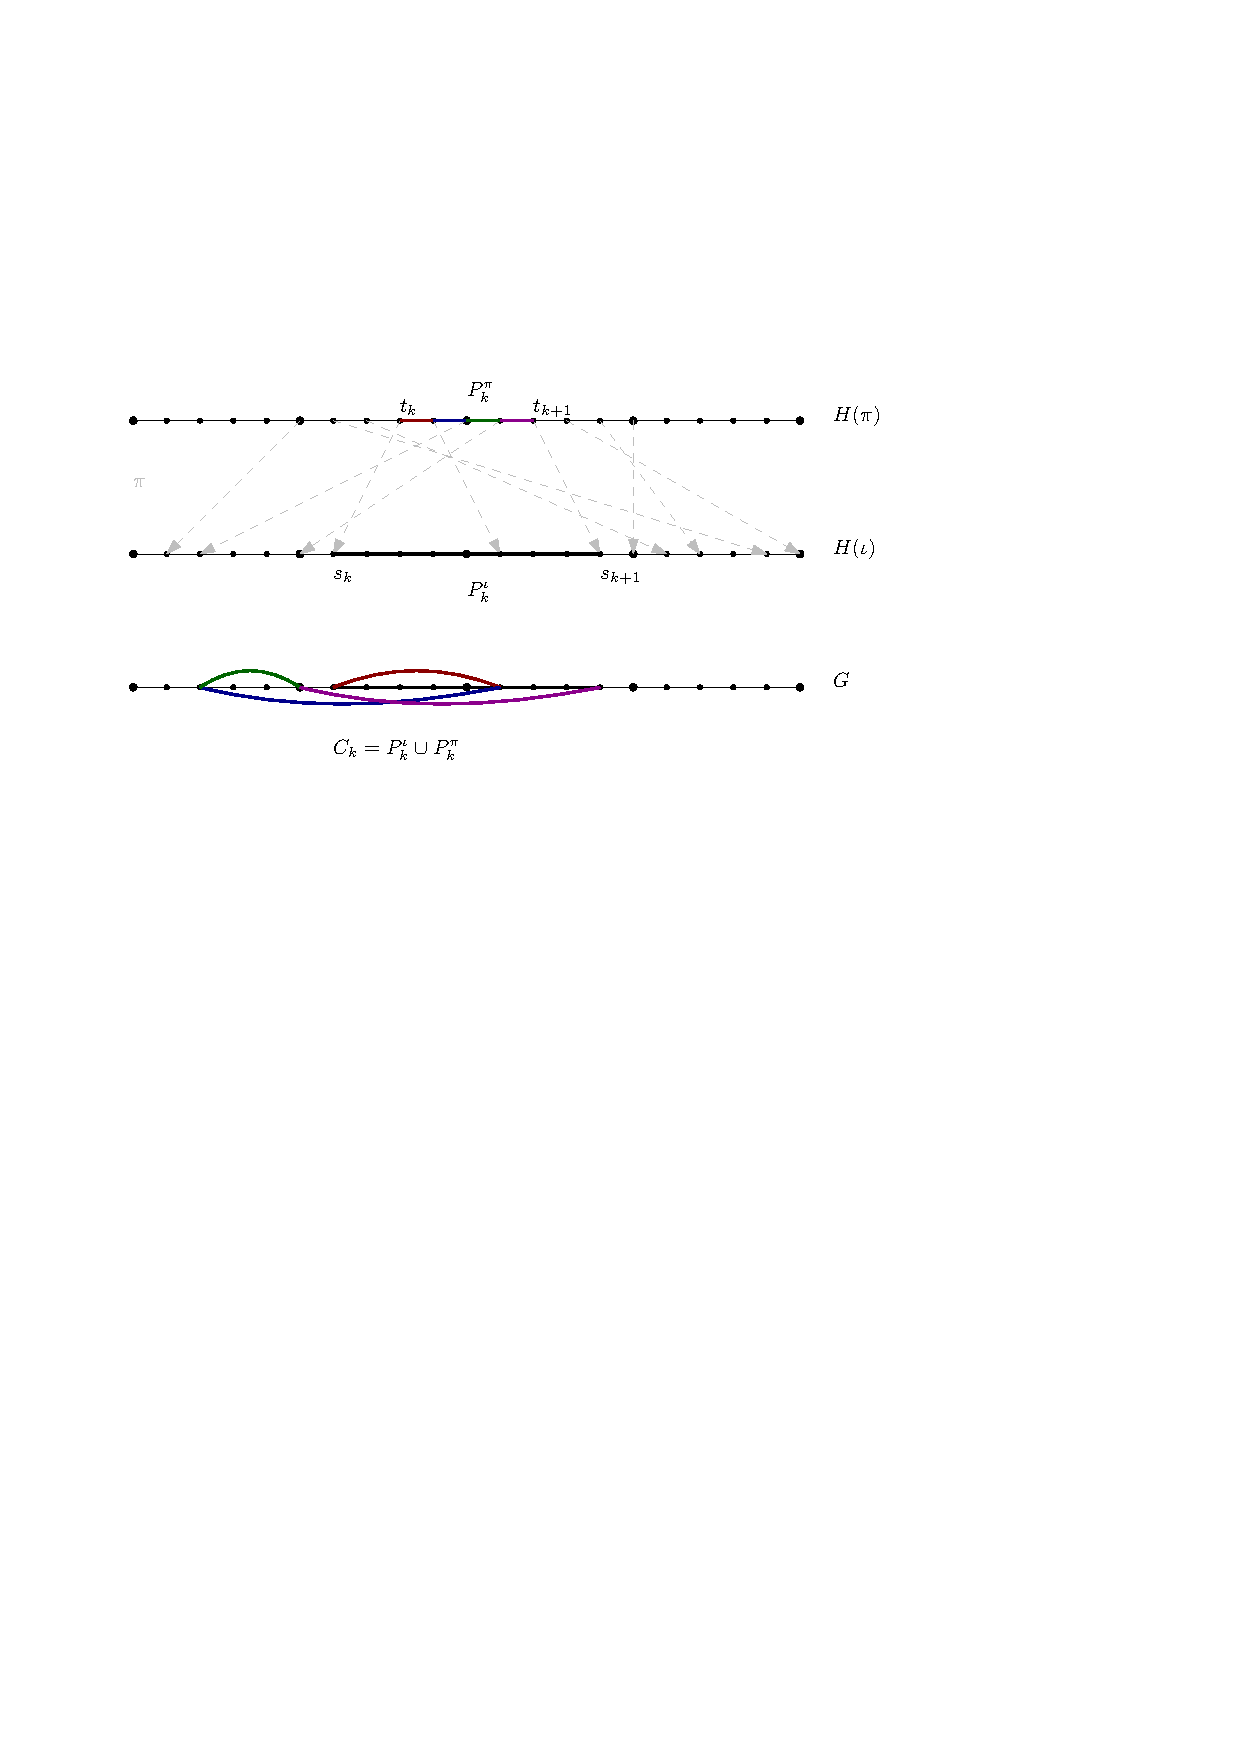
\includegraphics{../assets/742/cycledecomposition}
  \caption{One block of the decomposition of a random regular graph
    into short cycles. We obtain $C_k$ by identifying the vertices of
    $H(\iota)$ with the vertices of $H(\pi)$ according to $\pi$. }
  \label{fig:cycles}
\end{figure}

Let $m$ be a parameter depending on $n$; in this section, we choose $m = \sqrt{n\log n}$, while in the next section, we choose $m = C\sqrt{n}$. For simplicity, we assume that $m$ and $n/m$ are both integers. We partition $[n]$ into $n/m$ blocks $I_1,\ldots,I_{n/m}$ of size $m$: $I_k = \{(k-1)m+1,\ldots,(k-1)m+m\}$. Let $B_k$ be the event that $\pi(I_k) \cap I_k = \emptyset$. We think of $B_k$ as a bad event, and our goal in this section is to show that asymptotically almost surely, none of the $B_k$ happen. In order to show this, we estimate the probability that $B_k$ happens.

\begin{lemma} \label{lem:b-prob}
 For $k \in [n/m]$, $\prob{B_k} \leq \eee^{-m^2/n}$.
\end{lemma}
\begin{proof}
 Using $1-x \leq \eee^{-x}$, we calculate
\begin{equation}
 \prob{B_k} = \prod_{i=0}^{m-1} \left(1 - \frac{m}{n-i}\right) \leq \left(1 - \frac{m}{n}\right)^m \leq \eee^{-m^2/n} \eqperiod \qedhere
\end{equation}
\end{proof}

If $\overline{B_k}$ holds, we define $t_k$ to be the first point in $I_k$ such that $\pi(t_k) \in I_k$, and let $s_k = \pi(t_k)$.

\begin{lemma} \label{lem:cycle}
 Suppose $\overline{B_k}$ and $\overline{B_{k+1}}$ both hold (indices taken modulo $n/m$). Define a (possibly self-intersecting) cycle $C_k$ by taking two paths $P_k^\iota,P_k^\pi$ from $s_k = \pi(t_k)$ to $s_{k+1} = \pi(t_{k+1})$, one from each of the two Hamilton cycles:
\begin{align*}
 P_k^\iota &= (s_k,s_k+1),(s_k+1,s_k+2),\ldots,(s_{k+1}-1,s_{k+1}) \eqcomma \\
 P_k^\pi &= (\pi(t_k),\pi(t_k+1)),(\pi(t_k+1),\pi(t_k+2)),\ldots,(\pi(t_{k+1}-1),\pi(t_{k+1})) \eqperiod
\end{align*}
 The length of $C_k$ is at most $4m$.
\end{lemma}
\begin{proof}
 Assume for simplicity that $k \neq n/m$. Then $s_k,t_k \geq (k-1)m + 1$ and $s_{k+1},t_{k+1} \leq km + m$. The length of $C_k$ is $(s_{k+1} - s_k) + (t_{k+1} - t_k) \leq 4m-2$.
\end{proof}

If none of the bad events happen, then the cycles $C_1,\ldots,C_{n/m}$ cover all of the graph: by construction $\set{P_k^\iota}_k$ partitions $H(\iota)$, while $\set{P_k^\pi}_k$ partitions $H(\pi)$. Choosing $m$ accordingly, we can ensure that this happens asymptotically almost surely.

\begin{lemma} \label{lem:partition}
 Let $m = \sqrt{n\log n}$. Asymptotically almost surely, a graph chosen according to $\psHam(\iota) + \psHam(\pi)$ decomposes into $n/m$ cycles of %
 length at most $4m$.
\end{lemma}
\begin{proof}
 According to \expref{Lemma}{lem:b-prob}, for each $k \in [n/m]$, $\prob{B_k} \leq \eee^{-\log n} = 1/n$. A union bound shows that asymptotically almost surely, none of the $B_k$ happen. \expref{Lemma}{lem:cycle} shows that the graph decomposes into $n/m$ cycles of %
 length at most $4m$.
\end{proof}

The lemma easily implies the lower bound.

\begin{theorem} \label{thm:simple}
 Asymptotically almost surely, the space required to refute in PCR any Tseitin formula on a random $4$-regular graph on $n$ vertices is $\Bigomega{\sqrt{n/\log n}}$.
\end{theorem}
\begin{proof}
 By a symmetry argument, \expref{Lemma}{lem:partition} implies that asymptotically almost surely, a graph chosen according to $\psHam + \psHam$ decomposes into cycles of %
 length at most $4\sqrt{n \log n}$. \expref{Corollary}{cor:splitting} shows that asymptotically almost surely, the connectivity expansion of the graph is at least $\bigomega{n}$. \expref{Corollary}{cor:connected} shows that asymptotically almost surely, the graph is connected, and so the Tseitin formula is \Gnonsplittingnot. Hence \expref{Theorem}{th:tseitin-small-cycles-space-lower-bound} gives a lower bound of $\Omega(\sqrt{n/\log n})$.
\end{proof}

\subsection{Improved lower bound} \label{sec:improved}

In this section we improve the results of \expref{Section}{sec:simple} by showing that refuting a \Gnonsplitting Tseitin formula on a random $4$-regular graph on $n$ vertices requires space $\Bigomega{\sqrt{n}}$, asymptotically almost surely over the choice of the graph.

We use the general method of \expref{Section}{sec:simple}, with a different choice of $m$, namely $m = C\sqrt{n}$ for some constant $C$ to be determined later. Thinking of $B_k$ as an indicator variable, let $B = \sum_{k=1}^{n/m} B_k$. \expref{Lemma}{lem:b-prob} shows that $\expectation{B} \leq \eee^{-C^2} (n/m)$. We will show that asymptotically almost surely, $B \leq 2\eee^{-C^2} (n/m)$. This implies that the cycles $C_k$ together cover most of the graph, and therefore \expref{Corollary}{cor:tseitin-small-cycles-space-lower-bound} applies. The difficult part of the proof is showing that $B$ is concentrated around its mean.

Let $p = \prob{B_k}$ (all the probabilities are the same). We need the following strengthening of \expref{Lemma}{lem:b-prob}.

\begin{lemma} \label{lem:b-prob-limit}
 Let $p = \prob{B_k}$, where $B_k$ is the event that $I_k \cap \pi(I_k) = \emptyset$. As $n \tends \infty$, we have that $p \tends \eee^{-C^2}$.
\end{lemma}

In order to show that $B$ is concentrated around its mean, we show that for $k \neq l$, the events $B_k$ and $B_l$ are asymptotically negatively correlated.

\begin{lemma} \label{lem:correlation}
 For every $k \neq l \in [n/m]$, $\prob{B_k \land B_l} \leq p^2 + \littleoh{1}$.
\end{lemma}

We prove both lemmas below, but first, let us see how they imply the desired result. The idea is that since any two bad events are asymptotically negatively correlated, the variance of $B$ is small, and so Chebyshev's inequality shows that $B$ is concentrated around its mean.

\begin{lemma} \label{lem:concentration}
 Asymptotically almost surely, $B \leq 2\eee^{-C^2} (n/m)$.
\end{lemma}
\begin{proof}
 We have $\expectation{B} = (n/m)p$ and
\begin{align*}
 \variance{B} &= \expectation{B^2} - (\expectation{B})^2 \\ &=
 (n/m)p + (n/m)(n/m-1)(p^2 + \littleoh{1}) - (n/m)^2p^2 \\ &=
 (n/m)p(1-p) + \Littleoh{(n/m)^2} \eqcomma
\end{align*}
 using \expref{Lemma}{lem:correlation}. Chebyshev's inequality shows that
\begin{equation}
 \prob{|B-\expectation{B}|>\expectation{B}} \leq \frac{\variance{B}}{\expectation{B}^2} \leq \frac{(n/m)p + \Littleoh{(n/m)^2}}{(n/m)^2p^2} = \littleoh{1} \eqcomma
\end{equation}
 since $p = \bigomega{1}$ by \expref{Lemma}{lem:b-prob-limit}.
 Therefore asymptotically almost surely, $B \leq 2\expectation{B} = 2(n/m)p \leq 2\eee^{-C^2} (n/m)$, using \expref{Lemma}{lem:b-prob}.
\end{proof}

The preceding lemma shows that the fraction of bad indices (indices $k$ such that $B_k$ holds) is small. Say that a block $I_k$ is \emph{good} if $\overline{B_k}$ and $\overline{B_{k+1}}$ both hold, and say that it is \emph{supergood} if both $I_{k-1}$ and $I_k$ are good. \expref{Lemma}{lem:cycle} associates a cycle $C_k$ with each good block $I_k$. If $I_k$ is supergood, then the cycles $C_{k-1}$ and $C_k$ together cover the entire stretch of $I_k$, as the following lemma shows.

\begin{lemma} \label{lem:supergood}
 Suppose that block $I_k$ is supergood. Then the union of the cycles $C_{k-1},C_k$ given by \expref{Lemma}{lem:cycle} contains the path of length $m$ from $\min I_k$ to $\min I_{k+1}$ in $H(\iota)$, as well as the path of length $m$ from $\pi(\min I_k)$ to $\pi(\min I_{k+1})$ in $H(\pi)$.
\end{lemma}
\begin{proof}
 The cycle $C_{k-1}$ contains the path from $s_{k-1} < \min I_k$ to $s_k$ in $H(\iota)$. The cycle $C_k$ contains the path from $s_k$ to $s_{k+1} \geq \min I_{k+1}$ in $H(\iota)$. Both paths together cover the path from $\min I_k$ to $\min I_{k+1}$ in $H(\iota)$. The argument for $H(\pi)$ is identical.
\end{proof}

We can now prove an analogue of \expref{Lemma}{lem:partition}.

\begin{lemma} \label{lem:almost-partition}
 Let $m = C\sqrt{n}$. Asymptotically almost surely, a graph chosen according to $\psHam(\iota) + \psHam(\pi)$ decomposes into cycles of %
 length at most $4m$ and $t$ additional edges, where $t \leq 8\eee^{-C^2}n$.
\end{lemma}
\begin{proof}
 \expref{Lemma}{lem:concentration} shows that asymptotically almost surely, all but $4\eee^{-C^2} (n/m)$ of the $n/m$ blocks $I_1,\ldots,I_{n/m}$ are supergood, as each bad block prevents two blocks from being supergood. Let $\mathcal{C}$ be the (disjoint) union of all cycles $C_k$ constructed using \expref{Lemma}{lem:cycle} for all supergood blocks $I_k$. The lemma shows that each cycle has %
 length at most $4m$. \expref{Lemma}{lem:supergood} shows that $\mathcal{C}$ contains all but at most $8\eee^{-C^2} n$ edges of the graph.
\end{proof}

Replacing \expref{Theorem}{th:tseitin-small-cycles-space-lower-bound} with its corollary, \expref{Lemma}{lem:almost-partition} easily implies the lower bound.

\begin{theorem} \label{thm:improved}
 Asymptotically almost surely, the space required to refute in PCR any Tseitin formula on a random $4$-regular graph on $n$ vertices is $\Bigomega{\sqrt{n}}$.
\end{theorem}
\begin{proof}
  \expref{Corollary}{cor:splitting} shows that asymptotically almost surely, the connectivity expansion of the graph is at least $c_2 n$ %
  for some constant $c_2$. %
  %
  \expref{Lemma}{lem:almost-partition} implies that asymptotically almost surely, a graph chosen according to $\psHam + \psHam$ decomposes into cycles of %
 length at most $4C\sqrt{n}$ and $t$ additional edges, where $t \leq 8\eee^{-C^2}n$. For an appropriate choice of $C$ we have $t \leq (c_2/2)n$.
 \expref{Corollary}{cor:connected} shows that asymptotically almost surely, the graph is connected, and so the Tseitin formula is \Gnonsplittingnot.
 Hence \expref{Corollary}{cor:tseitin-small-cycles-space-lower-bound} gives a lower bound of $\Bigomega{\sqrt{n}}$.
\end{proof}

\subsubsection{Technical lemmas}

We now turn to the proofs of \expref{Lemma}{lem:b-prob-limit} and \expref{Lemma}{lem:correlation}. We start with the former.

\begin{proof}[Proof of \expref{Lemma}{lem:b-prob-limit}]
 It is easy to check that for $0 \leq x \leq 1/2$, $1-x \geq \eee^{-x-x^2}$. Therefore for large enough $n$,
\begin{equation}
 p = \prod_{i=0}^{m-1} \left(1 - \frac{m}{n-i}\right) \geq
 \left(1 - \frac{m}{n-m}\right)^m \geq
 \exp \left[ -\frac{m^2}{n-m}-\frac{m^3}{(n-m)^2} \right] \eqperiod
\end{equation}
 For large enough $n$, $m \leq n/2$, and so $m^2/(n-m) = m^2/n + m^3/(n(n-m)) \leq m^2/n + 2m^3/n^2$. Similarly, $m^3/(n-m)^2 \leq 4m^3/n^2$. Therefore, using $\eee^{-x} \geq 1-x$,
\begin{equation}
 p \geq \exp \left[ -\frac{m^2}{n} - 6\frac{m^3}{n^2} \right] = \exp \left[ -C^2 -\frac{6C^3}{\sqrt{n}} \right] \geq \eee^{-C^2} \left(1 - \frac{6C^3}{\sqrt{n}}\right) \eqperiod
\end{equation}
 Hence $\liminf p \geq \eee^{-C^2}$. \expref{Lemma}{lem:b-prob} shows that also $\limsup p \leq \eee^{-C^2}$.
\end{proof}

The proof of \expref{Lemma}{lem:correlation} is more involved. Recall that the lemma claims that the events $B_k$ and $B_l$ are asymptotically negatively correlated. In fact, they are asymptotically uncorrelated. Recall that $\prob{B_k}$ is roughly equal to $\eee^{-C^2}$. Given the value of $\pi$ on $I_k$, the probability $\prob{B_l}$ depends on $|\pi(I_k) \cap I_l|$. Typically, this intersection will be very small, and so $\prob{B_l}$ is also roughly equal to $\eee^{-C^2}$.

%
%
%

We will show that $|\pi(I_k) \cap I_l|$ is typically small using an
  extension of the well-known Chernoff bound due to Kabanets and
  Impagliazzo~\cite[Theorem 1.1]{KI}, attributed there to Panconesi and
  Srinivasan~\cite{PS}.


\begin{theorem} \label{thm:chernoff}
 Let $X_1,\ldots,X_r$ be Boolean random variables such that for any set $S \subseteq [r]$, $\prob{\bigwedge_{i \in S} X_i} \leq \delta^{|S|}$. Then for $\gamma \geq \delta$,
\begin{equation*}
 \PROB{\sum_{i=1}^r X_i \geq \gamma r} \leq \eee^{-2r(\gamma - \delta)^2} \eqperiod
\end{equation*}
\end{theorem}

%

The following lemma applies this bound to our situation (in an abstracted version).

\begin{lemma} \label{lem:prob-est}
 Let $a,b,c$ be integers such that $a \geq b,c$, and let $T$ be a random subset of $[a]$ of size $b$. For all $\rho \geq 1$,
 \begin{equation*}
  \prob{|T \cap [c]| \geq \rho (bc/a)} \leq \eee^{-2c(\rho-1)^2(b/a)^2} \eqperiod
 \end{equation*}
\end{lemma}
\begin{proof}
 For $i \in [c]$, let $X_i$ be the event that $i \in T$. For $S \subseteq [c]$ such that $|S| \leq b$,
\begin{equation}
 \prob[T]{S \subseteq T} = \frac{\binom{a-|S|}{b-|S|}}{\binom{a}{b}} =
 \prod_{k=0}^{|S|-1} \frac{b-k}{a-k} \leq \left(\frac{b}{a}\right)^{|S|} \eqperiod
\end{equation}
 Therefore we can apply \expref{Theorem}{thm:chernoff} with $r = c$, $\delta = b/a$ and $\gamma = \rho(b/a)$.
\end{proof}

We can now prove \expref{Lemma}{lem:correlation}.

\begin{proof}[Proof of \expref{Lemma}{lem:correlation}]
 We will show that $\condprob{B_l}{B_k} \leq p + \littleoh{1}$. This implies that $\prob{B_k \land B_l} = \prob{B_k} \condprob{B_l}{B_k} \leq p(p + \littleoh{1}) = p^2 + \littleoh{1}$.

 Assuming the event $B_k$ happens, $\pi(I_k)$ is a random subset of $[n] \setminus I_k$ of size $m$. Plugging $a = n-m$ and $b = c = m$ in \expref{Lemma}{lem:prob-est}, we deduce that for all $\rho \geq 1$ and large enough $n$
 %
 \begin{align}
  \condprob{|\pi(I_k) \cap I_l| \geq \rho C^2}{B_k} &\leq \eee^{-2(\rho-1)^2m(m/(n-m))^2} \\&\leq \eee^{-2(\rho-1)^2 m^3/n^2} = \eee^{-2C^3(\rho-1)^2/\sqrt{n}} \eqperiod
 \end{align}
 Hence with probability $1-\littleoh{1}$ given $B_k$, $D \eqdef |\pi(I_k) \cap I_l| \leq \sqrt{m\log m}$. Now
\begin{equation}
 \condprob{B_l}{D=d} = \prod_{i=0}^{m-1} \left(1 - \frac{m-d}{n-m-i}\right) \leq \left(1 - \frac{m-d}{n}\right)^m \leq \eee^{-m(m-d)/n} \eqperiod
\end{equation}
%
%
 For $0 \leq x \leq 1$, one can check that $\eee^x \leq 1 + 2x$. Hence
\begin{align}
 \condprob{B_l}{D \leq \sqrt{m\log m}} &\leq \eee^{-m(m-\sqrt{m\log m})/n} \\ &= \eee^{-C^2+m\sqrt{m\log m}/n} \leq \eee^{-C^2} \left(1 + \frac{2m\sqrt{m\log m}}{n}\right) \eqperiod
\end{align}
 Using \expref{Lemma}{lem:b-prob-limit}, we deduce that $\condprob{B_l}{D \leq \sqrt{m\log m}} \leq \eee^{-C^2} + \littleoh{1} = p + \littleoh{1}$.
 We conclude that $\condprob{B_l}{B_k} = p + \littleoh{1}$ and so $\prob{B_k \land B_l} = p^2 + \littleoh{1}$.
\end{proof}

%

\subsection{Regular graphs of degree larger than four}
Wormald~\cite[Corollary 4.17]{W} showed that when $d > 4$, a random $d$-regular graph can be obtained (up to contiguity) by taking the disjoint union of a random $4$-regular graph and a random $(d-4)$-regular graph, a result summarized in the following theorem (see also~\cite[Corollary 9.44]{JLR}).

\begin{theorem}\label{th:regular}
 For $d > 4$ we have $\psReg_d \approx \psReg_4 \oplus \psReg_{d-4}$. Furthermore, the probability that a uniformly random $4$-regular graph and a uniformly random $(d-4)$-regular graph do not intersect tends to a positive constant.
\end{theorem}

A Tseitin formula on a random $d$-regular graph generated according to $\psReg_4 \oplus \psReg_{d-4}$ is harder to refute than a Tseitin formula on a random $4$-regular graph, and so we can generalize \refth{thm:improved} to random $d$-regular graphs for arbitrary $d \geq 4$.

\begin{theorem}[restatement of \refth{thm:improved-general}]
 Let $d \geq 4$. Asymptotically almost surely, the space required to refute in PCR any Tseitin formula on a random $d$-regular graph on $n$ vertices is $\Bigomega{\sqrt{n}}$.
\end{theorem}
\begin{proof}
 If $d = 4$ then \refth{thm:improved} already applies, so assume $d > 4$.
 Let $G_1$ be a random $4$-regular graph, and let $G_2$ be a random $(d-4)$-regular graph. The graph $G = G_1 + G_2$ is distributed according to $\psReg_4 + \psReg_{d-4}$. We show below that asymptotically almost surely, the space required to refute in PCR any Tseitin formula on $G$ is $\Bigomega{\sqrt{n}}$. Since $G_1$ and $G_2$ are disjoint with constant probability according to \refth{th:regular}, the theorem follows.

 Let $\alpha$ be an arbitrary assignment to the edges of $G_2$. \refobsP{obs:induced-graph-and-assignments} shows that for every function $f$, $\restrict{\tseitinnot{G}{\tseitincharge}}{\alpha} = \tseitinnot{G_1}{\gamma}$ for some other function $\gamma$. By a restriction argument, any PCR refutation of $\tseitinnot{G}{\tseitincharge}$ in space $S$ can be translated to a PCR refutation of $\tseitinnot{G_1}{\gamma}$ in space at most $S$. \refthP{thm:improved} shows that asymptotically almost surely, we must have $S  = \Bigomega{\sqrt{n}}$.
\end{proof}


\section{Bonacina--Galesi framework and the Functional Pigeonhole Principle}
\label{sec:limitations}

  We now discuss the intrinsic limitations of the techniques employed
  so far. In \expref{Section}{sec:fphp-no-kextendible} we show that
  Bonacina--Galesi framework does not allow to prove PCR space lower
  bounds for an interesting formula like functional pigeonhole
  principle. In \expref{Section}{sec:varweightconstrained} we show that
  restricting to PC does not make the problem easier.

\subsection{FPHP formulas do not have \KextendibleNok families}
\label{sec:fphp-no-kextendible}

One of the limits of the Bonacina--Galesi framework is that we cannot
apply it to formulas for which fixing a small set of variables causes
a lot of unit clause propagation. Indeed, most of the lower bound
strategies in this paper aim to control this phenomenon (see for
example \reflem{lem:substitution}). For the functional pigeonhole
principle these strategies do not work, as we now prove.


\begin{definition}\label{def:fphpformula}
  The \introduceterm{functional pigeonhole principle} on $m$ pigeons and $n$ holes is the formula defined on variables $x_{ij}$ for $i\in[m]$ and $j\in[n]$, made of the following clauses:
  \begin{align}
    \Lor_{j\in[n]} x_{ij} && \text{for all $i\in[m]$;} \tag{pigeon axioms}\\
    \lnot{x_{ij}} \lor \lnot{x_{i'j}} && \text{for any
      $i\not=i'\in[m]$ and $j\in[n]$;} \tag{hole axioms}\\
    \lnot{x_{ij}} \lor \lnot{x_{ij'}} && \text{for any $i\in[m]$ and
      $j\not=j'\in[n]$.\tag{functional axioms}}
  \end{align}
\end{definition}

%

%
%
%
%
%

It is already known that this formula requires large space in
resolution~\cite{BW01ShortProofs,AD08CombinatoricalCharacterization}.
%
Thanks to~\cite{GKT19SpaceWidth} we know that this formula needs
$\Omega(\sqrt{n})$ monomial space as well.
%
We suspect that the true lower bound is actually $\Omega(n)$, however
the Bonacina--Galesi framework is not strong enough to prove it.
That framework cannot even prove a non constant lower bound for
functional pigeonhole principle.

\begin{theorem}[restatement of \expref{Theorem}{th:no-kextendible}]
  There is no \kextendible family for $\fphpnot{m}{n}$ for $\kextendiblenot > 1$.
\end{theorem}
\begin{proof}

  Assume that there is \akextendible family $\kextendfamily$ for
  the formula $\fphpnot{m}{n}$ which respects some satisfiable
  $F'\subseteq \fphpnot{m}{n}$, for $\kextendiblenot>1$.

  Let $C$ be any clause in $\fphpnot{m}{n}\setminus F'$; such clause exists because $\fphpnot{m}{n}$ is a contradiction.
  %
  The \extensionproperty of \kextendfamily implies that there is a
  pair $(\{Q_{1}\}, H_{1} )\in\kextendfamily$, where $H_{1}$ satisfies $C$.

  Recall that $0$ encodes true, and $1$ encodes false. Pick a
  variable $x_{ij}$ in $Q_{1}$. In $H_{1}$ there is at least one
  partial assignment for which $x_{ij}=0$, and for any such assignment
  it holds that $x_{i'j}=1$ and $x_{ij'}=1$ for all $i'\not=i$ and
  $j'\not=j$, otherwise an initial clause would be false.

  Indeed, fix $v$ to be any of these variables (either $x_{i'j}$ or
  $x_{ij'}$); the clause $\lnot{x_{ij}} \lor \lnot{v}$ is an axiom.
  %
  If $v \not\in Q_{1}$ then this clause is not in $F'$ because of the
  \respectfulness of \kextendfamily, and furthermore there is at
  least one assignment in $H_{1}$ which does not satisfy it (\ieComma any assignment with
  $x_{ij}=0$).
  %
  The \extensionproperty of \kextendfamily guarantees that there is
  $(\{Q_{1},Q_{2}\},H_{1}\times H_{2}) \in \kextendfamily$ with $v\in
  Q_{2}$, such that $H_{1}\times H_{2}$ satisfies $\lnot{x_{ij}} \lor
  \lnot{v}$. But this contradicts the fact that $H_{1}\times H_{2}$
  contains the assignment $\{x_{ij}=1,v=1\}$, which falsifies
  $\lnot{x_{ij}} \lor \lnot{v}$.


  It follows that $\setdescr{x_{i'j},x_{ij'}}{i'\not=i \text{\ and\
    } j'\not=j} \subseteq Q_{1}$, and that $H_{1}$ satisfies all
  axioms involving either pigeon $i$ or hole $j$.
  %
  We have just shown that assuming some $x_{ij}\in Q_{1}$, we get
  \mbox{$\setdescr{x_{i'j},x_{ij'}}{i'\in[m], j'\in[n]}\subseteq
    Q_{1}$}. This choice was arbitrary, so it follows that for any
  $i\in[m], j\in[n]$, the variable $x_{ij}$ is in $Q_{1}$. In other
  words, $Q_1$ contains all the variables. Since
  $\fphpnot{m}{n}\setminus F'$ is contradictory, every assignment in
  $H_1$ falsifies some clause, and so the \extensionproperty fails for
  any such clause.  We conclude that $\fphpnot{m}{n}$ has no
  $2$-extendible family.
  \end{proof}

 %
\subsection{Formulas with equal PC and PCR space complexities}
\label{sec:varweightconstrained}


Although finding an \kextendible{} family for the functional
pigeonhole principle (and hence proving a linear space lower bound) is not
feasible, we might try and prove a weaker PC space lower
bound. However, as we have pointed out in
\refsec{sec:space-compl-funct}, in the case of functional pigeonhole
principle this makes no difference. In this section, we prove formally
this result for a broader class of formulas that is captured by the
following definition.

\begin{definition}\label{def:var-weight-constrained}
  We say that a CNF formula~$F$ is
  \introduceterm{\varweightconstrained{}} if for every variable $x$
  appearing in $F$ there exists a clause $C_x \in F$ with the
  following properties:
  \begin{enumerate}
  \item All literals in $C_x$ are positive;
  \item $x$ is one of the variables appearing in $C_x$;
  \item For every two distinct variables $y, z$ appearing in $C_x$,
    clause $\olnot{y} \lor \olnot{z}$ is in $F$.
  \end{enumerate}
  For each variable $x$ we refer to $C_x$ as the
  \introduceterm{\varneighborhoodclause{x}}.
\end{definition}

In such formulas each negative literal can be replaced with a
clause/monomial consisting of only positive literals that has the same
semantic meaning. Thus, we can turn a PCR refutation into a PC
refutation without any substantial loss of space. In order for us to
be able to show that such a refutation is a valid PC refutation we
need to show that there are PC derivations of these monomials that use
small space.

\begin{theorem}\label{th:varweightconstrained}
  For a \varweightconstrained{} CNF formula~$F$, where each clause has
  a constant number of negative literals, it holds that
  $\mspaceref[PC]{F} = \bigtheta{\mspaceref[PCR]{F}}$.
\end{theorem}

%

\begin{proof}
  We can easily see that PCR simulates PC with only a constant loss in
  space. The only problem in the simulation could arise when
  downloading an axiom that has negative literals. Nevertheless, it is
  not hard to prove that PCR can expand every axiom to its PC form
  while respecting the stated space bound.

  In the other direction, we prove that PC can simulate a PCR
  refutation of $F$. Let $\pi$ be a PCR refutation of $F$ in space at
  most $s$. As $F$ is a \varweightconstrained{} formula, for every
  variable $x$ we can fix its \varneighborhoodclause{x} $C_x$. Let us
  denote by $\varneighbors{x}$ the set of variables from $C_x$
  excluding~$x$. We transform the PCR refutation $\pi$ into a PC
  refutation by replacing each negative literal $\olnot{x}$ with the
  monomial $\prod_{y \in \varneighbors{x}} y$. Obviously this
  transformation preserves space and we need to show that the
  transformed configurations form a backbone of a valid PC refutation.

  If the PCR refutation deletes a polynomial, we delete the
  appropriate transformed polynomial from the configuration in the
  PC refutation. Similarly, in the case of linear combination steps we
  just deduce the linear combination of the transformed
  polynomials. Hence, these two types of steps can be done without any
  loss in space. In the case of multiplication with a literal, if the
  literal is positive we multiply the appropriate transformed
  polynomial with the same literal. Otherwise, the literal is negative
  and we multiply the polynomial with all the variables in
  $\varneighbors{x}$, where $\olnot{x}$ is the literal, while making
  sure to delete the intermediate polynomials when they are no longer
  needed. In this way we derive the transformed polynomial in at most
  $\bigoh{s}$ space.

  The axiom download steps are the only ones that remain. In the case
  of Boolean axiom download, if we downloaded an axiom for a positive
  literal, we just download the appropriate axiom in the PC
  refutation. Otherwise, the Boolean axiom corresponds to some
  negative literal $\olnot{x}$ and we need to derive the polynomial
  $\prod_{y \in \varneighbors{x}} y^2 - \prod_{y \in \varneighbors{x}}
  y$. This is done by downloading the Boolean axioms for each~$y \in
  \varneighbors{x}$ and combining them to get the transformed
  polynomial. Let $\booleanaxiompartial^2 - \booleanaxiompartial$ be
  one of the intermediate polynomials in the derivation of the
  transformed Boolean axiom, where $\booleanaxiompartial$ is a
  monomial formed by multiplying the variables in some subset of
  $\varneighbors{x}$. Then, for some variable $y$ not mentioned in
  $\booleanaxiompartial$, we derive $(\booleanaxiompartial y)^2 -
  \booleanaxiompartial y$ by downloading $y^2 - y$ and taking the
  linear combination of $y(\booleanaxiompartial^2 -
  \booleanaxiompartial)$ and $\booleanaxiompartial^2(y^2 - y)$. This
  PC derivation uses $\bigoh{1}$ more monomials than the PCR axiom
  download.

  When the PCR proof downloads the complementarity axiom $1 - x -
  \olnot{x}$, the corresponding PC proof needs to derive the
  polynomial $1 - x - \prod_{y \in \varneighbors{x}} y$. Let
  $\varneighbors{x} = \set{y_1, \ldots, y_l}$. We derive the
  transformed polynomial by successively deriving polynomials
  \begin{equation}
    \complementarityiter{i} = \prod_{k = i + 1}^l y_k - x \prod_{k = i + 1}^l y_k - \prod_k y_k \eqcomma
  \end{equation}
  for $i = 1, \ldots, l$. Note that $\complementarityiter{l}$ is our
  transformed polynomial. The first $\complementarityiter{1}$ in the
  PC proof can be derived by downloading the axiom $(1 - x)(1 - y_1)$
  and multiplying it with variables $y_2, \ldots, y_l$ in order to get
  %
  %
  $\complementarityiter{1} + x \prod_k y_k$. Subtracting from it
  the~\varneighborhoodclause{x} $C_x = x \prod_k y_k$ we get
  $\complementarityiter{1}$.

  %
  %

  We proceed to derive $\complementarityiter{i + 1}$ from
  $\complementarityiter{i}$ for all~$i$. Similarly as before, we start
  by downloading the axiom~$(1 - x)(1 - y_{i + 1})$ and multiplying it
  with variables $y_{i + 2}, \ldots, y_l$ in order to get
  %
  %
  $\complementarityiter{i + 1} - \complementarityiter{i}$. Adding this
  polynomial to~$\complementarityiter{i}$ we derive the $(i + 1)$st
  polynomial~$\complementarityiter{i + 1}$ in our derivation of the
  transformed complementarity axiom. This PC derivation uses
  $\bigoh{1}$ more monomials than the PCR proof and all axioms of the
  form~$(1 - x)(1 - y_i)$ exist because $F$ is
  \varweightconstrained{}.

  In the case of axiom download step for a clause axiom, we again have
  two cases. If all literals of the axiom are positive we download the
  corresponding axiom in the PC proof. Otherwise, we can write the
  axiom as $\olnot{x_1} \cdots \olnot{x_s} \cdot x_{s + 1} \cdots
  x_l$, where $s$ is the number of its negative literals.
  Let us denote by $\negativeaxiomiter{i}$
  the polynomial
  \begin{equation}
    \negativeaxiomiter{i} = \prod_{y_1 \in \varneighbors{x_1}} y_1 \cdots \prod_{y_i \in
      \varneighbors{x_i}} y_i (1 - x_{i + 1}) \cdots (1 - x_s) x_{s + 1} \cdots x_l \eqcomma
  \end{equation}
  where $i$ ranges over $0, \ldots, s$. Note that
  $\negativeaxiomiter{0}$ is the original PC axiom, while
  $\negativeaxiomiter{s}$ is the transformed axiom that we want to
  derive. Also, let us denote by $\remainingpoly{i}$ the polynomial
  \begin{equation}
    \remainingpoly{i} = \prod_{y_1 \in \varneighbors{x_1}} y_1 \cdots \prod_{y_{i - 1} \in \varneighbors{x_{i - 1}}} y_{i - 1} \cdot (1 - x_{i + 1}) \cdots (1 - x_s) x_{s + 1} \cdots x_l \eqcomma
  \end{equation}
  for $i$ ranging from $1$ to $s$, that is $\negativeaxiomiter{i} =
  \remainingpoly{i} \prod_{y_i \in \varneighbors{x_i}} y_i =
  \remainingpoly{i + 1} (1 - x_{i + 1})$.

  We first derive $\negativeaxiomiter{1}$ by deriving the transformed
  complementarity axiom $1 - x_1 - \prod_{y_1 \in \varneighbors{x_1}}
  y_1$ for the variable $x_1$ and multiplying it with
  $\remainingpoly{1}$ in order to get
  %
  %
  $\negativeaxiomiter{0} - \negativeaxiomiter{1}$. Now we can get
  $\negativeaxiomiter{1}$ by subtracting the derived polynomial from
  the PC axiom $\negativeaxiomiter{0}$.

  %
  %
  %
  %

  We proceed to derive $\negativeaxiomiter{s}$ by deriving
  $\negativeaxiomiter{i + 1}$ from $\negativeaxiomiter{i}$ for all $i$
  from 1 to $s - 1$. This is again done by first deriving the
  appropriate complementarity axiom $1 - x_{i + 1} - \prod_{y_{i + 1}
    \in \varneighbors{x_{i + 1}}} y_{i + 1}$ and multiplying it by
  $\remainingpoly{i + 1}$ in order to get
  %
  %
  %
  $\negativeaxiomiter{i} - \negativeaxiomiter{i + 1}$. Subtracting the
  derived polynomial from previously derived~$\negativeaxiomiter{i}$,
  we get the $(i + 1)$st polynomial in our derivation. These steps use
  $\bigoh{2^{s}}$ monomials, which is constant by the theorem hypothesis,
  and the PC derivation of the transformed axiom uses at most
  $\bigoh{1}$ monomials more than the PCR axiom download step.

  Hence, the theorem follows. Also, although we have ignored the
  constants involved in the simulation, these constants can be
  computed explicitly and are small. The only possible exception is
  the additive constant $\bigoh{2^{s^{*}}}$, where $s^{*}$ is the
  largest number of negative literals in a clause of $F$.
\end{proof}

An obvious example of the \varweightconstrained{} formula is the
functional pigeonhole principle.

\begin{corollary}[restatement %
  of \refth{th:fphppcequalpcrspace}]\label{cor:fphppcequalpcrspace}
  It holds that
  \begin{equation*}
    \mspaceref[PCR]{\fphpnot{m}{n}} = \bigtheta{\mspaceref[PC]{\fphpnot{m}{n}}} \eqperiod
  \end{equation*}
\end{corollary}
\begin{proof}
  It is easy to see that $\fphpnot{m}{n}$ formula is
  \varweightconstrained{}, as every variable appears in some pigeon
  axiom that is constrained by the functional axioms. Also,
  $\fphpnot{m}{n}$ has at most $2$ negative literals in each clause
  and hence we have that $\mspaceref[PCR]{\fphpnot{m}{n}} =
  \bigtheta{\mspaceref[PC]{\fphpnot{m}{n}}}$.
\end{proof}

%
%
%
%
%
%
%

Actually, we can say even more about the space complexity of the
functional pigeonhole principle formulas. In \cite{FLNRT15SpaceCplx},
the authors prove that the PCR space complexity of $\fphpnot{m}{n}$ is
equal (up to constant factors) to the PCR space complexity of the
extended formula $\efphpnot{m}{n}$, where $\efphpnot{m}{n}$ is the
canonical equivalent $3$-CNF version%
%
\footnote{We substitute every clause $\lita_{1}\lor\lita_{2}\lor \ldots \lor
  \lita_{k}$, which has more than three literals, with the formula
$(\lita_{1}\lor y_{1}) \land
(\lnot{y_{1}}\lor\lita_{2}\lor y_{2})
\land \ldots \land
(\lnot{y_{i-1}}\lor\lita_{i}\lor y_{i})
\land \ldots \land
(\lnot{y_{k-1}}\lor\lita_{k}) $
%
where for each substituted clause all variables $y_{i}$ are new. The
substituted formula is a $3$-CNF and it is satisfiable if and only if
the original one is. It is also easy to deduce the original clause
from the substituting formula.}
%
of the formula $\fphpnot{m}{n}$. Hence, we have that the PC
space complexity lower bound for $\fphpnot{m}{n}$ would actually lower
bound the PCR space complexity of $\efphpnot{m}{n}$.

This holds in greater generality for \varweightconstrained{} formulas
that also fulfill the following technical condition: $F$ is a
\emph{weight-constrained} CNF formula if for each clause $\lita_{1} \lor
\lita_{2} \lor \ldots \lor \lita_{m}$ of $F$ with more than three literals,
the formula also contains clauses $\lnot{\lita_{i}} \lor \lnot{\lita_{j}}$ for
all $1 \leq i < j \leq m$.
%
We stress the fact that the conditions of being weight-constrained and \varweightconstrained{} are incomparable.

\begin{corollary}
  For a simultaneously weight-constrained and a
  \varweightconstrained{} formula~$F$, where each clause has a constant
  number of negative literals, it holds that
  \begin{equation*}
    \mspaceref[PCR]{\extendedversion{F}} = \bigtheta{\mspaceref[PCR]{F}} = \bigtheta{\mspaceref[PC]{F}} \eqperiod
  \end{equation*}
\end{corollary}
 
%

\section{Concluding remarks}
\label{sec:concluding-remarks}

In this paper, following up on 
%
work in
\cite{BNT13SomeTradeoffs,BG15Framework,FLNRT15SpaceCplx,HN12VirtueSuccinctProofs},
we report further progress on understanding space complexity in
polynomial calculus and how the space measure is related to size and degree.
Specifically, we separate size and degree from
space, and provide some circumstantial evidence for the conjecture
that degree might be a lower bound on space in 
%
polynomial calculus (PC) and polynomial calculus resolution (PCR),
where PCR is a strengthening of PC with separate formal dual variables
for negated literals (making PCR more suited to the
study of space complexity).
We also prove space lower bounds for a large class of Tseitin
formulas, a well-studied formula family for which nothing was
previously known regarding PCR space.

We 
%
believe that our lower bounds for Tseitin formulas
over random graphs are \emph{not} optimal, however. And for the
functional pigeonhole principle, we show that the technical tools
developed in~%
\cite{BG15Framework}
cannot prove any non-constant PCR space lower bounds. Although we have
not been able to prove this, we believe that similar impossibility
results should hold also for ordering principle formulas and for the
canonical \mbox{$3$-CNF} version of the pigeonhole principle.
Since all of these formulas require large degree in PCR
and large space in resolution, it is natural to suspect that
they should be hard for PCR space as well.
The fact that arguments along the lines of~%
\cite{BG15Framework}
do not seem to be able to establish this suggests that we are still
far from a combinatorial characterization of degree analogous to
the characterization of resolution width 
in~%
\cite{AD08CombinatoricalCharacterization}.

It thus remains a major open problem to understand the exact
relation between degree and space in PC/PCR.
Subsequent to the conference version of this
paper~\cite{conf-version}, %
Galesi \etal~\cite{GKT19SpaceWidth} have shown that
%
%
%
the square root of resolution width %
is a lower bound on PCR space %
(and hence so is the square root of polynomial calculus degree), %
but it is not clear whether this square root loss is necessary.
For formulas such as Tseitin formulas, functional PHP formulas, and
ordering principle formulas, it seems reasonable to believe that PCR space
lower bounds without the square root should hold.

Also, our separations of size and degree on the one hand and space on
the other depend on the characteristic of the 
underlying field, in that the characteristic must be chosen
first and the formula  family exhibiting the separation works only
for this specific characteristic.
It follows from~\cite{GKT19SpaceWidth} that there are formulas
(namely, graph-based versions of onto functional pigeonhole principle
formulas) of size $\bigtheta{n}$ that can be refuted in polynomial
calculus  in constant degree and size~$\bigoh{n \log n}$,
but that require PCR space~$\Bigomega{\sqrt{n}}$.
However, this is still weaker than our separation results, which
depend on the characteristic but gives an optimal separation with a
space lower bound~$\bigomega{n}$. The separation results
in~\cite{GKT19SpaceWidth} and our paper are therefore incomparable,
and it remains an interesting open problem to establish an optimal
separation that would also be independent of the characteristic of the
underlying field.

Finally, an intriguing question is how (monomial) space in PC/PCR is
related to (clause) space in resolution. Since there are separations
known for polynomial calculus size versus resolution length, and for
polynomial calculus degree versus resolution width, it would seem
reasonable to expect that PCR should be strictly stronger than
resolution also with respect to space, but this is completely open.%
\footnote{%
  For completeness, we mention that there is a very weak
  (constant-factor) separation in~\cite{ABRW02SpaceComplexity}, but it
  crucially depends on a somewhat artificial definition of space where
  monomials are \emph{not} counted with repetitions.}  
%
%
Turning this question around, one can also ask to
what extent space lower bound techniques for
resolution carry over to PC/PCR. Since so far we do not know of any
%
counterexamples, %
it is natural to wonder, for instance, whether
\introduceterm{semiwide} CNF formulas as defined in~%
\cite{ABRW02SpaceComplexity} have high space complexity not only in
resolution but also in PCR.
 
%
%

\appendix
%
\section{PCR space lower bounds from extendible families}
\label{sec:bg-framework}

%
%
%
%
%
For the sake of self-containment, in this appendix we give an
exposition of the Bonacina--Galesi
framework~\cite{BG15Framework} for proving space lower bounds
in Polynomial Calculus. %
That is, we
show how the existence of an
\kextendible family for a large value of $\kextendiblenot{}$
implies such bounds. %
Our proof follows the same high level structure as Bonacina and Galesi's, except that some of the technical definitions are more elementary. Furthermore, we observe that this
framework can actually prove space lower
bounds for a proof system that %
is   %
stronger than PC or PCR.

\begin{definition}[Functional Calculus (FC)]
  \label{def:fc}
A \introduceterm{functional calculus} configuration is a set of arbitrary Boolean functions over Boolean variables. There is a single derivation rule, \introduceterm{semantic implication}, where $g$ can be inferred from $f_1,\ldots,f_n$ if every assignment that satisfies $f_1\land\cdots\land f_n$ also satisfies $g$.
\end{definition}

Verifying a proof in FC is $\coNP$-complete, and so FC is not a proof system in the sense of Cook and Reckhow~\cite{CR79Relative} unless $\coNP = \NP$.

There are many different circuit representations of the same Boolean function, so we need to choose a minimal representation in order to define space.

\begin{definition}
  \label{def:fcspace}
  Let $\pcsp$ be a FC configuration. A %
  set~$U=\set{m_1,\ldots,m_s}$ of monomials
  \introduceterm{defines} $\pcsp$ if for every function $f\in\pcsp$ there is a function $g$ such that $g(m_1,\ldots,m_s)\equiv f(x_1,\ldots,x_n)$. The \introduceterm{monomial space} of $\pcsp$, denoted by $\mspaceof{\pcsp}$, is the minimum size of a %
  defining set of monomials.
\end{definition}

We can interpret polynomials in PCR as Boolean functions if we project them to the Boolean ring $\fieldstd[x,\olnot{x}, y, \olnot{y}, \ldots]/\Span{x^2-x,1-x-\olnot{x},\olnot{x}^2-\olnot{x},y^2-y,\ldots}$. Furthermore, the set of monomials in a PCR configuration counted without repetitions is a %
defining set of monomials
for a FC configuration. Therefore we can view every proof in PCR as a proof in FC that uses at most the same space. In particular, $\mspaceref[\fcnot]{F}\leq \mspaceref[\pcrnot]{F}$.

We now prove \refth{th:space-lower-bound}, following Bonacina and Galesi~\cite{BG15Framework}. The general plan of the proof is to consider a FC derivation from a formula $F$ in small space, and show that every configuration arising in the derivation is satisfiable. Since a refutation ends with an unsatisfiable configuration, the derivation is not a refutation.

In order to show that every configuration arising in the derivation is satisfiable, we maintain a satisfiability witness, in the form of a structured set of assignments together with a CNF formula.  The following definition captures the sense in which a satisfiability witness guarantees that a configuration is satisfiable. Fix a %
set~$V$ of variables
and consider partitions and total assignments with respect to this set.
Recall that a total assignment assigns a value to \emph{each} variable in $V$.

\begin{definition}
  \label{def:partialmodels}
  Let $\structuredassignmentsnot$ be a structured set of assignments, $G$ be a
  CNF formula, and $\pcsp$ be a set of Boolean functions.
  We write $G \partialmodels \pcsp$ if every total assignment that extends some partial assignment in $\assignmentsetnot$ and satisfies $G$ also satisfies $\pcsp$.
\end{definition}

In the proof, $\pcsp$ is one of the configurations that form the FC refutation, and $\structuredassignmentsnot,G$ together form a satisfiability witness for $\pcsp$. The CNF $G$ is composed of two parts: a satisfiable subset $F' \subset F$, which could be empty, and a 2-CNF $M$ with a very specific form given by the following definition.

\begin{definition}
  \label{def:transversal}
  Let $M$ be a 2-CNF formula over the variables $V$. We say that $M$ is a \introduceterm{transversal} of a partial partition $\partitionnot$ defined on $V$ if $M$ mentions exactly one variable from each block $Q_i \in \partitionnot$, and each mentioned variable appears exactly once. (In particular, $\setsize{\partitionnot}$ must be even and the number of clauses in $M$ is $\setsize{\partitionnot}/2$.)
\end{definition}

A transversal CNF formula is always satisfiable, and so for $F' = \emptyset$, any configuration $\pcsp$ that has a satisfiability witness of this form must in fact be satisfiable. To handle an arbitrary $F'$, we add the requirement that $\structuredassignmentsnot$ respect $F'$. Finally, we can formally define the concept of satisfiability witness.
%

\begin{definition}
 \label{def:witness}
 Let $\pcsp$ be a set of Boolean functions. A tuple $\satwitness$ is a \introduceterm{satisfiability witness} for $\pcsp$ if:
\begin{enumerate}
 \item $F'$ is a satisfiable CNF formula.
 \item $\structuredassignmentsnot$ is a structured assignment set which respects $F'$.
 \item $M$ is a 2-CNF formula which is a transversal of $\partitionnot$.
 \item $F'\land M \partialmodels \pcsp$.
\end{enumerate}
 The \emph{size} of a satisfiability witness $\satwitness$ is $\setsize{M}$.
\end{definition}
We single $F'$ out since its value is fixed while $\partitionnot,\assignmentsetnot,M$ are dynamic and change throughout the FC refutation.

A FC refutation is composed of three kinds of steps: axiom download, inference and erasure. It turns out that the first two steps are relatively easy to handle, as long as we maintain the invariant that the size of the satisfiability witness is $\bigoh{\mspaceof{\pcsp}}$. This invariant allows us to expand the witness in order to accommodate new axioms as long as the monomial space is small enough, using the \extensionproperty of \kextendibleNok families.

Erasure is more difficult, since the monomial space of the configuration could shrink, and in order to maintain the invariant, we need to shrink the witness as well. This is accomplished by the following crucial lemma, which shows that if a configuration has any satisfiability witness, then we can find another satisfiability witness for the configuration whose size is bounded in terms of the monomial space of the configuration.

Because of the technical issue of multiple representations we also need to use the locality lemma in axiom download steps, but we could omit it in a proof of a space lower bound for PCR. It is however a key piece in erasure steps.

\begin{lemma}[Locality lemma]
  \label{lem:locality}
  Suppose $\satwitness$ is a satisfiability witness for some %
  set~$\pcsp$ of Boolean functions.
  There is another satisfiability witness $\satwitness[']$ for $\pcsp$ such that $\partitionnot' \subseteq \partitionnot$, $\assignmentsetnot' = \restrict{\assignmentsetnot}{\partitionnot'}$ and $\setsize{M'} \leq 2\mspaceof{\pcsp}$.
\end{lemma}
\begin{proof}
In this proof $\BGpart{x}$ denotes the (unique) class in
$\partitionnot$ that contains variable $x$.

The starting point of the proof is understanding the relation between monomials in a %
defining set~$U$ of monomials
of $\pcsp$ and clauses in $M$ which underlies the property $F'\land M \partialmodels \pcsp$. A clause $C \in M$ affects a monomial $m \in U$ whenever the two mention variables belonging to the same partition in $\partitionnot$. If a clause $C$ does not affect a monomial $m$, then the clause $C$ puts no constraints on the value of $m$.

Formally, we construct a bipartite graph between a minimal %
defining set~$U$ of monomials
and the set of clauses in $M$ (which we identify with $M$ itself). We draw an edge between $m \in U$ and $C \in M$ whenever for some $Q \in \partitionnot$, both $m$ and $C$ mention some variable in $Q$.

We break $U$ into two parts: one part which is collectively affected by a small number of clauses, and another part in which we can associate with each monomial two clauses affecting it. To this end, let $U_1$ be an inclusion-maximal set under the constraint $\setsize{N(U_1)}\leq 2\setsize{U_1}$, and let $U_2=U\setminus U_1$. We partition $M$ accordingly into $M_1 = N(U_1)$ and $M_2 = M \setminus M_1$. As a slight modification of Hall's marriage theorem shows, the maximality of $U_1$ implies that we can associate with each monomial in $U_2$ two \emph{unique} clauses in $M_2$ (that is, each clause in $M_2$ is associated with at most one monomial). In other words, there is a double matching from $U_2$ to $M_2$. (For more details on this step, see~\cite{ABRW02SpaceComplexity,FLNRT15SpaceCplx,BG15Framework}.)

%

We construct the new 2-CNF $M'$ out of two parts: $M' = M_1 \union M'_2$. The first part $M_1$, taken verbatim from $M$, takes care of $U_1$. The other part $M'_2$, which we construct from the double matching, takes care of $U_2$.

The 2-CNF $M'_2$ consists of one clause $C_m$ for every monomial $m \in U_2$. In order to define $C_m$, let $x^a \lor y^b$ and $z^c \lor w^d$ be the two clauses in $M_2$ that are matched to $m$ in the double matching. Assume without loss of generality that $m = r^e s^f m'$, where $r \in \BGpart{x}$ and $s \in \BGpart{z}$. The clause $C_m$ is defined as $C_m = r^e \lor s^f$.

By construction, $\setsize{M'} \leq 2\setsize{U_1} + \setsize{U_2} \leq 2\setsize{U} = 2\mspaceof{\pcsp}$. Having defined $M'$, we complete the definition of the new satisfiability witness as follows. First, let $\partitionnot' = \setdescr{\BGpart{x}}{x\in\vars{M'}}$; this guarantees that $M'$ is a transversal of $\partitionnot'$. Observe that $\partitionnot'\subseteq{Q}$. Second, let $\assignmentsetnot'=\restrict{\assignmentsetnot}{\partitionnot'}$. It is easy to check that $\satwitness['])$ satisfies the first three properties of a satisfiability witness. It remains to prove that $F' \land M' \partialmodelsprime \pcsp$.

In order to show that $F'\land M' \partialmodelsprime \pcsp$, we consider an arbitrary total assignment $\alpha$ extending some partial assignment in $\assignmentsetnot'$ and satisfying $F' \land M'$. We will modify $\alpha$ to another total assignment $\beta$ that extends some partial assignment in $\assignmentsetnot$ and satisfies $F' \land M$, and furthermore has the property that $\beta(m) = \alpha(m)$ for every $m \in U$. By assumption, $F' \land M \partialmodels \pcsp$, and so $\beta(\pcsp) = 0$. Since $\beta(m) = \alpha(m)$ for every $m \in U$, we conclude that $\alpha(\pcsp) = 0$ as well.

We proceed to define $\beta$. For each clause $x^a \lor y^b$ in $M_2$, we will define $\beta$ on $\BGpart{x},\BGpart{y}$ using partial assignments from $\assignmentsetnot$, distinguishing two cases: the clause is matched to some monomial in $U_2$, or it is \emph{unmatched}. The values of all the other variables are taken directly from $\alpha$.

Suppose $m \in U_2$ is matched to the clauses $x^a \lor y^b$ and $z^c \lor w^d$ and $C_m = r^e \lor s^f$, where $\BGpart{x} = \BGpart{r}$ and $\BGpart{z} = \BGpart{s}$. (In other words, we are in exactly the same situation described above while constructing $M'$.) Define $\beta$ on $\BGpart{x},\BGpart{y},\BGpart{z},\BGpart{w}$ using partial assignments from $\assignmentsetnot$ satisfying $r^e,y^b,s^f,w^d$. As a result, $\beta$ satisfies the clauses $x^a \lor y^b$ and $z^c \lor w^d$ and the monomial $m$.

For each unmatched clause $x^a \lor y^b$ in $M_2$, we define $\beta$ on $\BGpart{x}$ and $\BGpart{y}$ using partial assignments from $\assignmentsetnot$ satisfying $x^a$ and $y^b$. As a result, $\beta$ satisfies the clause $x^a \lor y^b$. Finally, complete the definition of $\beta$ by defining $\beta(x) = \alpha(x)$ for any hitherto undefined variable $x$. From the construction it is clear that $\beta$ extends some partial assignment in $\assignmentsetnot$.

In order to complete the proof, we need to show that $\beta$ satisfies $F' \land M$, and that $\beta$ agrees with $\alpha$ on all the monomials in $U$. We start by showing that $\beta$ satisfies $F' \land M$. By construction, $\beta$ satisfies the clauses in $M_2$. Since $\beta$ agrees with $\alpha$ on variables mentioned in $M_1$, $\beta$ satisfies $M_1$. Finally, let $C \in F'$. Since $\structuredassignmentsnot$ respects $F'$, either the variables in $C$ are disjoint from $\Union \partitionnot$, or the variables in $C$ all belong to some $Q_i \in \partitionnot$, and all assignments in the respective $H_i \in \assignmentsetnot$ satisfy $C$. In the former case, $\beta$ agrees with $\alpha$ on variables mentioned in $C$, and so $\beta$ satisfies $C$. In the latter case, $\beta$ satisfies $C$ since $\beta$ extends some partial assignment in $\assignmentsetnot$.

It remains to show that $\beta(m) = \alpha(m)$ for all monomials $m \in U$. In short, this is true for monomials in $U_1$ since $\alpha$ and $\beta$ agree on all the relevant variables, and for monomials in $U_2$ since in both assignments they are reduced to zero. We proceed to show this formally.

Suppose first that $m \in U_1$. We claim that $\alpha(v) = \beta(v)$ for all variables $v$ mentioned in $m$. Indeed, if $\alpha(v) \neq \beta(v)$ then $v \in \BGpart{x}$ for some clause $C = x^a \lor y^b$ in $M_2$. Yet this implies that $m$ is connected to $C$, contradicting the definition of $M_2$. We conclude that $\alpha$ and $\beta$ agree on all variables mentioned in $m$, and so $\alpha(m) = \beta(m)$ in this case.

Suppose next that $m \in U_2$. 
We claim that $\alpha(m) = \beta(m) = 0$. Let $C_m = r^e \lor s^f$,
and recall that $m$ is of the form $m = r^e s^f m'$. 
Thus $\alpha(m) = 0$ since $\alpha$ satisfies $C_m$, and $\beta(m) =0$ 
since it satisfies $r^e$ and $s^f$ by construction.
\end{proof}

\begin{theorem}[restatement of \refth{th:space-lower-bound}
  \cite{BG15Framework}]
  Let $F$ be a CNF formula with \akextendible family $\kextendfamily$
  with respect to some $F'\subseteq F$. Then
  $\mspaceref[\fcnot]{F}\geq \kextendiblenot/4$.
\end{theorem}

\begin{proof}
  Let $\kextendfamily$ be \akextendible family with respect to some satisfiable $F'\subseteq F$. Let $\pi$ be a derivation from $F$ in space $\mspaceof{\pi}< \kextendiblenot/4$. We will show that $1 \notin\pi$ or, even stronger, that every configuration $\pcsp_t$ appearing in $\pi$ is satisfiable.

  We will maintain a satisfiability witness $\satwitness[_t]$ for every configuration $\pcsp_t$. Our satisfiability witnesses will satisfy two conditions: $\structuredassignmentsnot[_t] \in \kextendfamily$, and the \emph{size bound} $\setsize{M_t} \leq 2\mspaceof{\pcsp_t}$. The existence of a satisfiability witness implies that $\pcsp_t$ is satisfiable. Indeed, let $\alpha \in \assignmentsetnot_t$ be some partial assignment that satisfies all the literals in $M_t$. Since $(\partitionnot_t,\assignmentsetnot_t)$ respects $F'$, each clause in $F'$ is either already satisfied by $\alpha$ or is completely disjoint from the domain of $\alpha$. As $F'$ is satisfiable, we can extend $\alpha$ to a total assignment $\beta$ which satisfies $F'$. Hence, from $F' \land M_t \BGmodels{\partitionnot_t}{\assignmentsetnot_t} \pcsp_t$ we have that $\beta$ satisfies $\pcsp_t$, and so $\pcsp_t$ is satisfiable.

  We construct the satisfiability witnesses by induction. For $t = 0$, the satisfiability witness is $(F';\emptyset,\emptyset,\emptyset)$. For the induction step, suppose we are given a satisfiability witness $(F';\partitionnot,\assignmentsetnot,M)$ for $\pcsp_t$. We will construct a satisfiability witness $(F';\partitionnot',\assignmentsetnot',M')$ for $\pcsp_{t+1}$. To simplify the notation, let $\pcsp=\pcsp_t$ and $\pcsp'=\pcsp_{t+1}$. We distinguish three cases, which correspond to the three possible steps in the proof.

%
%
%
\paragraph{Axiom download.} Let $C$ be the downloaded clause, which we also regard as a monomial. If $C\in F'$ or every extension $\alpha$ of a partial assignment in $\assignmentsetnot$ satisfies $C$, then in particular $F'\land M \partialmodels \pcsp\union\set{C}=\pcsp'$, and $M'=M$, $\partitionnot'=\partitionnot$, $\assignmentsetnot'=\assignmentsetnot$ form a satisfiability witness.

Otherwise, by hypothesis $\mspaceof{\mathbb{P'}}< \kextendiblenot/4$ and so $\mspaceof{\pcsp}<\kextendiblenot/4-1$. Indeed, if $U$ is a %
defining set of monomials
of $\pcsp$, then $U\union\set{C}$ is a %
defining set of monomials
of $\pcsp'$. By the induction hypothesis, $\setsize{\partitionnot}<\kextendiblenot-1$. By the \extensionproperty of \kextendibleNok family, there exists a structured set of assignments $(\tilde{\partitionnot},\tilde{\assignmentsetnot})\in\kextendfamily$ such that $\setsize{\tilde{\partitionnot}}< \kextendiblenot$, $\structuredassignmentsnot\preccurlyeq(\tilde{\partitionnot},\tilde{\assignmentsetnot})$ and $\tilde{\assignmentsetnot}\models C$. By assumption $\assignmentsetnot\not\models C$ and so $\partitionnot\neq\tilde{\partitionnot}$. Let $\tilde{\partitionnot} = \partitionnot \union \set{Q}$.

The assignments corresponding to $Q$ in $\tilde{\assignmentsetnot}$ will ensure that the clause $C$ is satisfied. Since we are going to add a new clause to $M'$, we need to come up with two new parts in $\partitionnot'$, and so we repeat the process. Let $D$ be any axiom in $F\setminus F'$ such that $\tilde{\assignmentsetnot}\not\models D$; if no such axiom exists then $F$ is satisfiable and the theorem follows vacuously. Repeat the argument above and obtain a new disjoint set $Q'$ and a structured set of assignments $\structuredassignmentsnot['] \in \kextendfamily$.

Choose arbitrary variables $x \in Q$ and $y \in Q'$, and let $M'=M\union\set{x\lor y}$. By construction, $\satwitness[']$ is a satisfiability witness for $\pcsp'$.

In both cases, by \reflem{lem:locality} there is another satisfiability witness $\satwitness['']$ for $\pcsp'$ satisfying the size bound and with $\partitionnot''\subseteq\partitionnot'$, $\assignmentsetnot''=\restrict{\assignmentsetnot'}{\partitionnot''}$. By the \restrictionproperty of \kextendibleNok families, we have $\structuredassignmentsnot[''] \in \kextendfamily$.

%
\paragraph{Inference.} It is enough to pick $M'=M$, $\partitionnot'=\partitionnot$, $\assignmentsetnot'=\assignmentsetnot$. The first three properties in the definition of satisfiability witness continue to hold, while the last property follows from the soundness of FC\@. Finally, the size bound trivially holds since $\setsize{\pcsp'} \geq \setsize{\pcsp}$.

%
\paragraph{Erasure.} Since FC is sound, $\satwitness$ is a satisfiability witness for $\pcsp'$ as well. Hence \reflem{lem:locality} furnishes us with a satisfiability witness $\satwitness[']$ for $\pcsp'$ satisfying the size bound and with $\partitionnot'\subseteq\partitionnot$, $\assignmentsetnot'=\restrict{\assignmentsetnot}{\partitionnot'}$. By the \restrictionproperty of \kextendibleNok families, $\structuredassignmentsnot['] \in \kextendfamily$.
\end{proof}

\section*{Acknowledgements}

The authors wish to thank Ilario Bonacina and Nicola Galesi
for numerous and very useful discussions.

Part of the work of \theauthorYF was performed while at the University
of Toronto and visiting KTH Royal Institute of Technology.
%
The other authors performed this work while at KTH Royal Institute of
Technology.
 

%% Theory of Computing
%% File: v021a004.bbl
%% Publication date: August 31, 2025
%% Authors: Yuval Filmus, Massimo Lauria, Mladen Miksa, Jakob Nordstrom, and Marc Vinyals
\newcommand{\prelim}{Preliminary version in\ }\newcommand{\prelims}{Preliminary
  versions in\ }
% Define empty bibhead if not already defined
\providecommand{\bibhead}[1]{}
% Define tocrefpdfbookmark if not already defined
\expandafter\ifx\csname pdfbookmark\endcsname\relax%
  \providecommand{\tocrefpdfbookmark}{}
\else\providecommand{\tocrefpdfbookmark}{%
   \hypertarget{tocreferences}{}%
   \pdfbookmark[1]{References}{tocreferences}}%
\fi

\tocrefpdfbookmark
\begin{thebibliography}{10}

\bibitem{ABRW02SpaceComplexity}\bibhead{ABRW02SpaceComplexity}
{\sc Michael Alekhnovich, Eli {Ben-Sasson}, Alexander~A. Razborov, and Avi
  Wigderson}: Space complexity in propositional calculus.
\newblock {\em SIAM J. Comput.}, 31(4):1184--1211, 2002.
\newblock \prelim \href{https://doi.org/10.1145/335305.335347}{STOC'00}.
\newblock [\epfmtdoi{10.1137/S0097539700366735}]

\bibitem{AR03LowerBounds}\bibhead{AR03LowerBounds}
{\sc Michael Alekhnovich and Alexander~A. Razborov}: Lower bounds for
  polynomial calculus: {N}on-binomial case.
\newblock {\em Proc. Steklov Inst. Math.}, 242:18--35, 2003.
\newblock Available at \href{https://www.mathnet.ru/eng/tm403}{Math-Net.Ru}
  (Russian with English home page) and at
  \href{http://people.cs.uchicago.edu/~razborov/files/misha.pdf}{author's home
  page} (English). \prelim
  \href{https://doi.org/10.1109/SFCS.2001.959893}{FOCS'01}.

\bibitem{AS}\bibhead{AS}
{\sc Noga Alon and Joel Spencer}: {\em The Probabilistic Method}.
\newblock Wiley, 2nd edition, 2000.
\newblock [\epfmtdoi{10.1002/0471722154}]

\bibitem{AD08CombinatoricalCharacterization}\bibhead{AD08CombinatoricalCharacterization}
{\sc Albert Atserias and Víctor Dalmau}: A combinatorial characterization of
  resolution width.
\newblock {\em J. Comput. System Sci.}, 74(3):323--334, 2008.
\newblock \prelim \href{https://doi.org/10.1109/CCC.2003.1214424}{CCC'03}.
\newblock [\epfmtdoi{10.1016/j.jcss.2007.06.025}]

\bibitem{AR22PerfectMatching}\bibhead{AR22PerfectMatching}
{\sc Per Austrin and Kilian Risse}: Perfect matching in random graphs is as
  hard as {T}seitin.
\newblock {\em TheoretiCS}, 1(2):1--47, 2022.
\newblock \prelim \href{https://doi.org/10.1137/1.9781611977073.43}{SODA'22}.
\newblock [\epfmtdoi{10.46298/theoretics.22.2}]

\bibitem{BS97UsingCSP}\bibhead{BS97UsingCSP}
{\sc Roberto~J. {Bayardo Jr.} and Robert Schrag}: Using {CSP} look-back
  techniques to solve real-world {SAT} instances.
\newblock In {\em Proc. 14th Nat'l Conf. on Artificial Intelligence
  ({AAAI'97})}, pp. 203--208, 1997.
\newblock Available at
  \href{https://dl.acm.org/doi/10.5555/1867406.1867438}{ACM DL}.

\bibitem{BBI16TimeSpace}\bibhead{BBI16TimeSpace}
{\sc Paul Beame, Chris Beck, and Russell Impagliazzo}: Time-space tradeoffs in
  resolution: {S}uperpolynomial lower bounds for superlinear space.
\newblock {\em SIAM J. Comput.}, 45(4):1612--1645, 2016.
\newblock \prelim \href{https://doi.org/10.1145/2213977.2213999}{STOC'12}.
\newblock [\epfmtdoi{10.1137/130914085}]

\bibitem{BNT13SomeTradeoffs}\bibhead{BNT13SomeTradeoffs}
{\sc Chris Beck, Jakob Nordström, and Bangsheng Tang}: Some trade-off results
  for polynomial calculus.
\newblock In {\em Proc. 45th STOC}, pp. 813--822. ACM Press, 2013.
\newblock [\epfmtdoi{10.1145/2488608.2488711}]

\bibitem{Ben-Sasson09SizeSpaceTradeoffs}\bibhead{Ben-Sasson09SizeSpaceTradeoffs}
{\sc Eli {Ben-Sasson}}: Size-space tradeoffs for resolution.
\newblock {\em SIAM J. Comput.}, 38(6):2511--2525, 2009.
\newblock \prelim \href{https://doi.org/10.1145/509907.509975}{STOC'02}.
\newblock [\epfmtdoi{10.1137/080723880}]

\bibitem{BG03SpaceComplexity}\bibhead{BG03SpaceComplexity}
{\sc Eli {Ben-Sasson} and Nicola Galesi}: Space complexity of random formulae
  in resolution.
\newblock {\em Random Struct. Algor.}, 23(1):92--109, 2003.
\newblock \prelim \href{https://doi.org/10.1109/CCC.2001.933871}{CCC'01}.
\newblock [\epfmtdoi{10.1002/rsa.10089}]

\bibitem{BN08ShortProofs}\bibhead{BN08ShortProofs}
{\sc Eli {Ben-Sasson} and Jakob Nordström}: Short proofs may be spacious: {A}n
  optimal separation of space and length in resolution.
\newblock In {\em Proc. 49th FOCS}, pp. 709--718. IEEE Comp. Soc., 2008.
\newblock [\epfmtdoi{10.1109/FOCS.2008.42}]

\bibitem{BN11UnderstandingSpace}\bibhead{BN11UnderstandingSpace}
{\sc Eli {Ben-Sasson} and Jakob Nordström}: Understanding space in proof
  complexity: Separations and trade-offs via substitutions.
\newblock In {\em Proc. 2nd Innovations in Comp. Sci. Conf. (ICS'11)}, pp.
  401--416. Tsinghua U., 2011.
\newblock Available at
  \href{http://conference.iiis.tsinghua.edu.cn/ICS2011/content/papers/3.html}{Tsinghua
  U.}

\bibitem{BW01ShortProofs}\bibhead{BW01ShortProofs}
{\sc Eli {Ben-Sasson} and Avi Wigderson}: Short proofs are narrow---resolution
  made simple.
\newblock {\em J. ACM}, 48(2):149--169, 2001.
\newblock \prelim \href{https://doi.org/10.1145/301250.301392}{STOC'99}.
\newblock [\epfmtdoi{10.1145/375827.375835}]

\bibitem{BBGHMW17SpaceProofCplx}\bibhead{BBGHMW17SpaceProofCplx}
{\sc Patrick Bennett, Ilario Bonacina, Nicola Galesi, Tony Huynh, Mike Molloy,
  and Paul Wollan}: Space proof complexity for random $3$-{CNF}s.
\newblock {\em Inform. Comput.}, 255(14):165--176, 2017.
\newblock [\epfmtdoi{10.1016/j.ic.2017.06.003}]

\bibitem{Blake37Thesis}\bibhead{Blake37Thesis}
{\sc Archie Blake}: {\em Canonical Expressions in {B}oolean Algebra}.
\newblock Ph.\,D.\ thesis, University of Chicago, 1937.

\bibitem{Bollobas88Isoperimetric}\bibhead{Bollobas88Isoperimetric}
{\sc B{\'e}la Bollob\'{a}s}: The isoperimetric number of random regular graphs.
\newblock {\em Europ. J. Combinat.}, 9(3):241--244, 1988.
\newblock [\epfmtdoi{10.1016/S0195-6698(88)80014-3}]

\bibitem{BL91IsoperimetricGrid}\bibhead{BL91IsoperimetricGrid}
{\sc B\'{e}la Bollob\'{a}s and Imre Leader}: Edge-isoperimetric inequalities in
  the grid.
\newblock {\em Combinatorica}, 11:299--314, 1991.
\newblock [\epfmtdoi{10.1007/BF01275667}]

\bibitem{BG15Framework}\bibhead{BG15Framework}
{\sc Ilario Bonacina and Nicola Galesi}: A framework for space complexity in
  algebraic proof systems.
\newblock {\em J. ACM}, 62(3):23:1--20, 2015.
\newblock \prelim \href{https://doi.org/10.1145/2422436.2422486}{ITCS'13}.
\newblock [\epfmtdoi{10.1145/2699438}]

\bibitem{BD09Polybori}\bibhead{BD09Polybori}
{\sc Michael Brickenstein and Alexander Dreyer}: {PolyBoRi}: A framework for
  {G}r\"obner-basis computations with {B}oolean polynomials.
\newblock {\em J. Symbolic Comput.}, 44(9):1326--1345, 2009.
\newblock [\epfmtdoi{10.1016/j.jsc.2008.02.017}]

\bibitem{BN21ProofCplxSAT}\bibhead{BN21ProofCplxSAT}
{\sc Samuel~R. Buss and Jakob Nordstr\"om}: Proof complexity and {SAT} solving.
\newblock In {\sc Armin Biere, Marijn J.~H. Heule, Hans van Maaren, and Toby
  Walsh}, editors, {\em Handbook of Satisfiability}, volume 336 of {\em
  Frontiers in Artificial Intelligence and Applications}, chapter~7, pp.
  233--350. IOS Press, 2nd edition, 2021.
\newblock [\epfmtdoi{10.3233/FAIA200990}]

\bibitem{CS88ManyHard}\bibhead{CS88ManyHard}
{\sc Va{\v{s}}ek Chv{\'a}tal and Endre Szemer{\'e}di}: Many hard examples for
  resolution.
\newblock {\em J. ACM}, 35(4):759--768, 1988.
\newblock [\epfmtdoi{10.1145/48014.48016}]

\bibitem{CEI96Groebner}\bibhead{CEI96Groebner}
{\sc Matthew Clegg, Jeffery Edmonds, and Russell Impagliazzo}: Using the
  {Groebner} basis algorithm to find proofs of unsatisfiability.
\newblock In {\em Proc. 28th STOC}, pp. 174--183. ACM Press, 1996.
\newblock [\epfmtdoi{10.1145/237814.237860}]

\bibitem{CR79Relative}\bibhead{CR79Relative}
{\sc Stephen~A. Cook and Robert~A. Reckhow}: The relative efficiency of
  propositional proof systems.
\newblock {\em J. Symbolic Logic}, 44(1):36--50, 1979.
\newblock \prelim \href{https://dl.acm.org/doi/10.1145/800119.803893}{STOC'74}.
\newblock [\epfmtdoi{10.2307/2273702}]

\bibitem{dRLNS21Negative}\bibhead{dRLNS21Negative}
{\sc Susanna~F. de~Rezende, Massimo Lauria, Jakob Nordstr\"om, and Dmitry
  Sokolov}: The power of negative reasoning.
\newblock In {\em Proc. 36th Comput. Complexity Conf. (CCC'21)}, pp. 40:1--24.
  Schloss Dagstuhl--Leibniz-Zentrum fuer Informatik, 2021.
\newblock [\epfmtdoi{10.4230/LIPIcs.CCC.2021.40}]

\bibitem{ET01SpaceBounds}\bibhead{ET01SpaceBounds}
{\sc Juan~Luis Esteban and Jacobo Tor\'an}: Space bounds for resolution.
\newblock {\em Inform. Comput.}, 171(1):84--97, 2001.
\newblock \prelim \href{https://doi.org/10.1007/3-540-49116-3\_52}{STACS'99}
  and \href{https://doi.org/10.1007/3-540-48168-0\_26}{CSL'99}.
\newblock [\epfmtdoi{10.1006/inco.2001.2921}]

\bibitem{conf-version}\bibhead{conf-version}
{\sc Yuval Filmus, Massimo Lauria, Mladen Mik\v{s}a, Jakob Nordstr\"om, and
  Marc Vinyals}: Towards an understanding of polynomial calculus: {N}ew
  separations and lower bounds ({E}xtended abstract).
\newblock In {\em Proc. 40th Internat. Colloq. on Automata, Languages, and
  Programming (ICALP'13)}, pp. 437--448. Springer, 2013.
\newblock [\epfmtdoi{10.1007/978-3-642-39206-1\_37}]

\bibitem{FLNRT15SpaceCplx}\bibhead{FLNRT15SpaceCplx}
{\sc Yuval Filmus, Massimo Lauria, Jakob Nordström, Noga Ron-Zewi, and Neil
  Thapen}: Space complexity in polynomial calculus.
\newblock {\em SIAM J. Comput.}, 44(4):1119--1153, 2015.
\newblock \prelim \href{https://doi.org/10.1109/CCC.2012.27}{CCC'12}.
\newblock [\epfmtdoi{10.1137/120895950}]

\bibitem{GKT19SpaceWidth}\bibhead{GKT19SpaceWidth}
{\sc Nicola Galesi, Leszek Kołodziejczyk, and Neil Thapen}: Polynomial
  calculus space and resolution width.
\newblock In {\em Proc. 60th FOCS}, pp. 1325--1337. IEEE Comp. Soc., 2019.
\newblock [\epfmtdoi{10.1109/FOCS.2019.00081}]

\bibitem{Haken85Intractability}\bibhead{Haken85Intractability}
{\sc Armin Haken}: The intractability of resolution.
\newblock {\em Theoret. Comput. Sci.}, 39(2--3):297--308, 1985.
\newblock [\epfmtdoi{10.1016/0304-3975(85)90144-6}]

\bibitem{HN12VirtueSuccinctProofs}\bibhead{HN12VirtueSuccinctProofs}
{\sc Trinh Huynh and Jakob Nordstr\"om}: On the virtue of succinct proofs:
  Amplifying communication complexity hardness to time-space trade-offs in
  proof complexity ({E}xtended abstract).
\newblock In {\em Proc. 44th STOC}, pp. 233--248. ACM Press, 2012.
\newblock [\epfmtdoi{10.1145/2213977.2214000}]

\bibitem{KI}\bibhead{KI}
{\sc Russell Impagliazzo and Valentine Kabanets}: Constructive proofs of
  concentration bounds.
\newblock In {\em Proc. 14th Internat. Workshop on Randomization and
  Computation (RANDOM'10)}, pp. 617--631. Springer, 2010.
\newblock [\epfmtdoi{10.1007/978-3-642-15369-3\_46}]

\bibitem{IPS99LowerBounds}\bibhead{IPS99LowerBounds}
{\sc Russell Impagliazzo, Pavel Pudl{\'a}k, and Ji{\v{r}}{\'i} Sgall}: Lower
  bounds for the polynomial calculus and the {G}r{\"o}bner basis algorithm.
\newblock {\em Comput. Complexity}, 8(2):127--144, 1999.
\newblock [\epfmtdoi{10.1007/s000370050024}]

\bibitem{JLR}\bibhead{JLR}
{\sc Svante Janson, Tomasz {\L}uczak, and Andrzej Ruci{\'n}ski}: {\em Random
  Graphs}.
\newblock Wiley-Interscience, 2000.
\newblock [\epfmtdoi{10.1002/9781118032718}]

\bibitem{KW}\bibhead{KW}
{\sc Jeong~Han Kim and Nicholas~C. Wormald}: Random matchings which induce
  {H}amilton cycles, and {H}amiltonian decompositions of random regular graphs.
\newblock {\em J. Combin. Theory--B}, 81(1):20--44, 2001.
\newblock [\epfmtdoi{10.1006/jctb.2000.1991}]

\bibitem{Krajicek19ProofComplexity}\bibhead{Krajicek19ProofComplexity}
{\sc Jan Kraj{\'\i}{\v{c}}ek}: {\em Proof Complexity}.
\newblock Volume 170 of {\em Encyclopedia Math. and Its Appl.}
\newblock Cambridge Univ. Press, 2019.
\newblock [\epfmtdoi{10.1017/9781108242066}]

\bibitem{MS99Grasp}\bibhead{MS99Grasp}
{\sc Jo{\~a}o~P. {Marques-Silva} and Karem~A. Sakallah}: {GRASP}: A search
  algorithm for propositional satisfiability.
\newblock {\em IEEE Trans. Computers}, 48(5):506--521, 1999.
\newblock \prelim \href{https://doi.org/10.1109/ICCAD.1996.569607}{ICCAD'96}.
\newblock [\epfmtdoi{10.1109/12.769433}]

\bibitem{MN15GeneralizedMethodDegree}\bibhead{MN15GeneralizedMethodDegree}
{\sc Mladen Mik\v{s}a and Jakob Nordstr\"om}: A generalized method for proving
  polynomial calculus degree lower bounds.
\newblock {\em J. ACM}, 71(6):1--43, 2024.
\newblock \prelim \href{https://doi.org/10.4230/LIPIcs.CCC.2015.467}{CCC'15}.
\newblock [\epfmtdoi{10.1145/3675668}]

\bibitem{Morgenstern1994}\bibhead{Morgenstern1994}
{\sc Moshe Morgenstern}: Existence and explicit constructions of $q + 1$
  regular {R}amanujan graphs for every prime power $q$.
\newblock {\em J. Combin. Theory--B}, 62(1):44--62, 1994.
\newblock [\epfmtdoi{10.1006/jctb.1994.1054}]

\bibitem{MMZZM01Engineering}\bibhead{MMZZM01Engineering}
{\sc Matthew~W. Moskewicz, Conor~F. Madigan, Ying Zhao, Lintao Zhang, and
  Sharad Malik}: Chaff: {E}ngineering an efficient {SAT} solver.
\newblock In {\em Proc. 38th Design Automation Conf. (DAC'01)}, pp. 530--535,
  2001.
\newblock [\epfmtdoi{10.1145/378239.379017}]

\bibitem{Nordstrom09NarrowProofsSICOMP}\bibhead{Nordstrom09NarrowProofsSICOMP}
{\sc Jakob Nordstr\"om}: Narrow proofs may be spacious: Separating space and
  width in resolution.
\newblock {\em SIAM J. Comput.}, 39(1):59--121, 2009.
\newblock \prelim \href{https://doi.org/10.1145/1132516.1132590}{STOC'06}.
\newblock [\epfmtdoi{10.1137/060668250}]

\bibitem{NH13TowardsOptimalSeparation}\bibhead{NH13TowardsOptimalSeparation}
{\sc Jakob Nordström and Johan H{\aa}stad}: Towards an optimal separation of
  space and length in resolution.
\newblock {\em Theory of Computing}, 9(14):471--557, 2013.
\newblock \prelim \href{https://doi.org/10.1145/1374376.1374478}{STOC'08}.
\newblock [\epfmtdoi{10.4086/toc.2013.v009a014}]

\bibitem{PS}\bibhead{PS}
{\sc Alessandro Panconesi and Aravind Srinivasan}: Randomized distributed edge
  coloring via an extension of the {C}hernoff--{H}oeffding bounds.
\newblock {\em SIAM J. Comput.}, 26(2):350--368, 1997.
\newblock [\epfmtdoi{10.1137/S0097539793250767}]

\bibitem{Razborov98LowerBound}\bibhead{Razborov98LowerBound}
{\sc Alexander~A. Razborov}: Lower bounds for the polynomial calculus.
\newblock {\em Comput. Complexity}, 7(4):291--324, 1998.
\newblock [\epfmtdoi{10.1007/s000370050013}]

\bibitem{Urquhart87HardExamples}\bibhead{Urquhart87HardExamples}
{\sc Alasdair Urquhart}: Hard examples for resolution.
\newblock {\em J. ACM}, 34(1):209--219, 1987.
\newblock [\epfmtdoi{10.1145/7531.8928}]

\bibitem{W}\bibhead{W}
{\sc Nicholas~C. Wormald}: Models of random regular graphs.
\newblock In {\sc John~D. Lamb and Donald~A. Preece}, editors, {\em Surveys in
  Combinatorics}, pp. 239--298. Cambridge Univ. Press, 1999.
\newblock [\epfmtdoi{10.1017/CBO9780511721335.010}]

\end{thebibliography}
\end{document}
